\chapter{Event Selection \& Background Estimation} \label{chap-EventSelection}

When we finally arrive at a point when we have identified and reconstructed all the objects in the data, as described in Section \ref{chap-EventReconstruction&Simulation}, we impose a set of kinematic and topological cuts to each of the objects in order to provide a subset of the data containing mainly our signal events. The signal sample still contains background events and is corrected in several ways. Simulated MC samples are produced and used to optimise the number of signal events within this sample, and thus rejecting as much background as possible. The selection process, including kinematic, topological, and fiducial cuts on our final state objects is described in detail in the first part of this chapter.

Even though we model data using simulated MC samples, which are an essential tool for modelling distributions in particle physics, this is not always enough to provide a robust and accurate measurement of a process. In this case, additional methods for the calculation of background processes are used to purify our signal sample by removing events that are not in fact our final state signal event. These methods can be MC-driven and data-driven, and both are described in the second part of the chapter in greater detail pertaining to the $t\bar{t}+\gamma$ analysis.  

\section{Event Selection} \label{sec-EventSelection}

For the $t\bar{t}+\gamma$ analysis the selection of objects is computed in three stages; A \textbf{skim} is implemented when processing signal and background MC samples in order to reduce the rate of events at analysis level and become much more manageable, a \textbf{pre-selection} of $t\bar{t}$ events is then computed for each final state respectively following the recommended top event selection group reference, and finally the full \textbf{selection} which includes an isolated photon radiated from top quark or its decay products.   

It is important to reconstruct the number of $t\bar{t}$ events before we can include our radiated photon such that our sample is much cleaner. 
The pre-selection events have been constructed by following the CMS recommendation for cut-based selection of top-quark pair events with the requirement of at least two jets of which at least one is a b-tagged jet. Individual objects are reconstructed based on specific criteria, such as electrons, loose electrons, muons, loose muons, jets, and photons. Then an additional set of selection requirements is applied based on the relative positions of the objects ($\Delta R$ cuts). After that, the final decision is made if the event is to be considered in the further analysis. Pre-selection cuts are described in Section \ref{sec-preselection}.

\section{Pre-selection: Selection of $t\bar{t}$ Events} \label{sec-preselection}

The pre-selection steps define our $t\bar{t}$ events before the addition of a radiated photon. The selection follows the recommended selection from the TOP Reference Selections and Recommendations (Run1) \cite{TopEventSelection} designed to select di-lepton final states with two isolated oppositely charged leptons, at least 2 jets where at least one is a b-tagged jet, and two neutrinos from missing transverse energy. All objects in the selection are reconstructed using the PF algorithm as described in Section \ref{subsec-PFAlgorithm}.  

The event selection steps for pre-selection di-muon and di-electron channels are listed as follows:  

\begin{itemize}
	\item Skim
	\item Event cleaning and trigger
	\item dilepton selection
	\item Z-mass veto
	\item $\geq 1$ jet
	\item $\geq 2$ jets
	\item Missing transverse energy selection
	\item $\geq 1$ CSV b-jet 
\end{itemize}

For the mixed channel we select two oppositely signed leptons where one is an electron and the other a muon. Because of this feature, Drell-Yan is significantly reduced, and therefore there is no need for a Z-mass veto. We also do not require a cut on the missing transverse energy. The event selection for mixed final state event topologies are as shown below.

\begin{itemize}
	\item Skim
	\item Event cleaning and trigger
	\item dilepton selection
	\item $\geq 1$ jet
	\item $\geq 2$ jets
	\item $\geq 1$ CSV b-jet 
\end{itemize}  

Each step will be discussed in greater detail within the following sections. 

\section{Skim}

\section{Trigger and Event Cleaning} \label{sec-TriggerAndEventCleaning}

\subsection{Trigger selection}

As the $t\bar{t}+\gamma$ analysis is studied as a di-lepton final state, the requirement of at least two oppositely charged leptons (electrons or muons only) is essential. These datasets are identified by the trigger system (as described in Section \ref{sec-Trigger}) to contain two leptons. Triggers are generally divided into two categories; single object triggers fire on one or more objects of the same flavour passing certain pre-selection requirements, such as p$_T$ and $\eta$, and cross-triggers which select two objects of different flavours as predetermined by the user. For this analysis, both types of triggers are implemented in order to select the three final states in question. The list of trigger paths can be seen in Table \ref{tab-HLTriggers}. 

\begin{table} 
\begin{center}
\begin{tabular}{|c|p{11.5cm}|}
\hline
	\textbf{Final State} & \textbf{High Level Trigger Path} \\
\hline
	$\mu^+\mu^-$ & HLT\_Mu17\_Mu8\_v* \\
	$e^+e^-$ & HLT\_Ele17\_CaloIdT\_CaloIsoVL\_TrkIdVL\_TrkIsoVL
				\_Ele8\_CaloIdT\_CaloIsoVL\_TrkIdVL\_TrkIsoVL\_v* \\
	$e\mu$ & HLT\_Mu17\_Ele8\_CaloIdT\_CaloIsoVL\_TrkIdVL\_TrkIsoVL\_v*, HLT\_Mu8\_Ele17\_CaloIdT\_CaloIsoVL\_TrkIdVL\_TrkIsoVL\_v* \\
\hline	
\end{tabular}
\end{center}
\caption{Triggers for each di-lepton channel.}
\label{tab-HLTriggers}
\end{table}

Each trigger path name explains the selection requirements on the objects that it triggers on. The term Mu refers to a reconstructed muon and Ele refers to a reconstructed electron, where the succeeding number represents an associated energy threshold of the particle. For example, the the di-muon channel uses a single flavour object trigger to select two muons and is used with the requirements that one of the muons has a p$_T$ greater than 8 $\GeV$ and the second greater than 17 $\GeV$. The version of the trigger is denoted in the trigger path as v*, as the trigger path changes with the trigger table used. It should be noted that a different trigger version does not in fact require a change in trigger path. At this level the number of energy deposits within the calorimetry is still too large for the trigger rate to be usable, and thus extra selection requirements on the trigger system must be imposed.

A way to reduce the trigger rate is to impose cuts on the energy threshold of the particles in question greater than that required by the trigger, however this holds drawbacks for analyses who then wish to implement tighter cuts within offline analysis. Another method, and one that is used primarily in electron trigger studies, is to reduce trigger rates to a more feasible level is to introduce isolation and Id cuts, the `Iso' and `Id' terms that can be seen in the di-electron and $e\mu$ trigger path names. The objects must then also pass simple isolation and id criteria and thus reducing the trigger rate. The information for each is obtained from both the calorimeter (e.g CaloIso) and tracker (e.g TrkId) by placing requirements on such parameters as the shape of the energy cluster, the total number of energy depositions, and the angular separation between the ECAL and tracker energy deposits. Three categories of selection are implemented for each kinematic cut, and are listed as Tight (T), Loose (L), and Very Loose (VL) as can be seen in the trigger paths. These signify the harshness of the cuts when applied. This can be visualised, for example, in the the di-electron channel where the HLT calls for two electrons, where one must pass an energy threshold of 8 $\GeV$ with a tight requirement on calorimeter Id, and very loose requirements on calorimeter isolation and tracker Id and isolation. The other electron must pass an energy threshold of 17 $\GeV$ with the same calorimeter and tracker isolation and Id cuts.

HLTs are used for the $t\bar{t}+\gamma$ analysis such that if the event does not pass the requirement of the trigger, then it is not included in the calculation. Single object triggers are used for both the di-muon and di-electron channels, and two cross-triggers were used for the $e\mu$ channel as the final state selection requires two oppositely charged leptons (electrons or muons) where one is an electron and the other a muon. The triggers were processed specifically for the $\sqrt{s}=8 \TeV$ data-taking period with 19.6 $\fbinv$.

\subsection{Filtering}

Known anomalies derived from detector and accelerator effects are a prominent feature in the processing of data. To counter these effects we incorporate several `cleaning' filters after trigger selection, but before any further selection cuts are applied. The first of which vetoes on \textbf{beam scraping} and includes a \textbf{tight CSC Beam Halo Filter}. We find that, even with the accuracy and precision that the LHC provides on accelerating bunches of protons, protons have a tendency to diverge radially from the bunch and form what is known as the beam halo that circulates the accelerator with the bunch. In early analyses it was found that the beam halo particles can be picked up in the detectors and be reconstructed as being part of an event in which it is not. Due to sensitivity to beam halo particles in the muon detectors, a filter is introduced based on muon tracking kinematics and thus veto on such events. Beam halo particles can also be removed from the beam within the LHC by introducing collimating blocks around the beam line at various points on the accelerator. This, however, presents another problem in the form of showering as the particles interact with the collimator blocks, beam scraping, and be detected by the experiments. These events are accounted for and removed from analyses by introducing the requirement that at least 25\% of reconstructed tracks within the inner detector pass the high purity threshold (see Section \ref{subsec-ChargedParticleTracking}). 

Similarly, we employ a \textbf{HCAL noise filter} in order remove events with anomalous noise within the HCAL. CMS expects a certain degree of noise, stemming from the electronic of the detector, to be present when recording data, however the majority of anomalous noise is found to originate in the Hybrid Photo-Triodes (HPT) and their corresponding read-out boxes. At the current energy scale this is not a problem as the noise appears as large, isolated energy deposits. Anomalous events have easily-identifiable signatures such as the isolation of the HCAL readout, and the multiplicity in the read-out boxes. So, if a signal demonstrates very little change in the pulse shape over time, and the read-out boxes display a high multiplicity, then an event is rejected. The next filter system comes in the form of the \textbf{HCAL laser filter}. The need for the laser filter first manifested during the 2011 data taking period when a much greater number of hits per event events were observed than was expected - $\sim5000$. The HCAL laser filter was then designed and introduced for the 2012 data taking period.  

%%%%%%%%%%%%%%%%%%More

\section{Di-lepton Selection and Vetoes}

For the $t\bar{t}+\gamma$ analysis leptons mark our signature for our final state events. The leptons are taken from the list of PF-reconstructed objects and then required to pass additional selection cuts to refine the events further after trigger selection in Section \ref{sec-TriggerAndEventCleaning}. Along with our signal leptons, a set of `looser' PF objects are selected as veto objects, such that our signal leptons are a subset of these objects. If an event has multiple loose selection leptons then the event is removed from the list of possible signal candidates.

The number of selected leptons differs for each decay mode, and thus three separate selections must be created for the di-muon, di-electron, and mixed channels, respectively. Cuts on leptons vary depending on the channel, but are taken from the recommended values produced by the central `Top Event Selection' group \cite{TopEventSelection}. 

\subsection{Electrons}

PF electron candidates are selected for di-electron and $e\mu$ final states if they have been identified by the GSF method, as described in Section \ref{subsec-ElectronIdentification} and pass the HLT for each channel respectively. The rates are then reduced by imposing a further set of cuts taken from the recommended top reference selection cuts \cite{TOPEGM1}. The cuts are as follows:

\begin{itemize}
	\item Passes a p$_T$ threshold of > 20 \GeV.
	\item Lies within the pseudorapidity region $|\eta| < 2.5$, excluding the EB-EE transition region $1.4442 < |\eta| < 1.5660$.
	\item The transverse IP of the electron (GSF) track with respect to the first offline primary vertex must be less than 0.04 cm. 
	\item Combined relative Particle Flow (PF) $\rho$ corrected isolation in cone 0.3 less than 0.15.
	\item Trigger version of electron multivariate discriminator Trigger MVAID greater than 0.5.
	\item Conversion rejection: there should be no extra tracks pointing in the same direction.
	\item The ratio of energy deposited in the HCAL over the energy deposited in the ECAL to be less than 0.05.
\end{itemize} 

For electrons, an additional identification process is included, which uses a multivariate analysis to combine the information of several variables to produce a discrimination value between -1 and 1, such that the greater the number the more likely the event is to be an electron, (as described in Section \ref{subsec-ElectronIdentification}). Depending on whether the HLT requires an electron or not, a different version of the discriminant is used. 

One of the main criteria for lepton selection is the requirement of isolation. Generally, we define the isolation to be the sum of the p$_T$ of the reconstructed objects within a cone by which we define the radius, and then diving by the p$_T$ of the object. If we find that this produced a small number, then we say that the object is isolated. We must, however, include the effect of event PU into the calculation of isolation, and thus we introduce a correction factor. We are able to remove charged hadron tracks from the isolation sum if they do not originate from the event's primary vertex. For the case of neutral hadrons and photons which originate from PU, an effective area is defined for the electron and then an average energy is subtracted over this area. The effective area is extended into the ECAL due to the emittance of Bremsstrahlung radiation. For the case of electrons, we can define the isolation as so

\begin{equation} \label{eq-RelativeIsolation}
I_{\rho} = \frac{I_{ChargedHadron}+max\left(I_{NeutralHadron} + I_{\gamma} - \rho \cdot Eff.Area_{electron}, 0 \right)}{p_T}
\end{equation}

such that $I_{ChargedHadron}$, $I_{NeutralHadron}$, and $I_{\gamma}$ are the are the isolation cones with a fixed radius of $\Delta R = 0.3$ containing the energy deposits for each category of particle; charged hadron, neutral hadron, and photon isolation. The $\rho$ and $Eff.Area_{electron}$ parameters are the energy density of the event and the effective area for the electron which is calculated by taking the $\eta_{SC}$ and electron p$_T$. 

When a photon produced in collisions interacts with the detector material of the inner tracker it can pair-produce two electrons, thus mimicking the signature of an electron. The false signature has been calculated to represent a large source of fake electrons. The CMS EGamma working group have developed two methods in order to mitigate the fake electron signatures from the hard scattering process: measuring missing hits within the tracker system and measuring associated secondary tracks. The first technique measures the number of hits in the layers of the tracker and looks for any missing hits in the electrons associated track. If there are any missing hits, then the electron is considered as converted and discarded. The second method requires a secondary electron/positron track such that it reconstructs the pair under a certain criteria. If a second track is not found to be within 0.02 cm in the $r - \phi$ plane and the $\cot\theta$ differs by less than 0.02 then the electron is considered a conversion. 

We define a set of loose electron candidates by applying the recommended cuts as for our signal electrons but with less stringent requirements, such that our signal electrons are a subset of the loose electrons. The difference between loose and signal electrons is given by a p$_T$ cut of $> 10 \GeV$, non-triggering ID greater than zero, and several other cuts which are implemented for the identification of signal electrons are not included for loose. The \textbf{loose electrons} are defined to have the following cuts:

\begin{itemize}
	\item Transverse momentum $p_T$ greater than 10 GeV
	\item Absolute value of pseudorapidity less than 2.5
	\item Combined relative Particle Flow (PF) $\rho$ corrected isolation in cone 0.3 less than 0.15
	\item Trigger version of electron multivariate discriminator Non-Trigger MVAID greater than 0
\end{itemize}

\subsection{Muons}

For our \textbf{signal muons}, once they have passed PF selection as described in Section \ref{subsec-MuonReconstruction}, additional cuts taken from the recommended muon physics object group (POG) \cite{TOPMUO1} are imposed as follows:

\begin{itemize}
	\item Transverse momentum p$_T$ greater than 20 \GeV.
	\item Lies within the pseudorapidity region $|\eta| < 2.4$, excluding the EB-EE transition region $1.4442 < |\eta| < 1.5660$.
	\item Combined relative Particle Flow (PF) $\rho$ corrected isolation in cone 0.4 less than 0.2
	% \item At least 5 hits in the tracker (with at least one coming from the pixel detector)
	% \item At least one hit in the muon detector
	\item Identified as a particle flow muon
	\item Identified as both a tracker and global muon
\end{itemize}

The analogous relative isolation for the signal muon candidates is pileup correction and much less complicated to compute. The technique is known as $\Delta \beta$ correction and removes the neutral hadron and photon isolation from the isolation sum within a fixed cone of radius $\Delta R = 0.4$. The relative isolation can be computed as so 

\begin{equation}
I_{\Delta \beta} = \frac{I_{ChargedHadron} + max\left(I_{NeutralHadron} + I_{\gamma} - 0.5 \cdot I_{Pileup}, 0 \right)}{p_T}
\end{equation}

where the $I_{Pileup}$ parameter is the neutral hadron energy within the cone, and the factor of 0.5 is a rough estimation of the ratio of neutral hadron to charged hadron in pileup events. We categorise a muon as being isolated if the isolation sum is less than $I_{\Delta \beta} < 0.2$ within an isolation cone of $\Delta R = 0.4$. 

The production of muons from inn-flight decays is found to be much more prominent in data than is modelled in simulation. This results in a number of fake muons being recorded. In order to account for the number of fakes, the implementation of further cuts is required such that at least one hit is required in each of the pixel detector and muon detectors, and at least 6 hits recorded in the inner tracking system with two corresponding hits in the outer muon system.  

\textbf{Loose Muons} are selected from PF muons failing the muon selection that have, and are selected to have less severe requirements as listed below:

\begin{itemize}
	\item Transverse momentum $p_T$ greater than 10 GeV
	\item Absolute value of pseudorapidity less than 2.5
	\item Combined relative Particle Flow (PF) $\rho$ corrected isolation in cone 0.4 less than 0.2
	% \item At least 5 hits in the tracker (with at least one coming from the pixel detector)
	% \item At least one hit in the muon detector
	\item Identified as a particle flow muon
	\item Identified as both a tracker and global muon
\end{itemize}

Dilepton kinematic and mass distributions can be seen in Figure \ref{leptonPlots}.

\begin{figure}
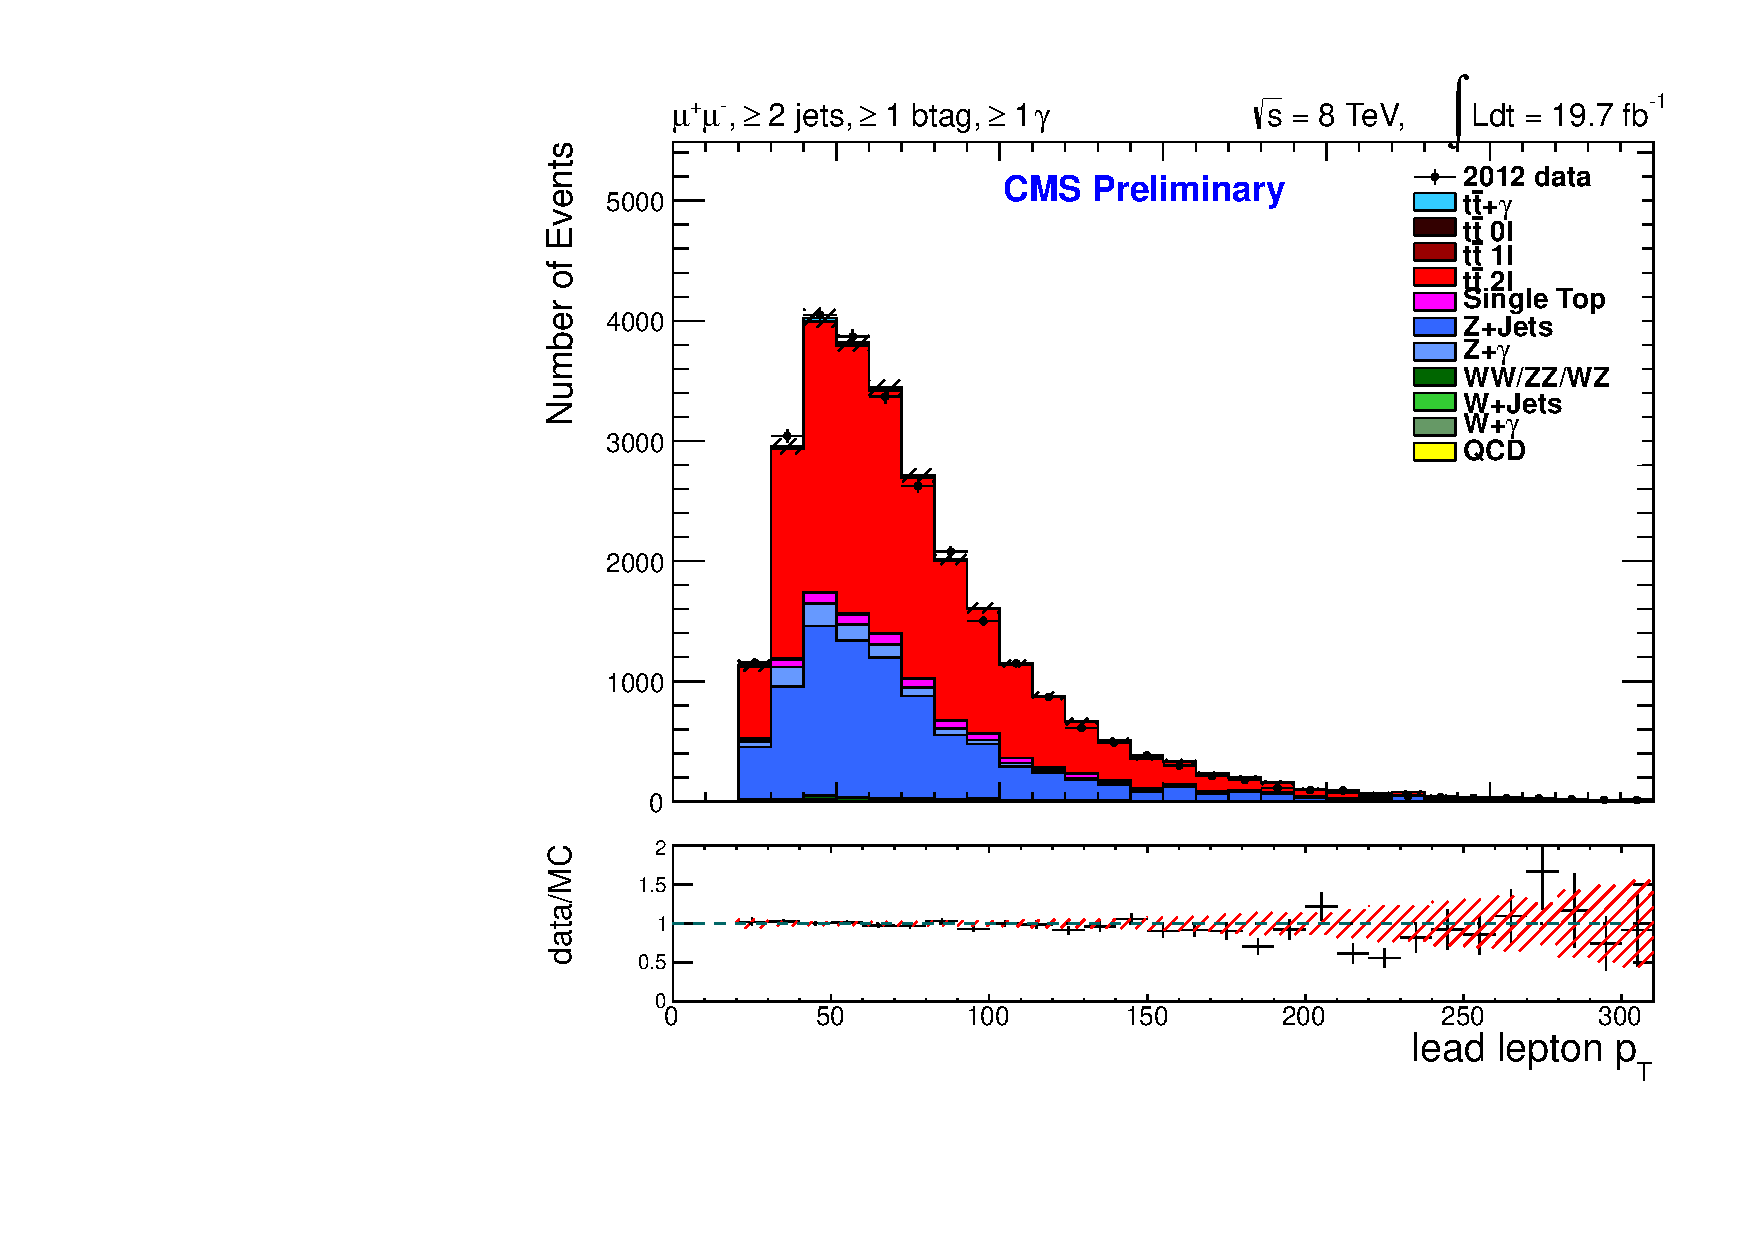
\includegraphics[width=0.5\textwidth]{Plots/ControlPlots/TTbarDiLeptonAnalysis/MuMu/DiLepton/LeadLepton_Pt_splitTTbar_ratio.pdf}
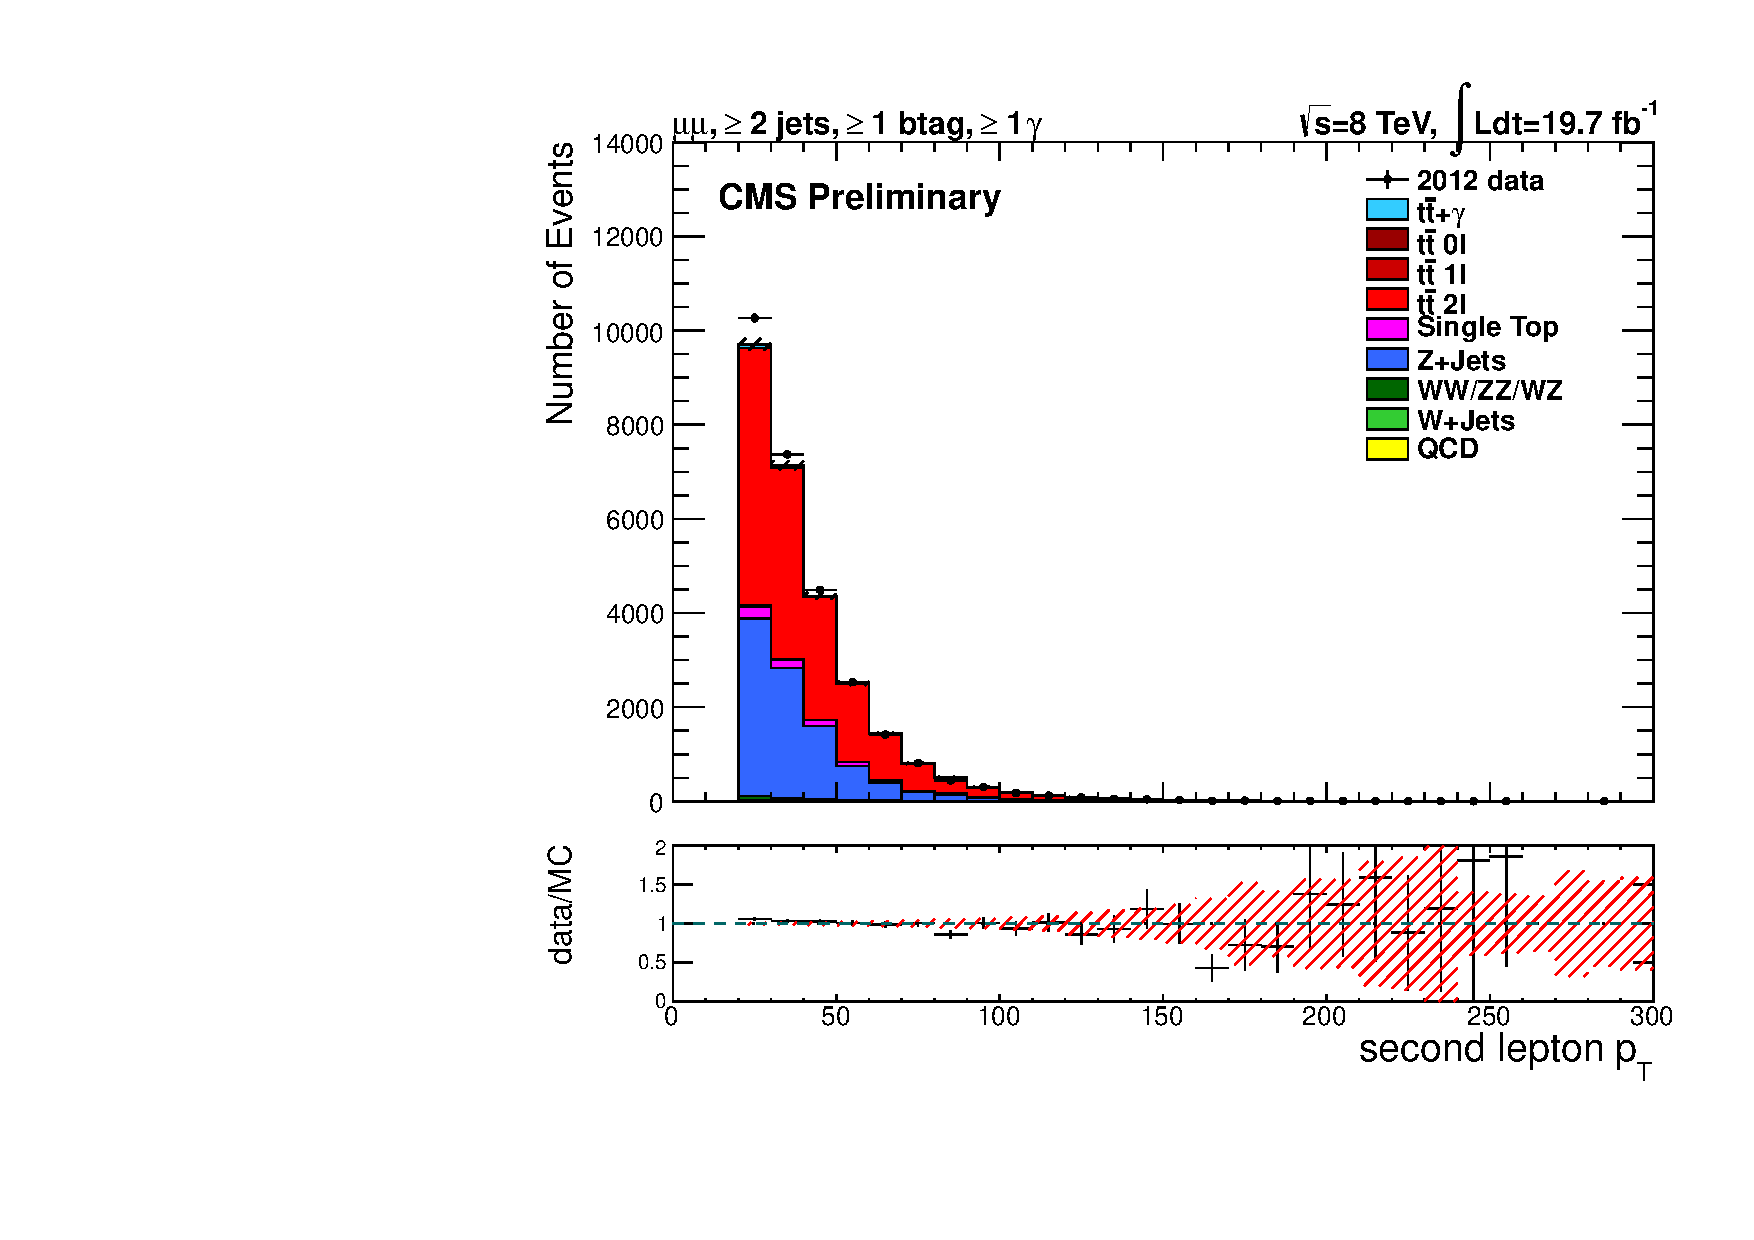
\includegraphics[width=0.5\textwidth]{Plots/ControlPlots/TTbarDiLeptonAnalysis/MuMu/DiLepton/SecondLepton_Pt_splitTTbar_ratio.pdf}\\
\begin{center}
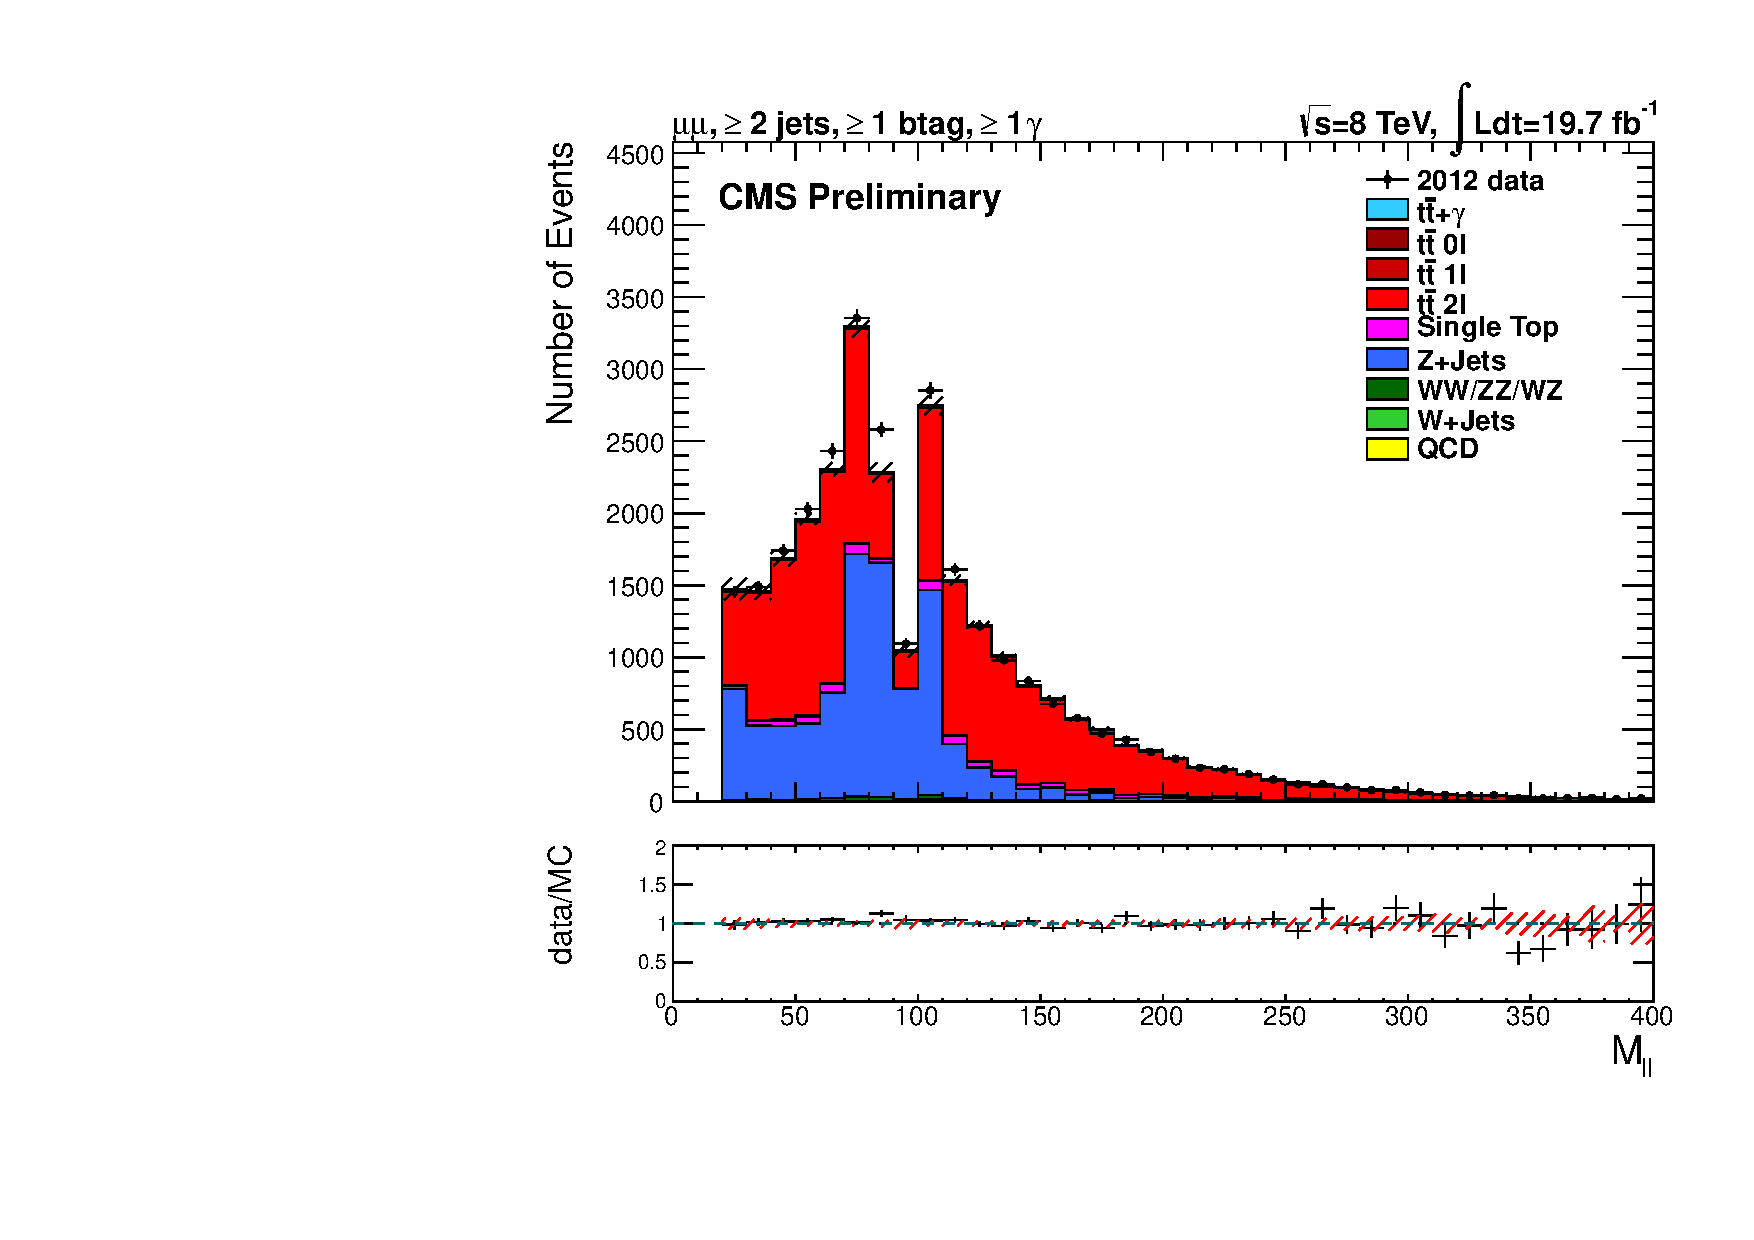
\includegraphics[width=0.5\textwidth]{Plots/ControlPlots/TTbarDiLeptonAnalysis/MuMu/DiLepton/diLepton_Mass_splitTTbar_ratio.pdf}
\end{center}
\caption{Lead lepton p$_T$ (top left), second lepton p$_T$ (top right), and dilepton mass (bottom) for the $\mu^{+}\mu^{-}$ channel only after $t\bar{t}$ selection.}
\label{fig-leptonPlots}
\end{figure}

\section{Jet Selection and b-tag Requirements} \label{sec-JetSelection}

Jets are reconstructed with the PF AK5 algorithm, anti-$k_T$ with jet size parameter (R) of 5 in the jet reconstruction model, and the following selections are made (PF loose Jet ID). Before applying any selection the following corrections are made to account for imperfect jet energy measurement: Jet Energy Scale correction, and Jet Energy Resolution smearing, as described in Section \ref{subsec-JetReconstruction}. After jets are identified and reconstructed, the following set of cuts are implemented with the requirements:

\begin{itemize}
	\item Transverse momentum greater than 30 GeV
	\item Absolute value of pseudorapidity less than 2.4
	\item Number of constituents greater than 1
	\item Charge multiplicity greater than 0
	\item Neutral hadron fraction of energy less than 0.99
	\item Neutral electromagnetic energy fraction less than 0.99
	\item Charged EM energy fraction less than 0.99
	\item Charged hadron energy fraction greater than 0
\end{itemize}

These cuts help to avoid picking detector noise and ECAL spikes as jets. We also impose a selection criterion that if a lepton lies within a cone of $\Delta R = 0.3$, then the lepton is included within the jet calculation. CMS improves the quality of reconstructed jets by the requirement that the energy deposits from a jet are recorded in both the ECAL and HCAL, where jets that manifest from anomalous deposits of energy in just one of the sub-detector are able to be removed from the sample \cite{CMS-PAS-JME-10-003}.

 \textbf{B-tagged jets} are identified with the Combined Secondary Vertex b-tagging algorithm using the loose working point (CSVL). Event re-weighting is applied to correct for the difference in b-tagging efficiency in data and simulation as explained in Section \ref{subsec-SimulatedEventsCorrection}. The loose working point refers to a b-tagging efficiency of  and a misidentification probability of 24.4\%.

 In each channel the requirement of at least 2 good jets, where a good jet passes all the aforementioned selection requirements, and at least one b-jet. By applying these requirements the contribution from the most prominent backgrounds, $t\bar{t}$ and events with additional loose jets, are removed. 

\begin{figure}
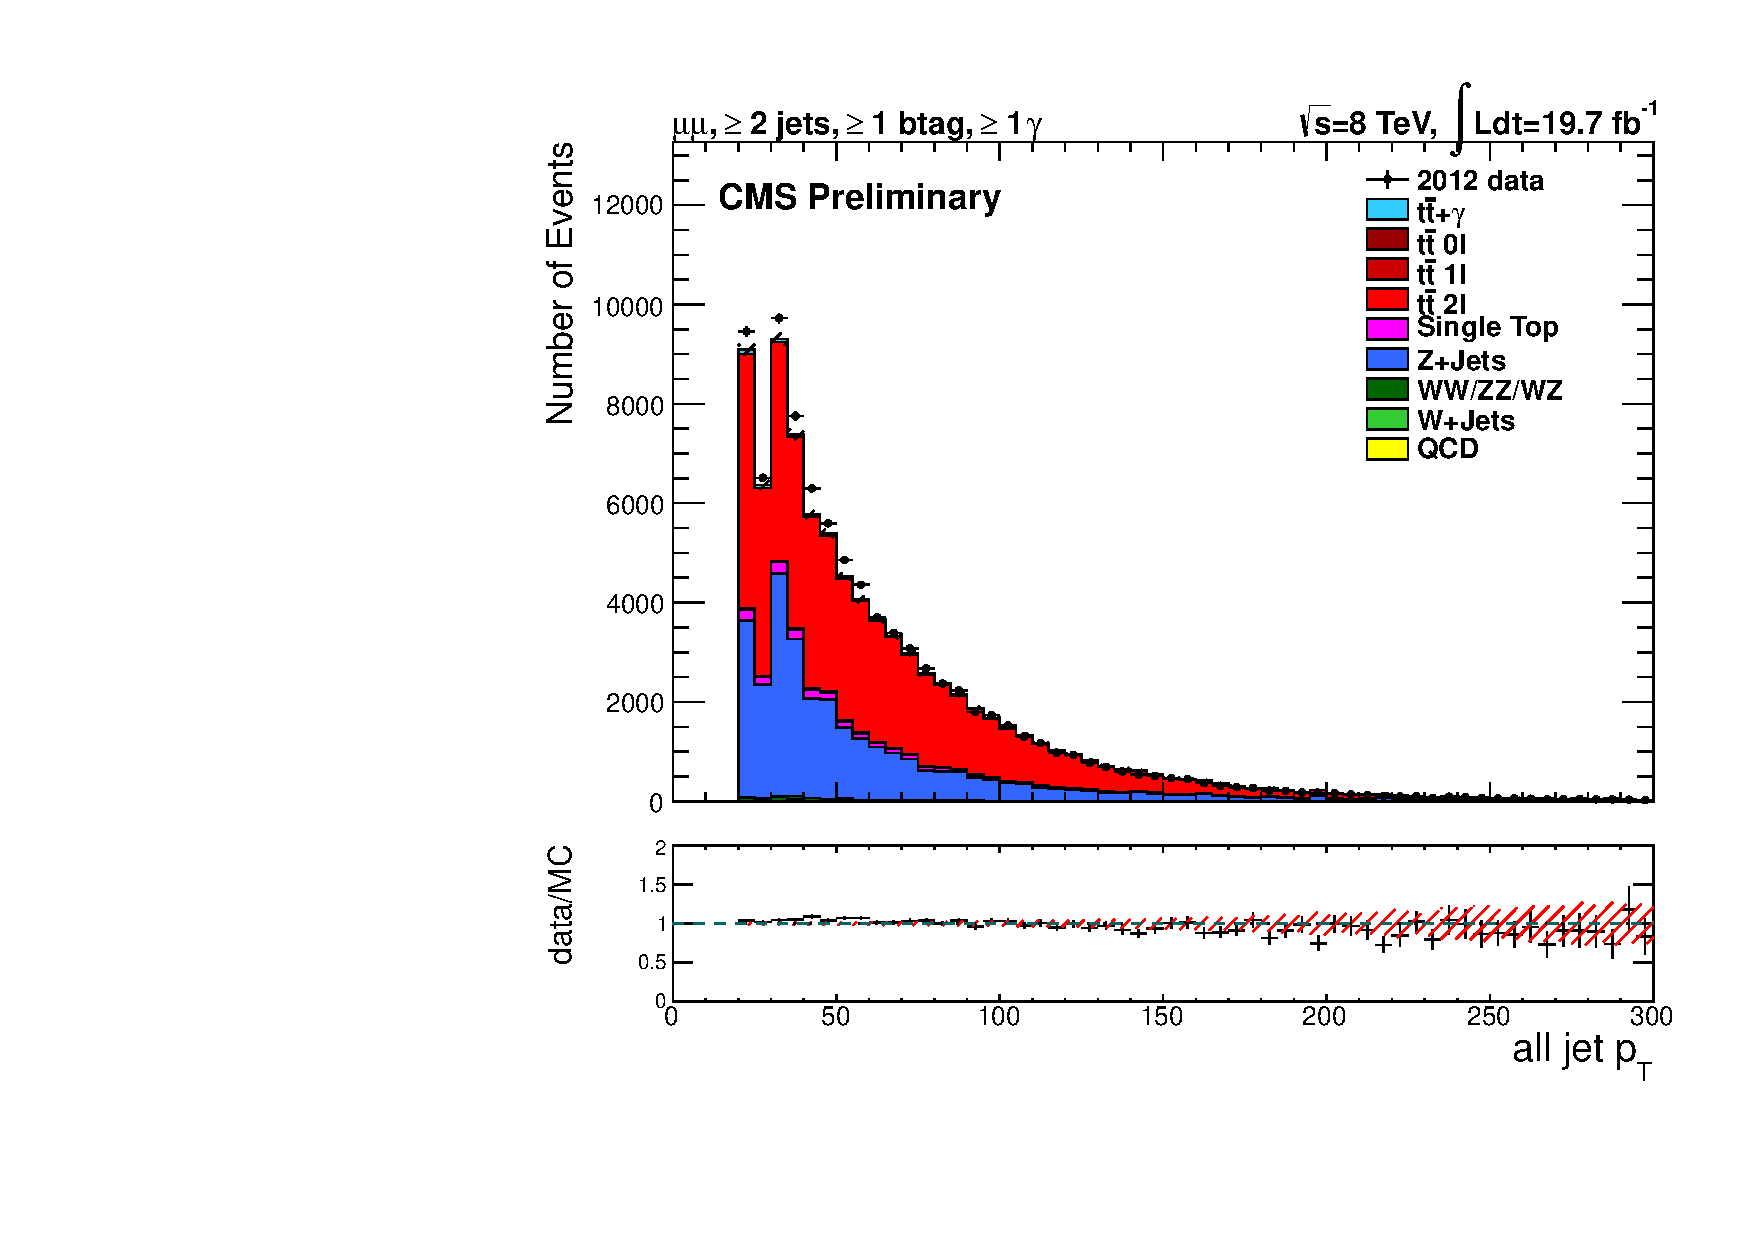
\includegraphics[width=0.5\textwidth]{Plots/ControlPlots/TTbarDiLeptonAnalysis/MuMu/Jets/all_jet_pT_splitTTbar_ratio.pdf}
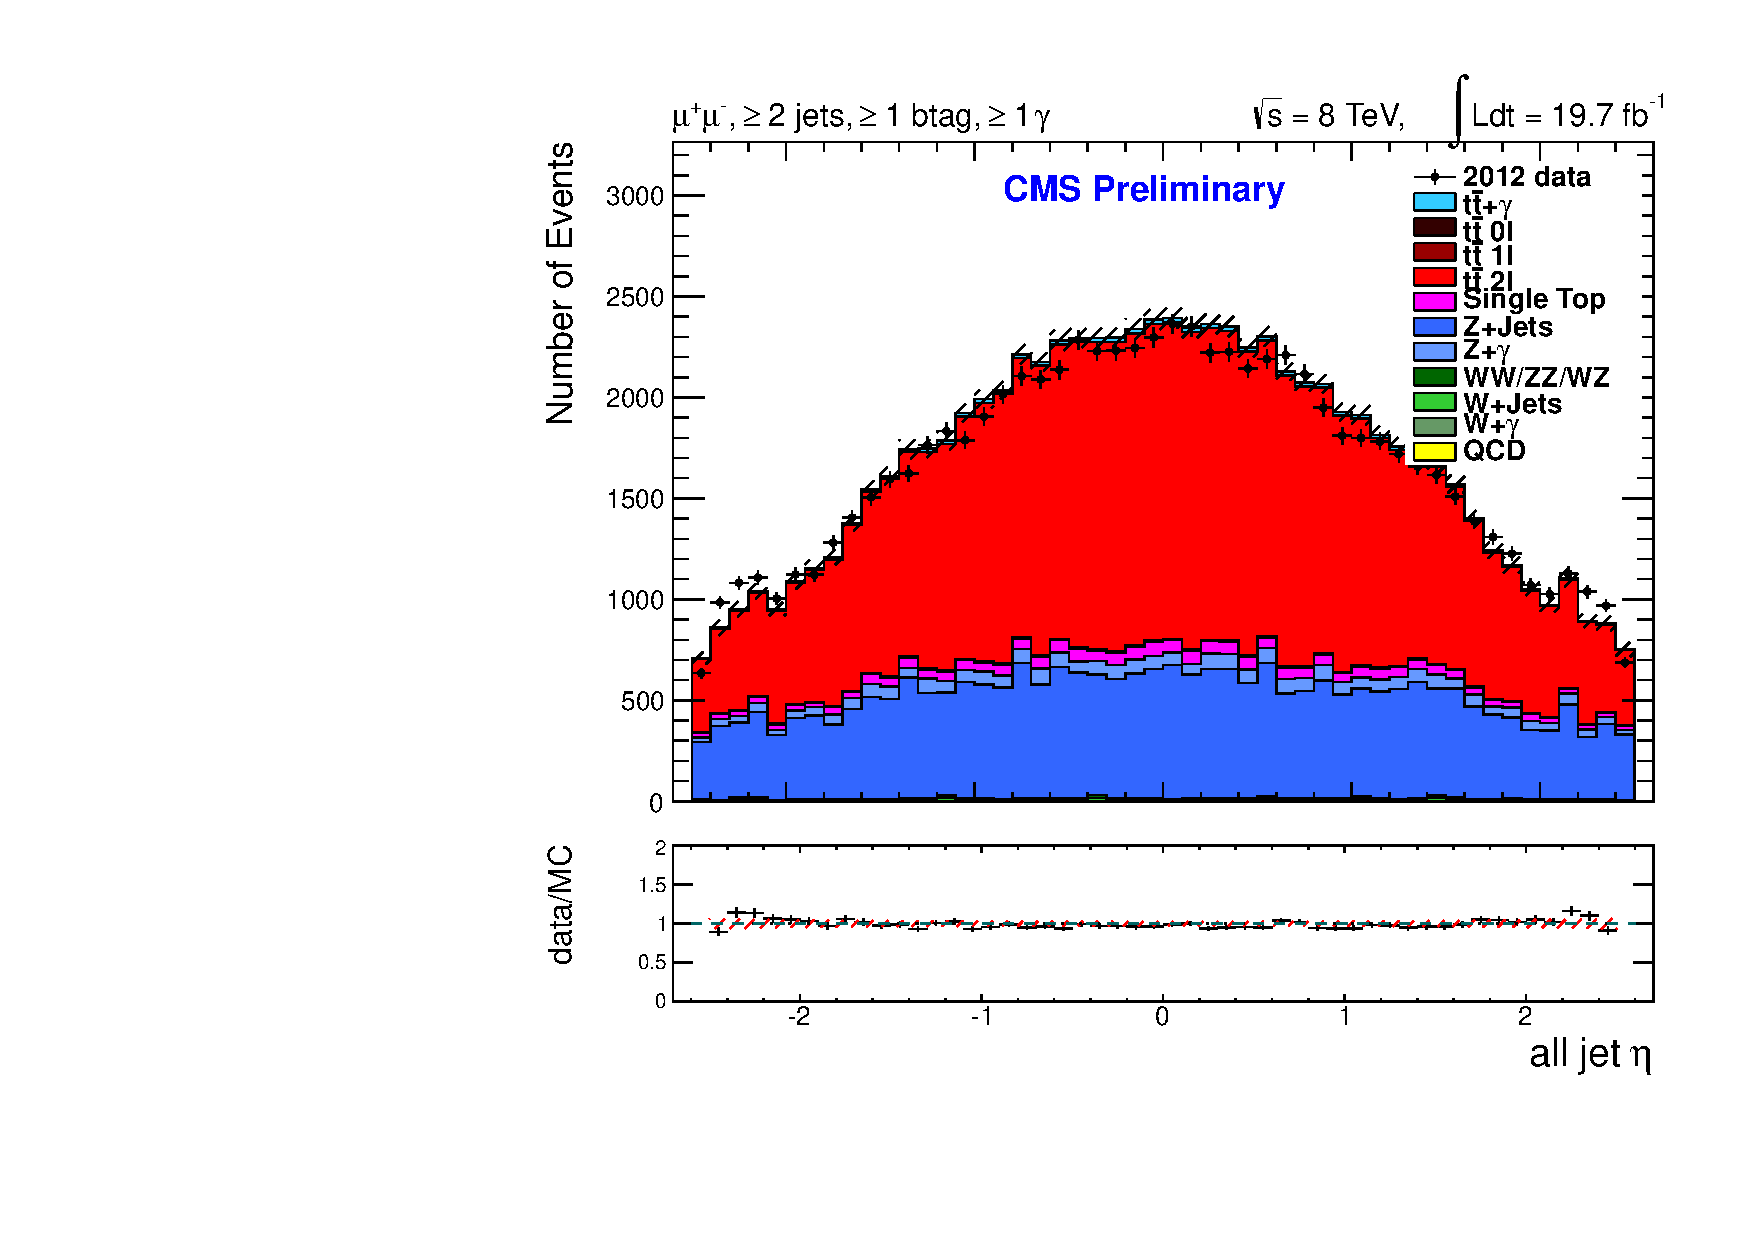
\includegraphics[width=0.5\textwidth]{Plots/ControlPlots/TTbarDiLeptonAnalysis/MuMu/Jets/all_jet_eta_splitTTbar_ratio.pdf}\\
\begin{center}
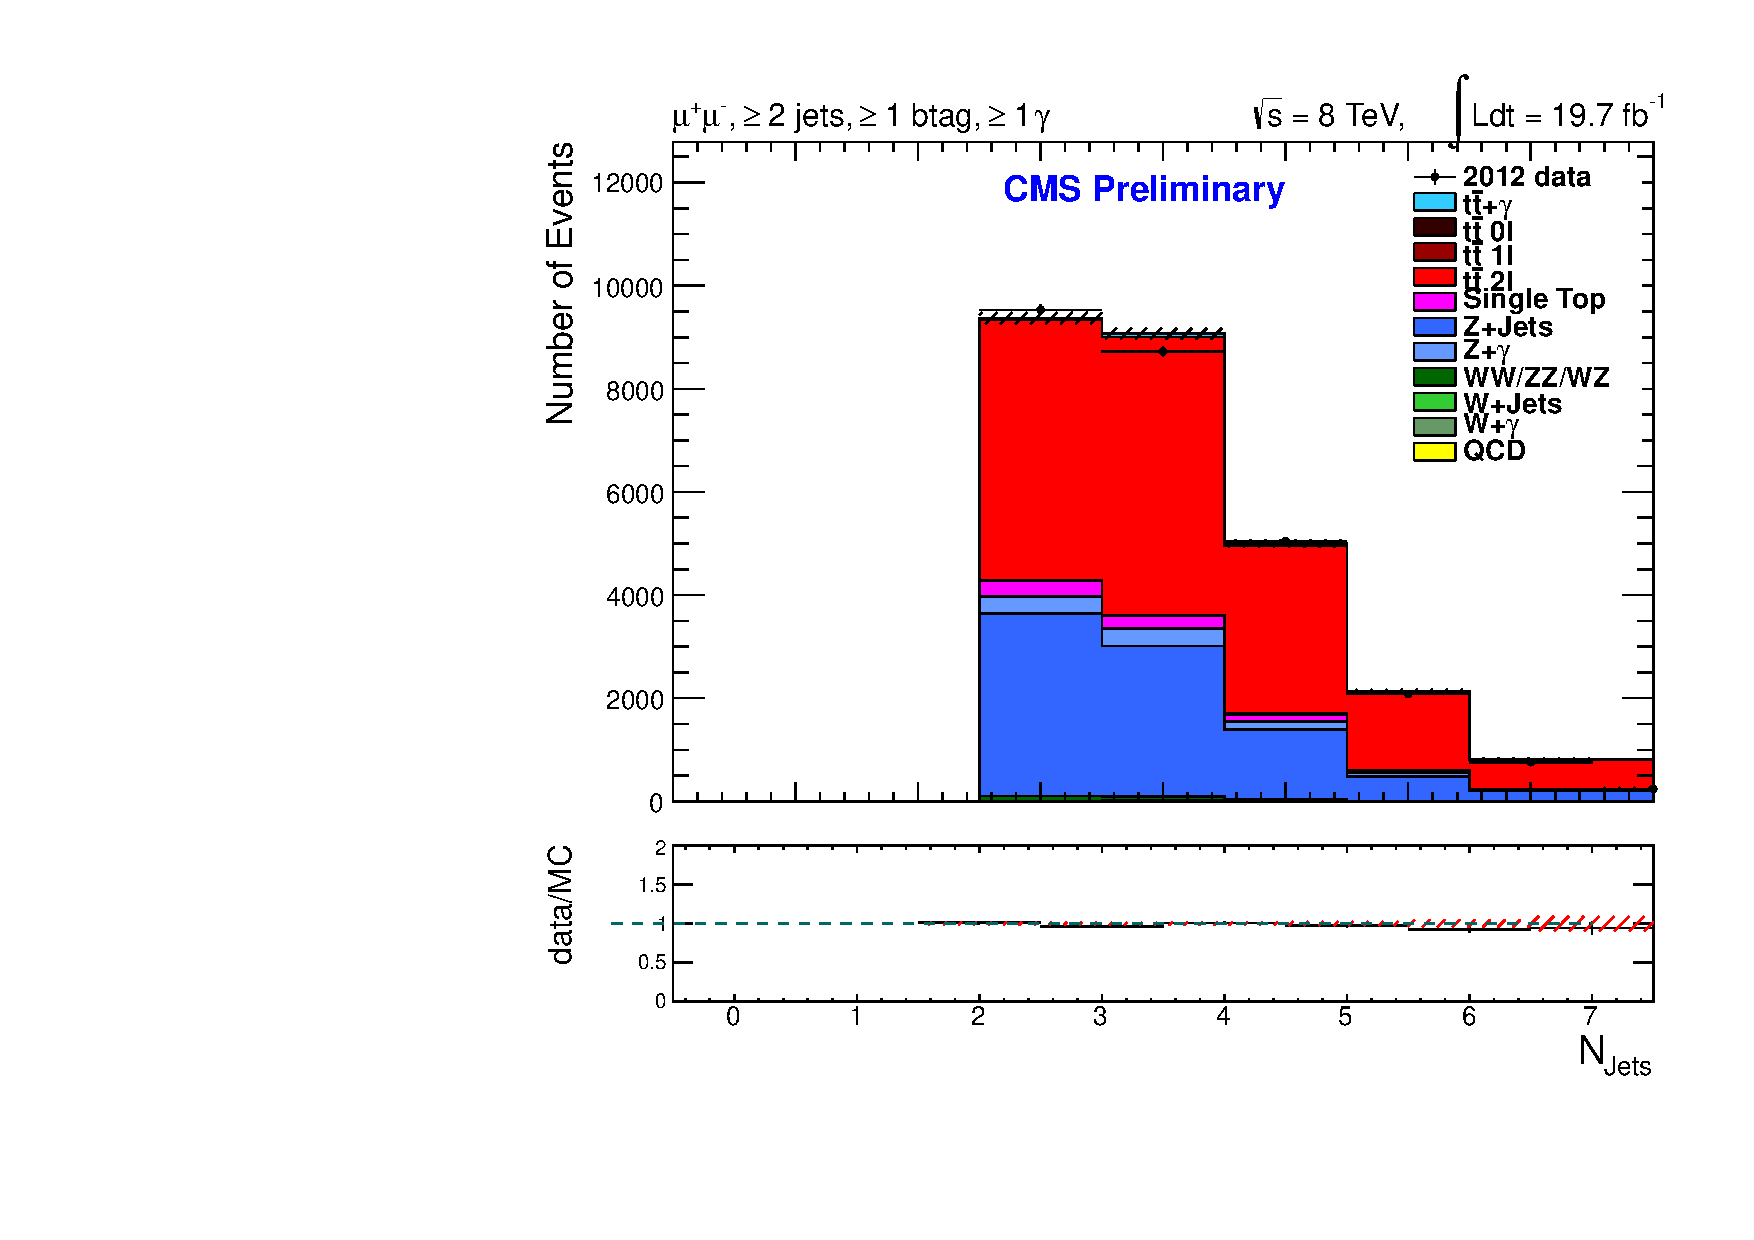
\includegraphics[width=0.5\textwidth]{Plots/ControlPlots/TTbarDiLeptonAnalysis/MuMu/Jets/N_Jets_splitTTbar_ratio.pdf}
\end{center}
\caption{Comparison of the sum of the transverse momentum and $\eta$ in all reconstructed jets (top), and number of jets (bottom) per event for the $\mu^{+}\mu^{-}$ channel only after $t\bar{t}$ selection.}
\label{fig-jetPlots}
\end{figure}
 
\section{Missing Transverse Energy} \label{sec-METSelection}

The missing transverse energy (MET) selection cut is implemented only within the di-muon and di-electron channels as the mixed channel is better defined with different flavour quarks in the final state, and therefore less likely to be misreconstructed in the detector. Due to the small cross-section of the $t\bar{t}+\gamma$ decay, and the much smaller branching ratio of the dilepton channel relative to the semileptonic channel, a MET cut of $>20$ GeV is used in order to increase statistics. Figure \ref{fig-METplots} shows the MET, the azimuthal angle $\phi$ of the MET, and the MET significance, where the MET significance assesses on an event-by-event basis the likelihood that an observed MET is consistent with a fluctuation from zero due to detector-related limitations, such as finite measurement resolution. 

\begin{figure}
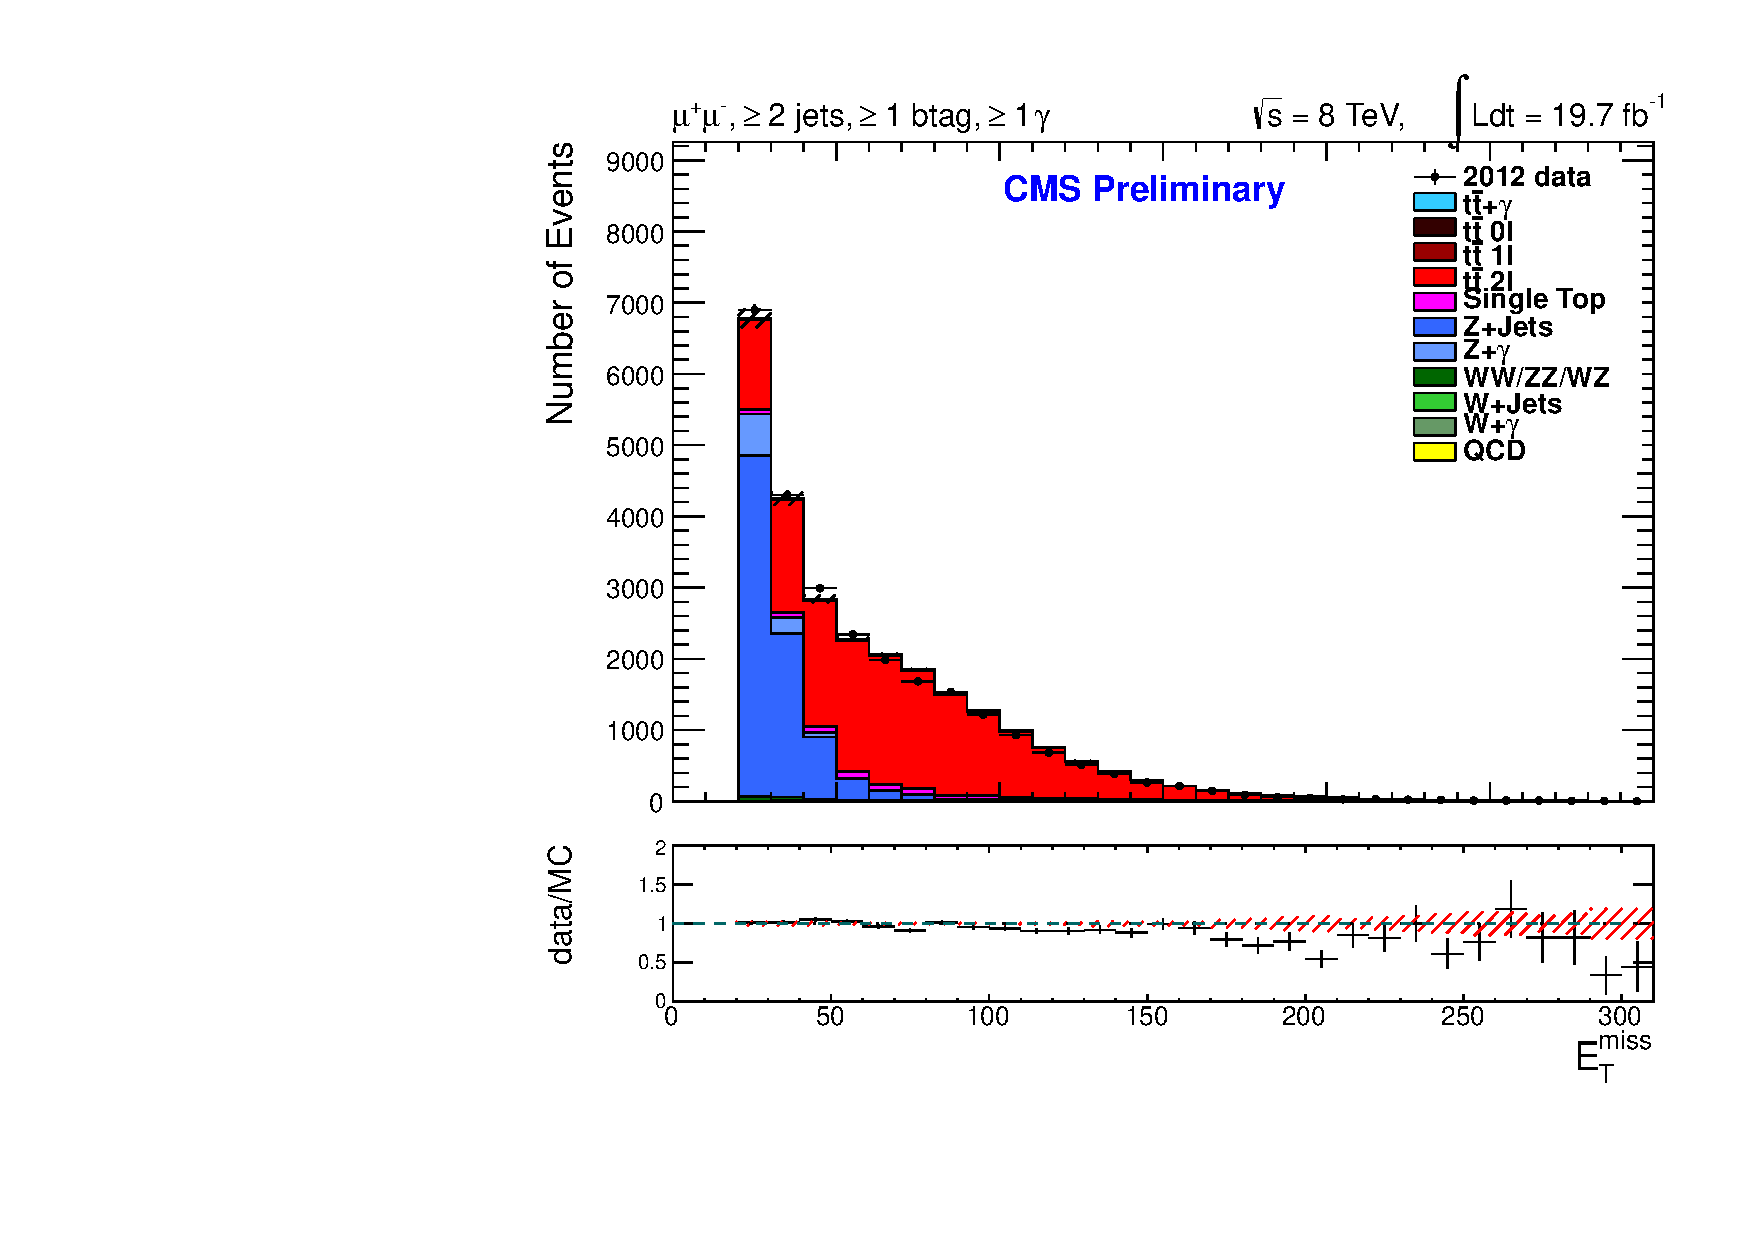
\includegraphics[width=0.5\textwidth]{Plots/ControlPlots/TTbarDiLeptonAnalysis/MuMu/MET/patType1CorrectedPFMet/MET_splitTTbar_ratio.pdf}
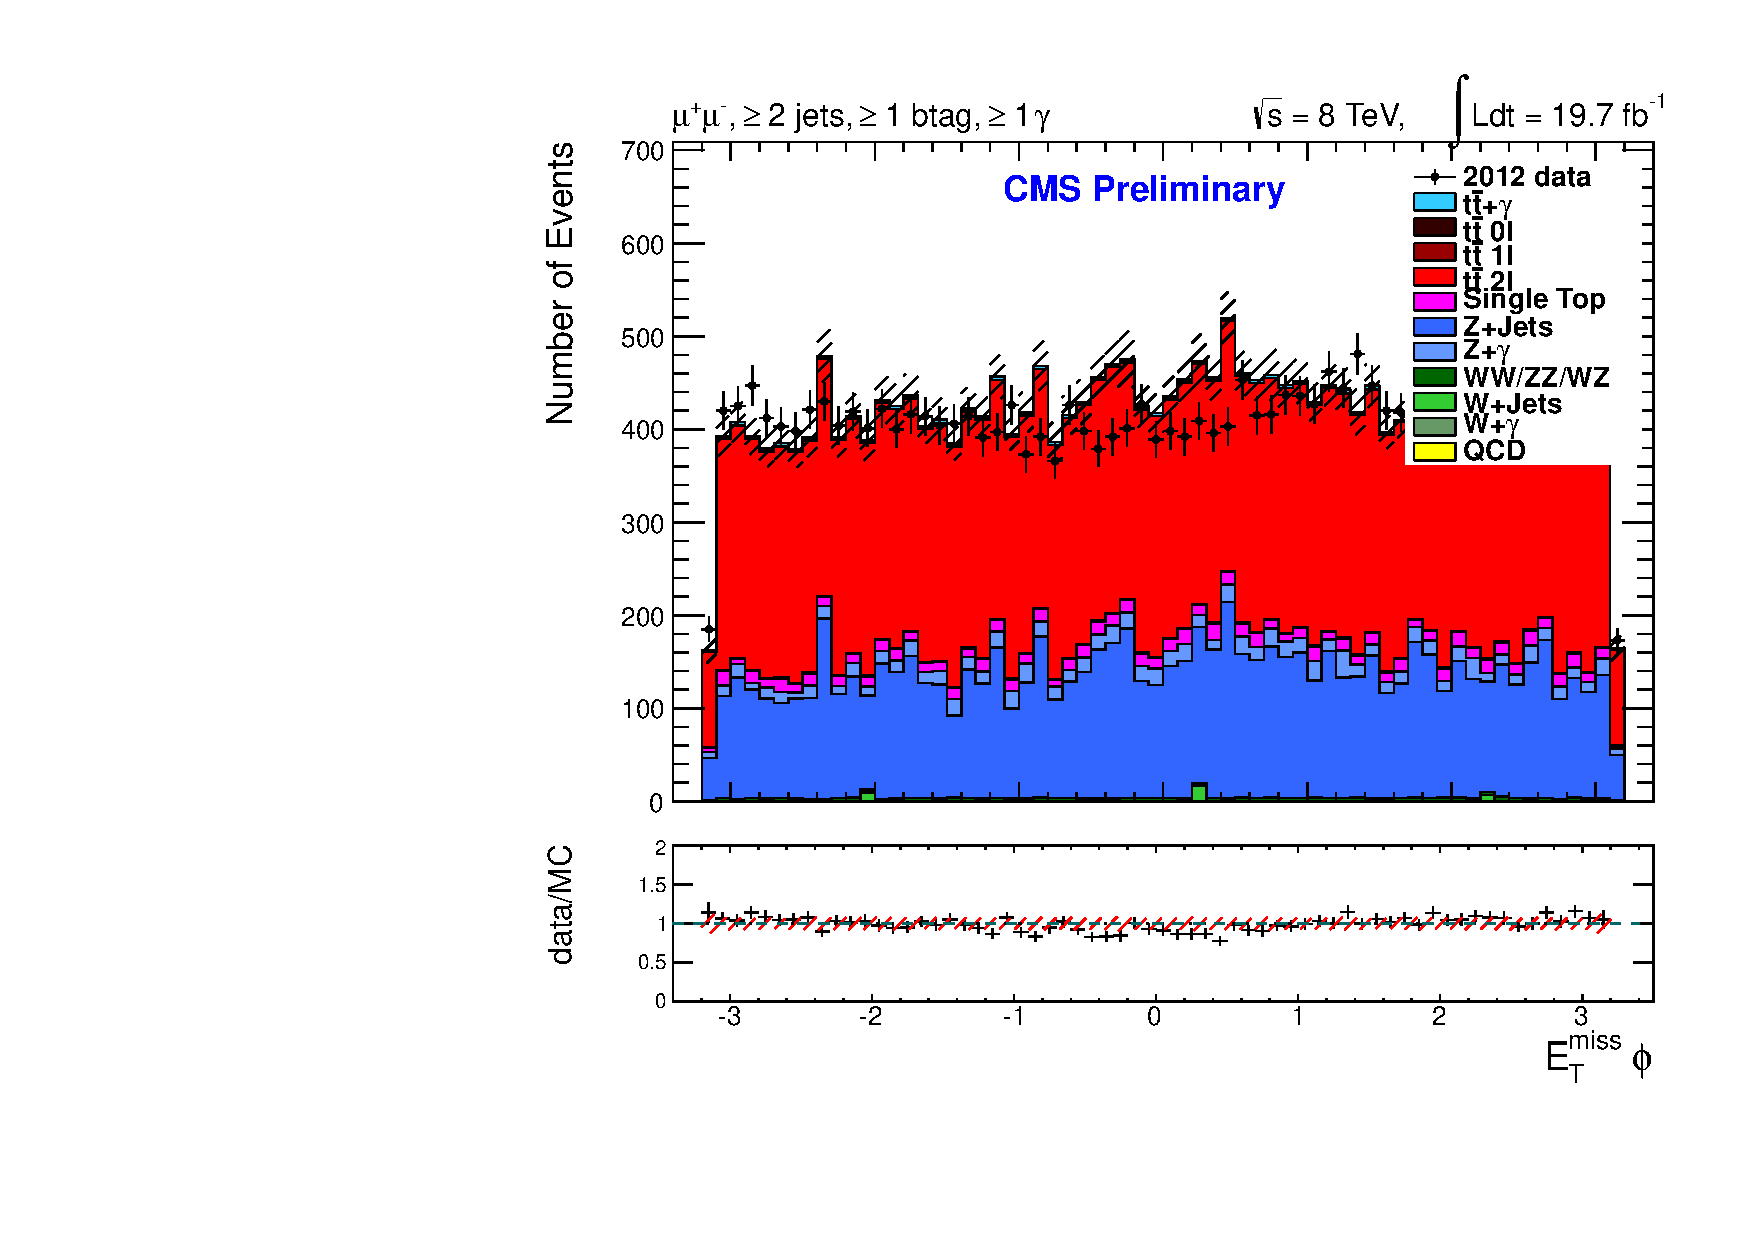
\includegraphics[width=0.5\textwidth]{Plots/ControlPlots/TTbarDiLeptonAnalysis/MuMu/MET/patType1CorrectedPFMet/MET_phi_splitTTbar_ratio.pdf}\\
\begin{center}
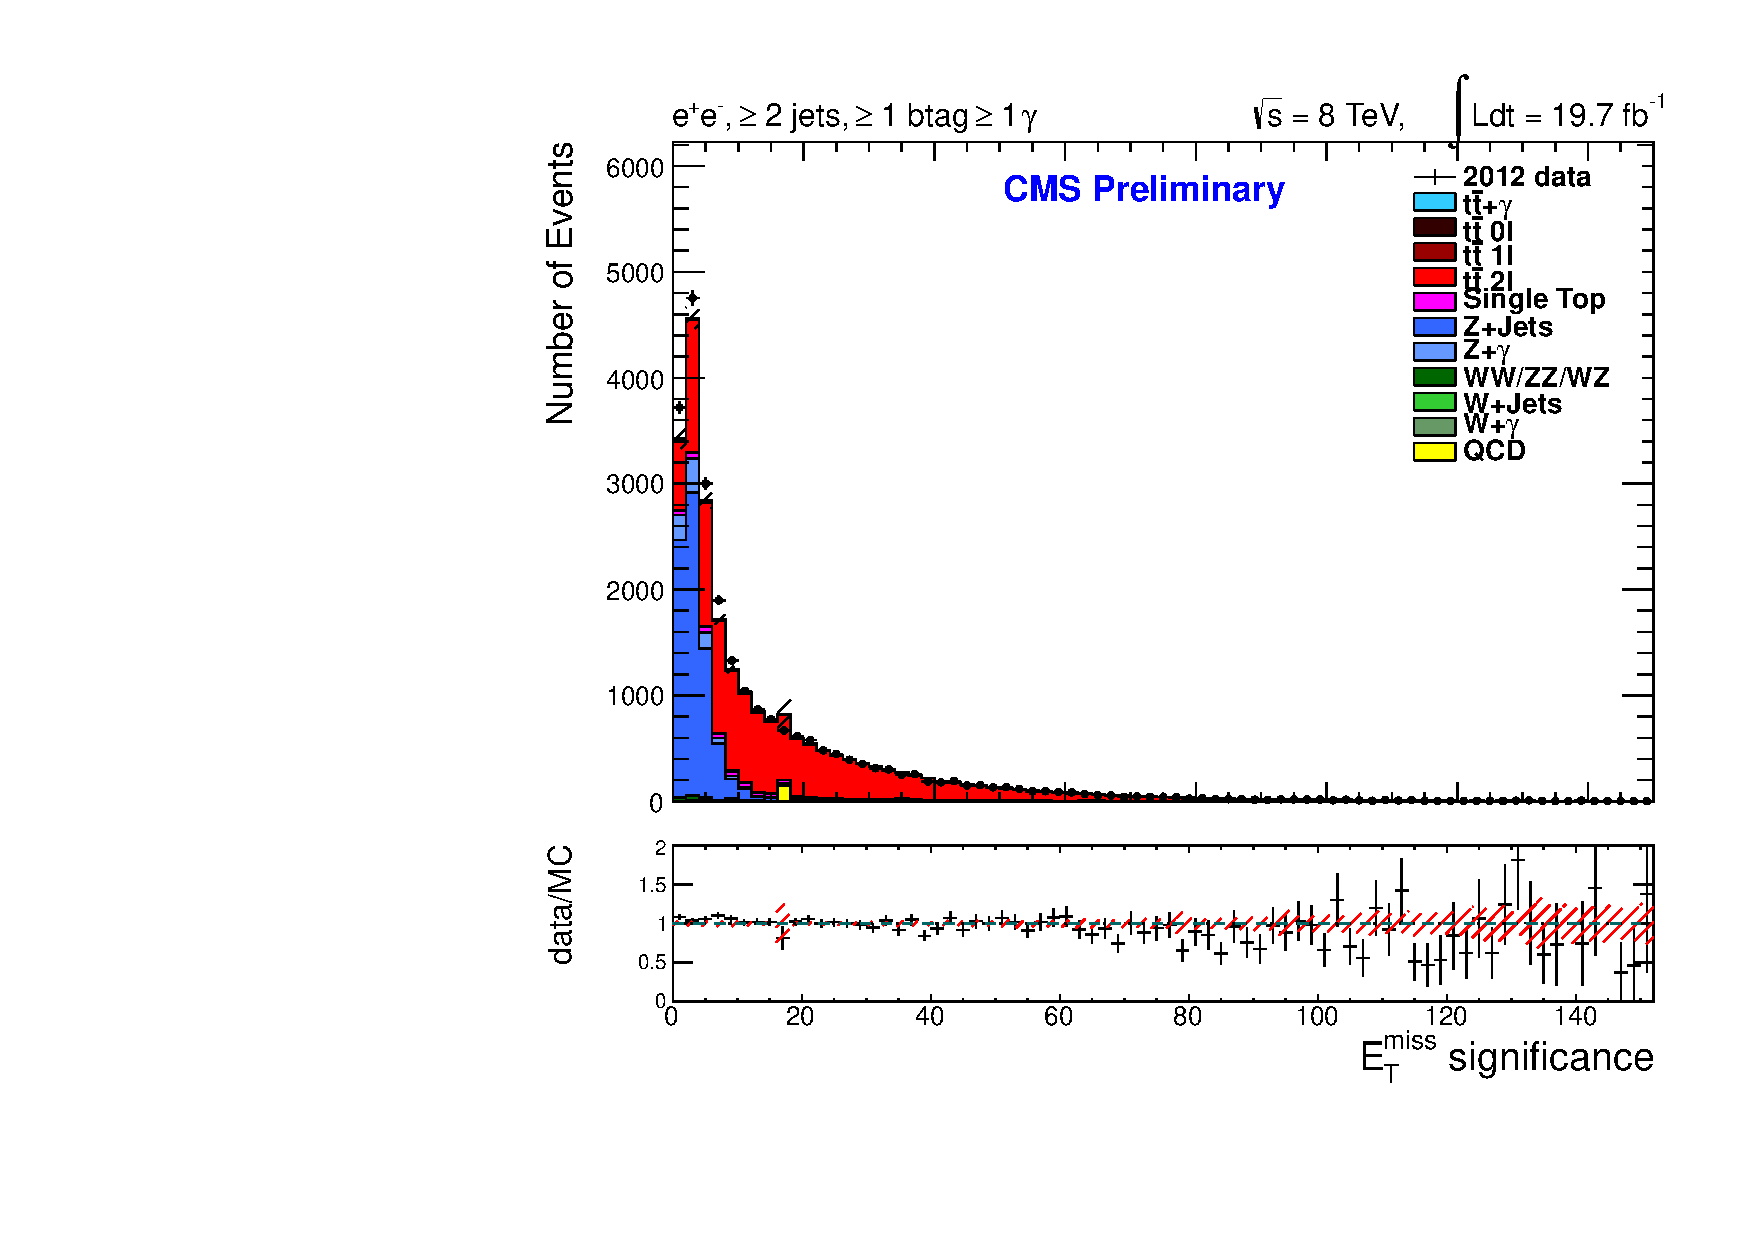
\includegraphics[width=0.5\textwidth]{Plots/ControlPlots/TTbarDiLeptonAnalysis/EE/MET/patType1CorrectedPFMet/METsignificance_splitTTbar_ratio.pdf}
\end{center}
\caption{The missing transverse energy distributions in terms of missing energy, azimuthal angle $\phi$, and MET significance for the $\mu^{+}\mu^{-}$ channel only after $t\bar{t}$ selection.}
\label{fig-METplots}
\end{figure}

\subsection{Corrections to simulated events} \label{subsec-SimulatedEventsCorrection}


\begin{figure}
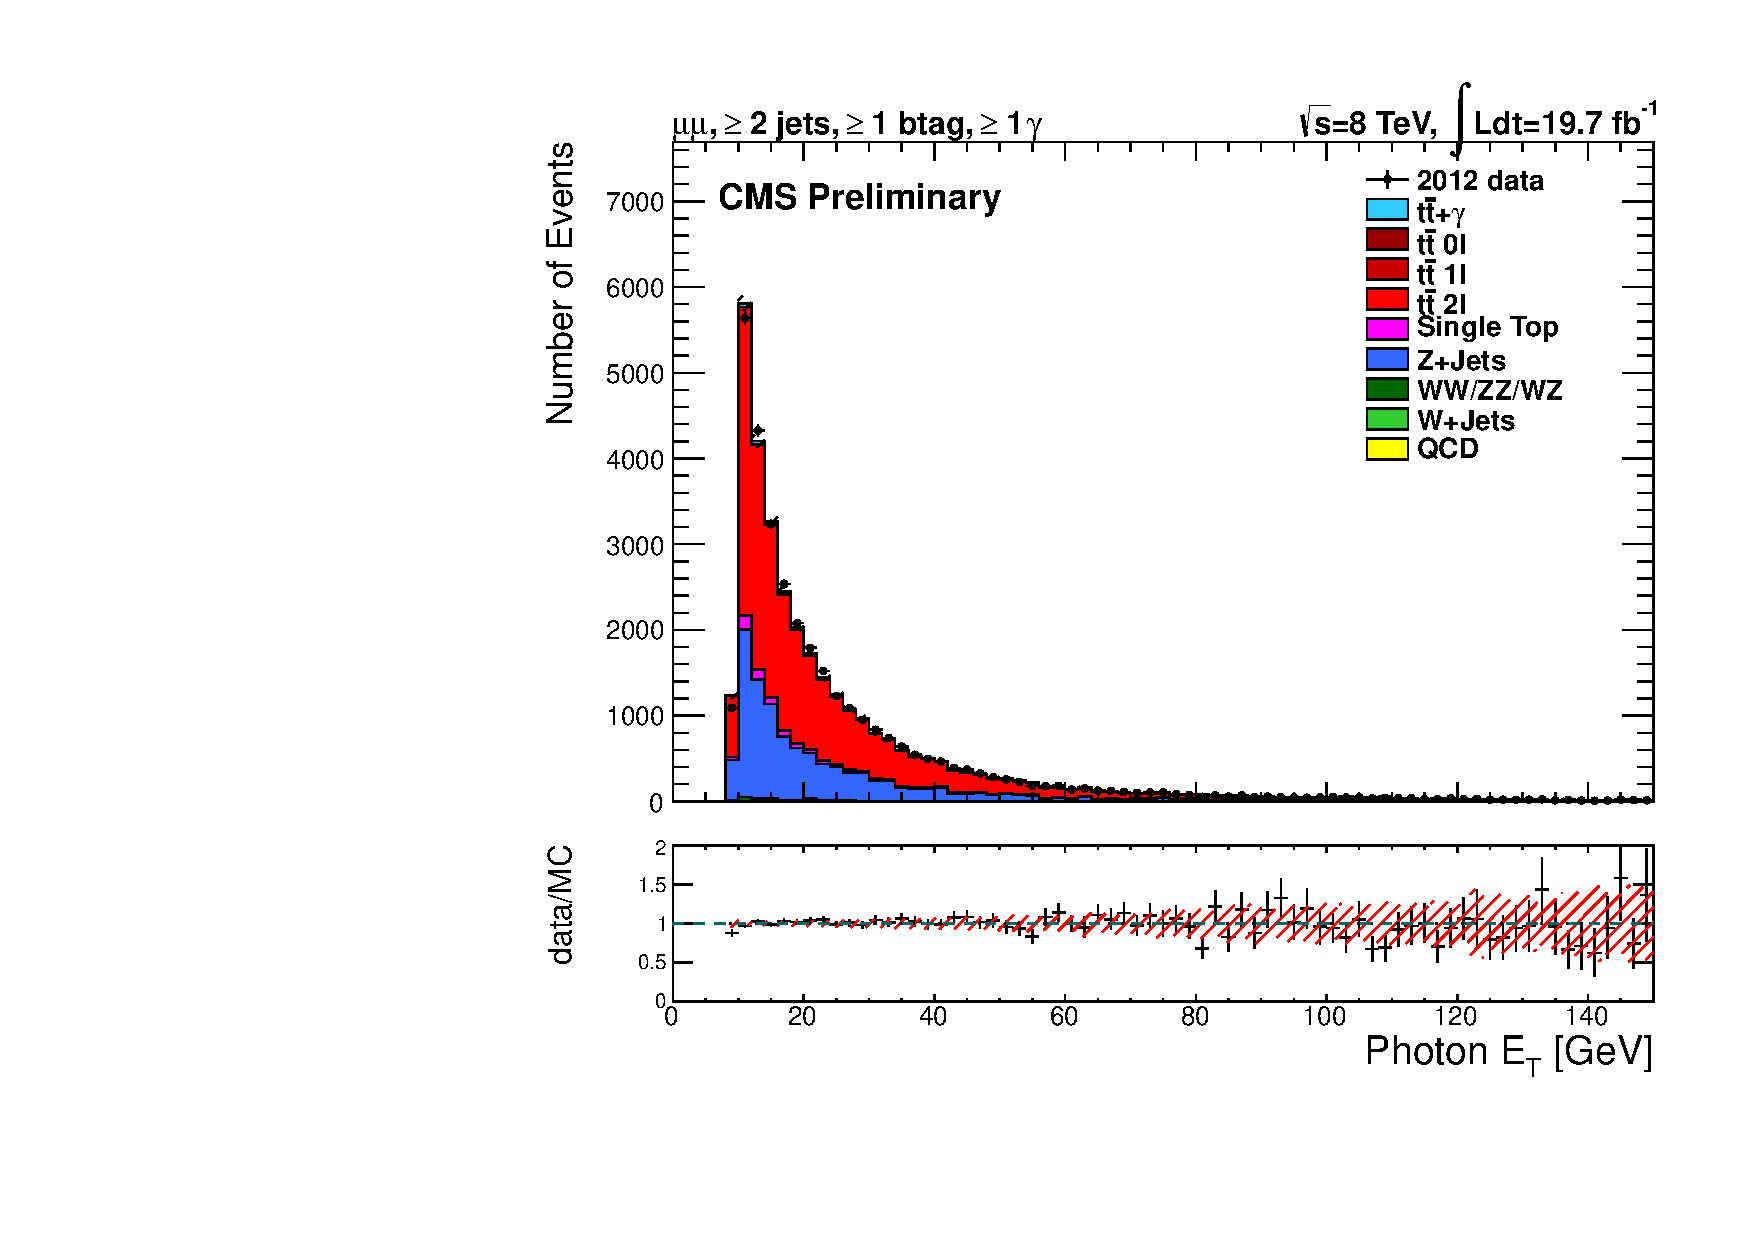
\includegraphics[width=0.5\textwidth]{Plots/ControlPlots/TTbarDiLeptonAnalysis/MuMu/Photons/AllPhotons/Photon_ET_splitTTbar_ratio.pdf}
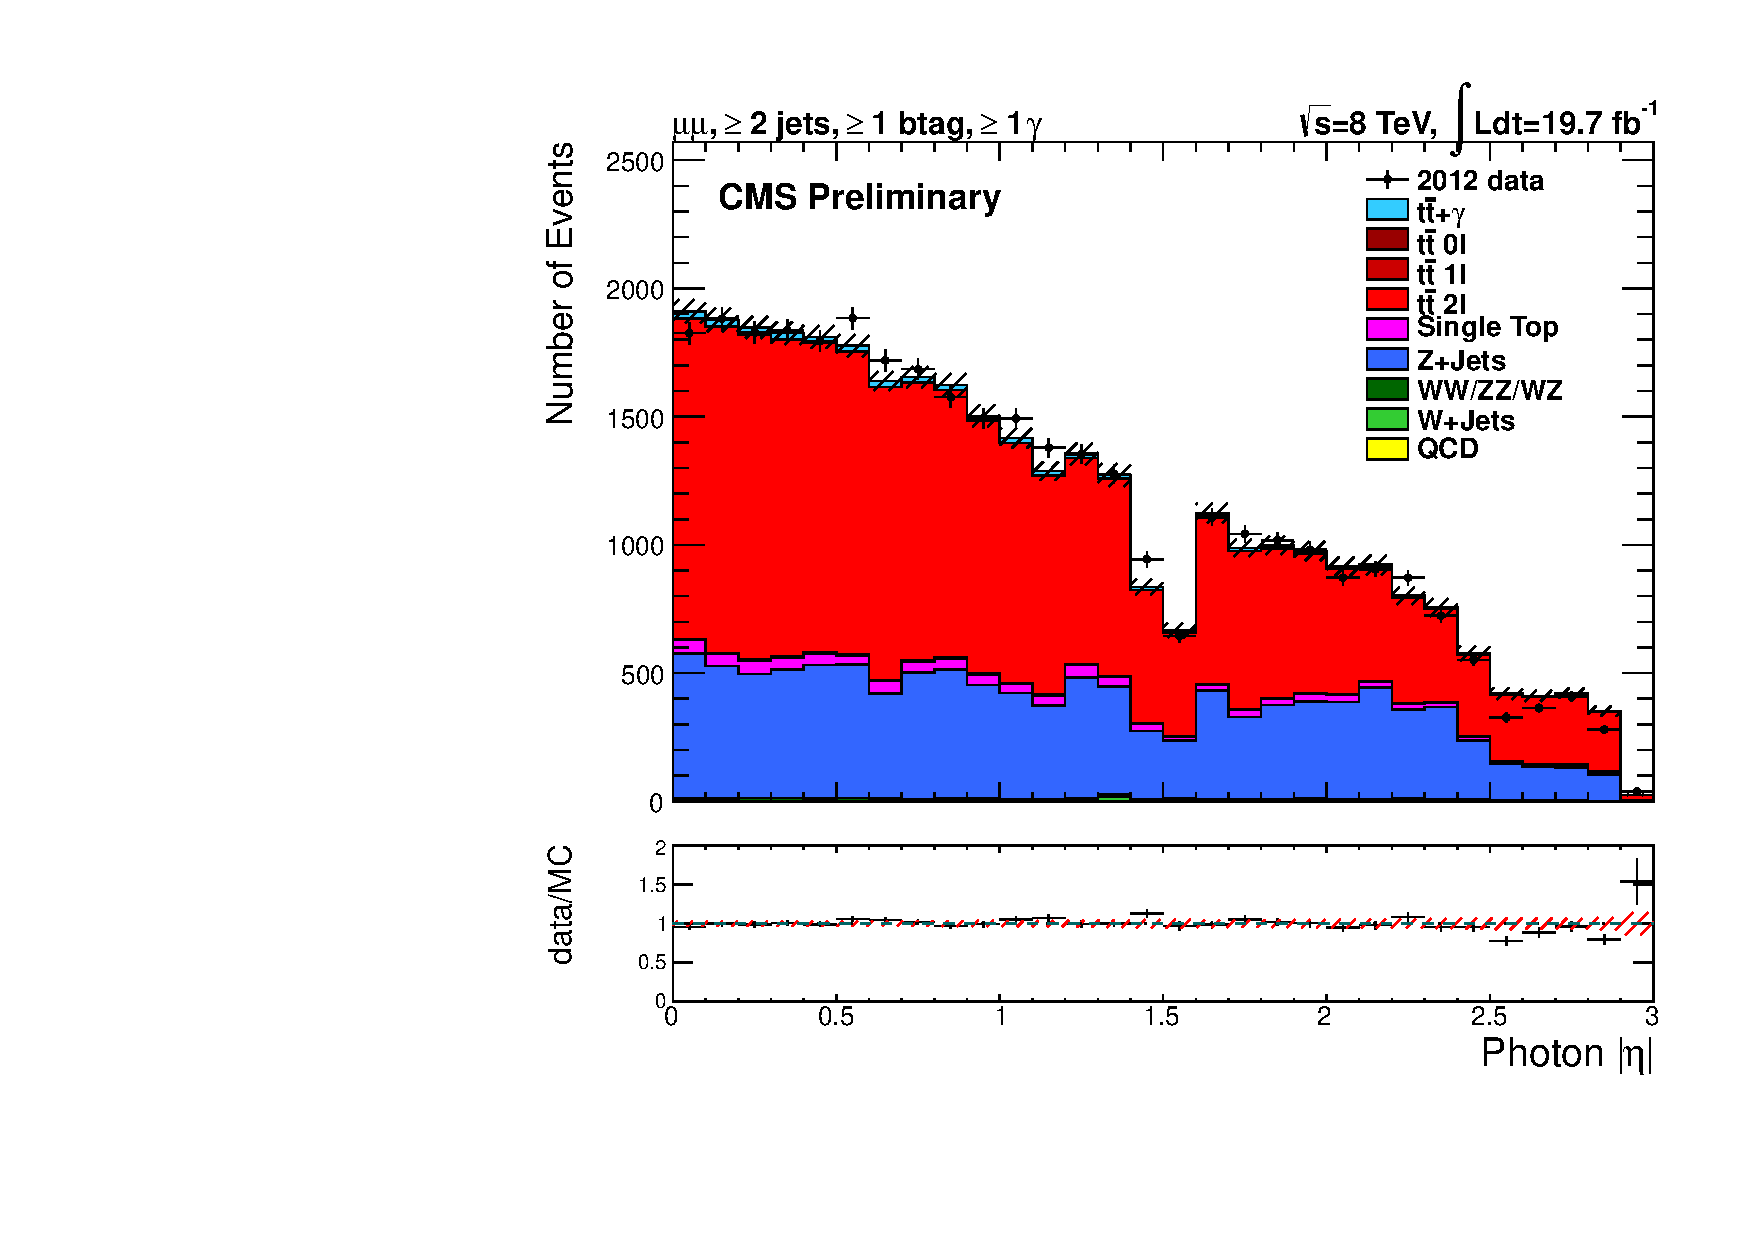
\includegraphics[width=0.5\textwidth]{Plots/ControlPlots/TTbarDiLeptonAnalysis/MuMu/Photons/AllPhotons/Photon_AbsEta_splitTTbar_ratio.pdf}\\
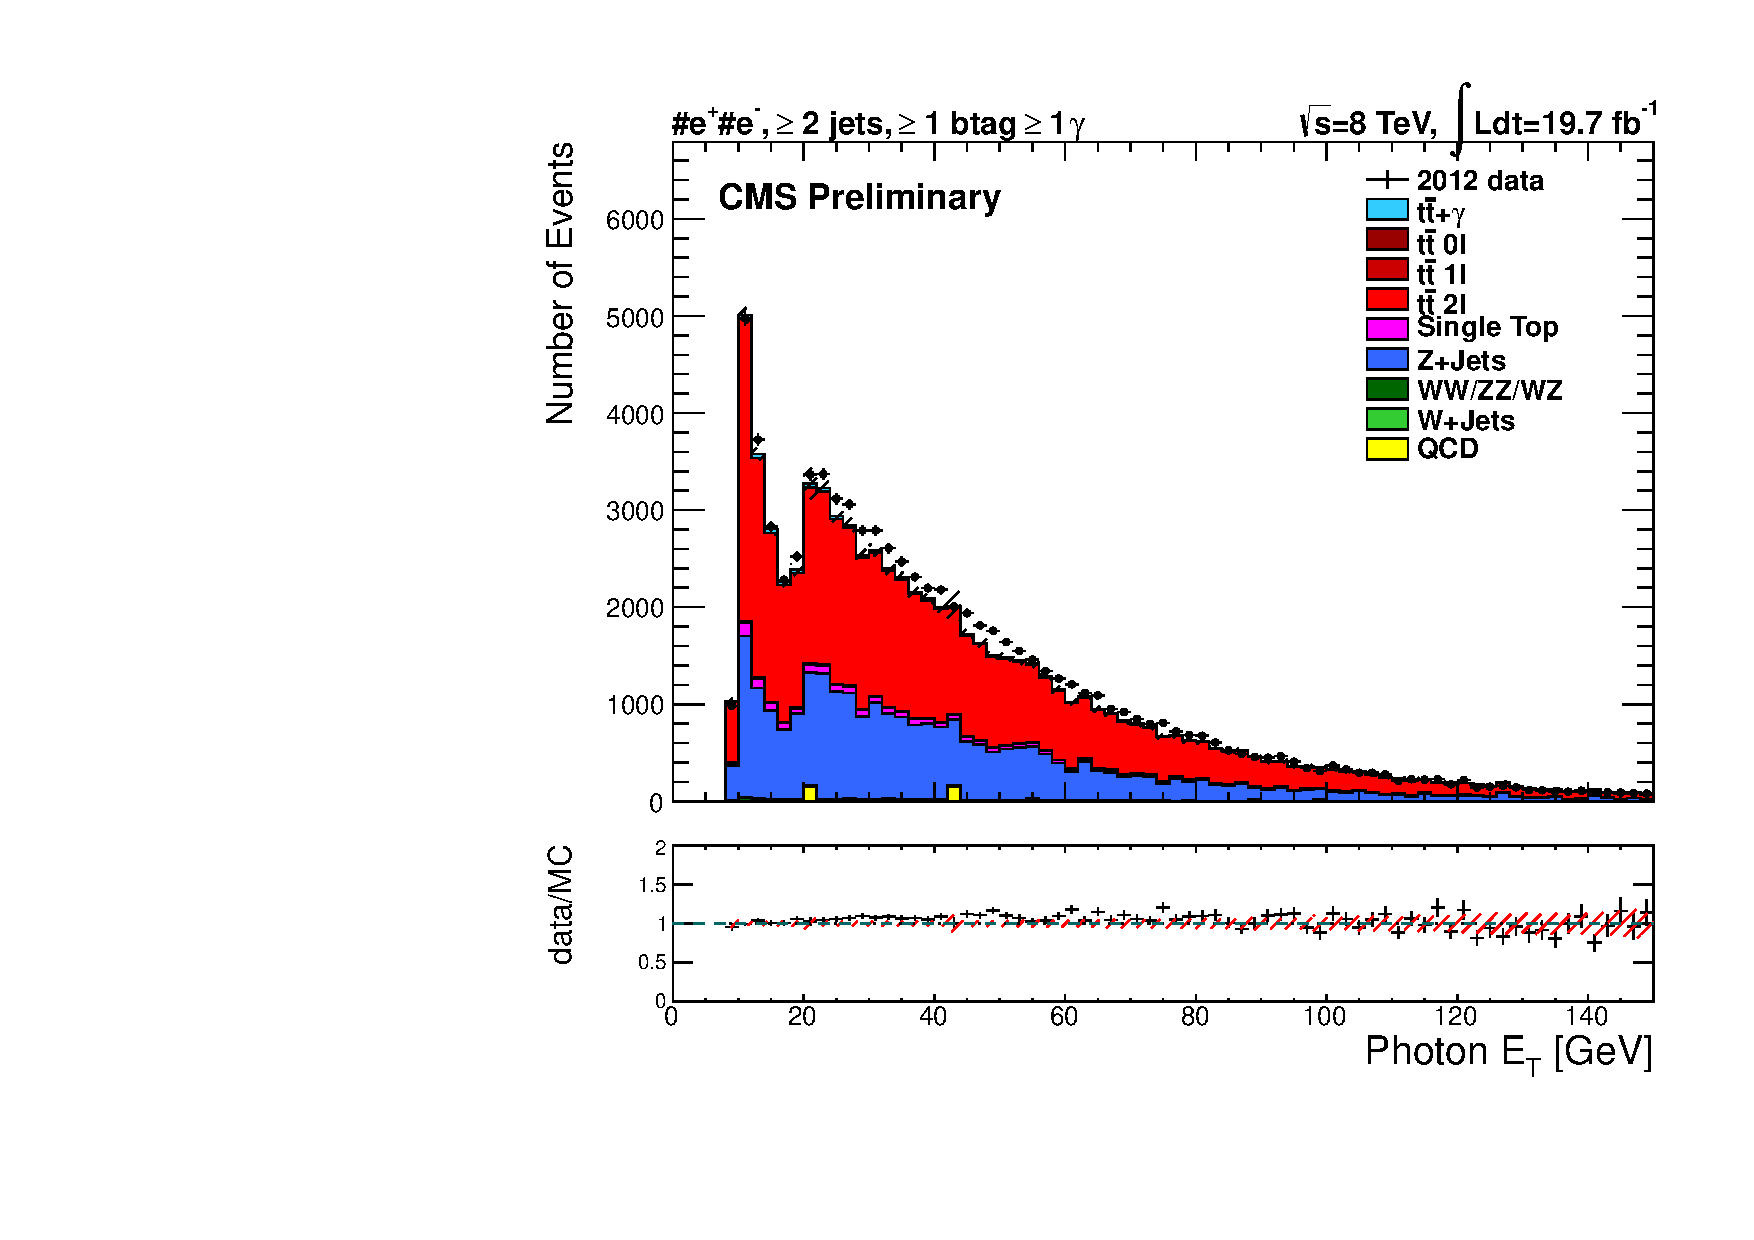
\includegraphics[width=0.5\textwidth]{Plots/ControlPlots/TTbarDiLeptonAnalysis/EE/Photons/AllPhotons/Photon_ET_splitTTbar_ratio.pdf}
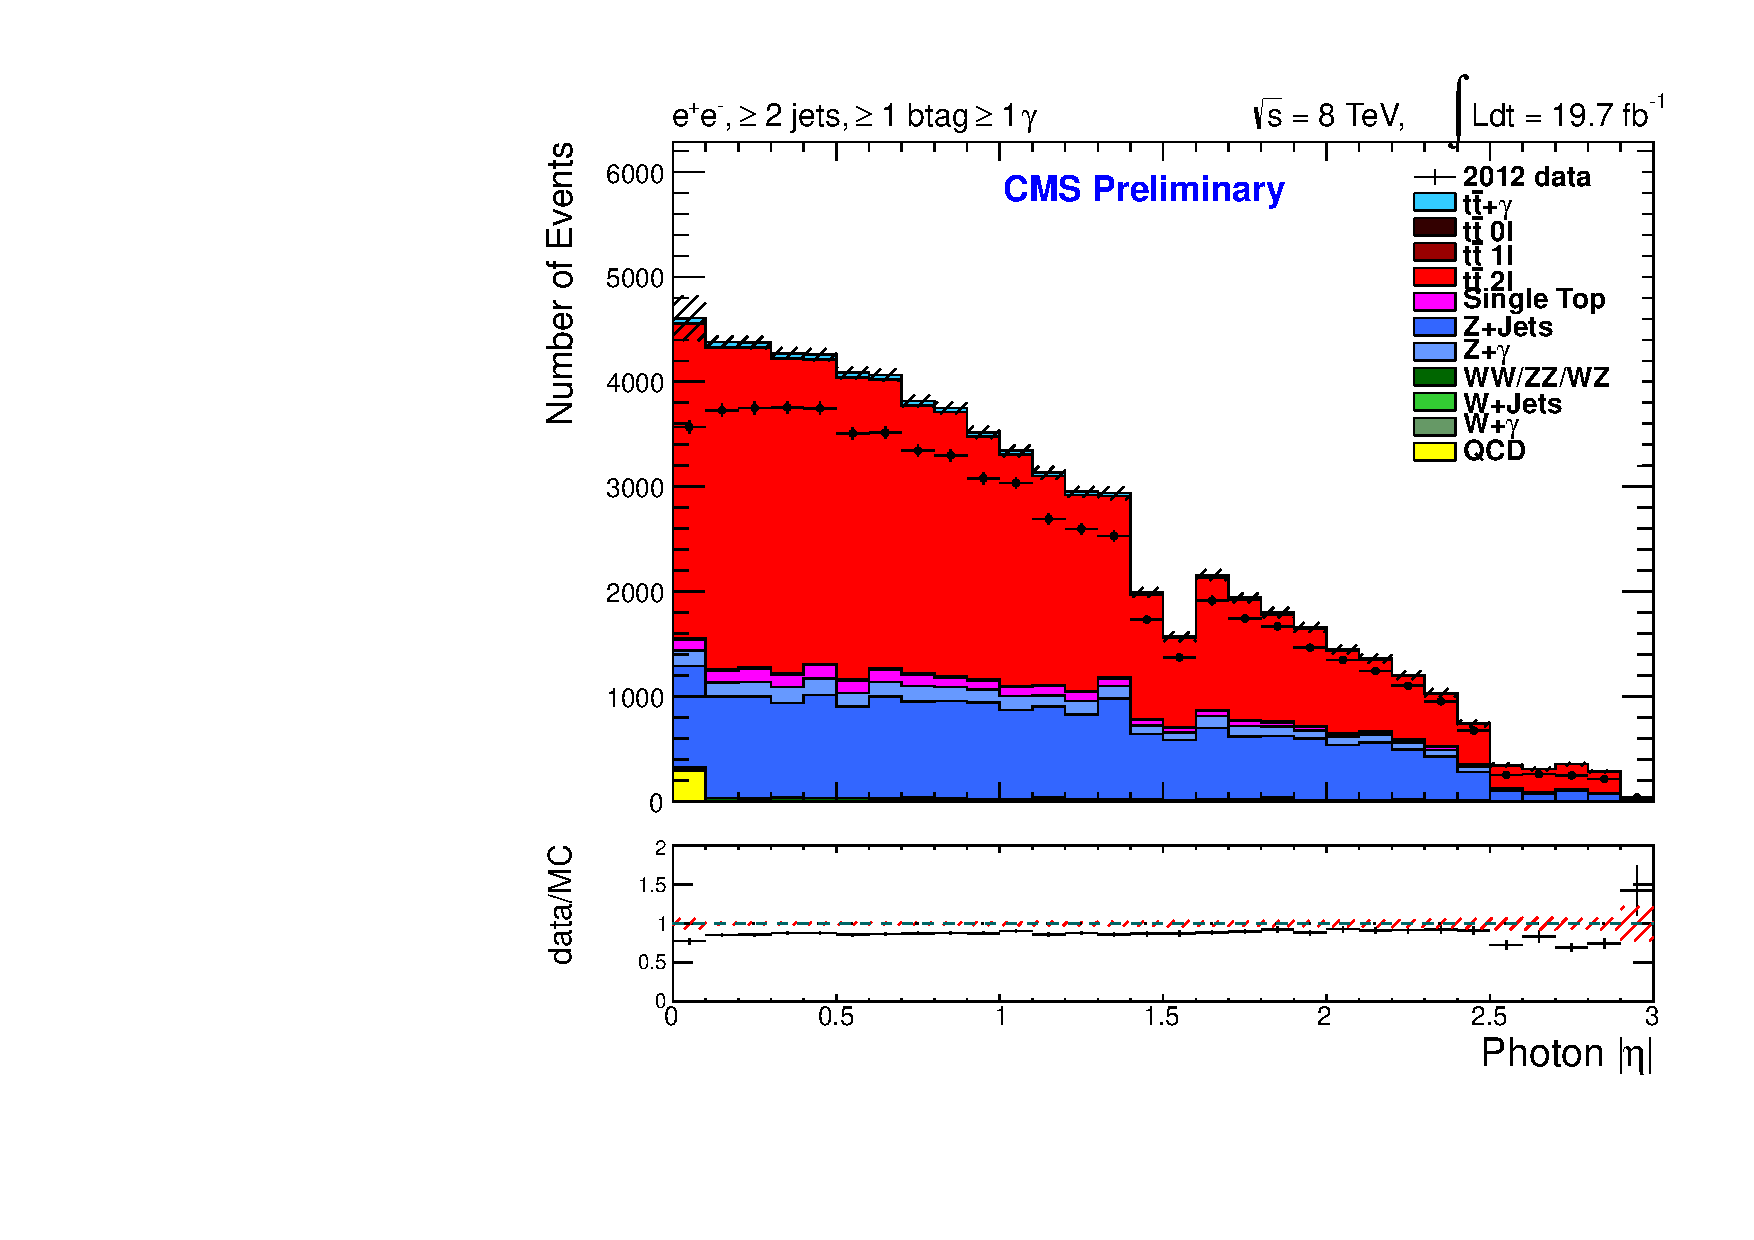
\includegraphics[width=0.5\textwidth]{Plots/ControlPlots/TTbarDiLeptonAnalysis/EE/Photons/AllPhotons/Photon_AbsEta_splitTTbar_ratio.pdf}\\
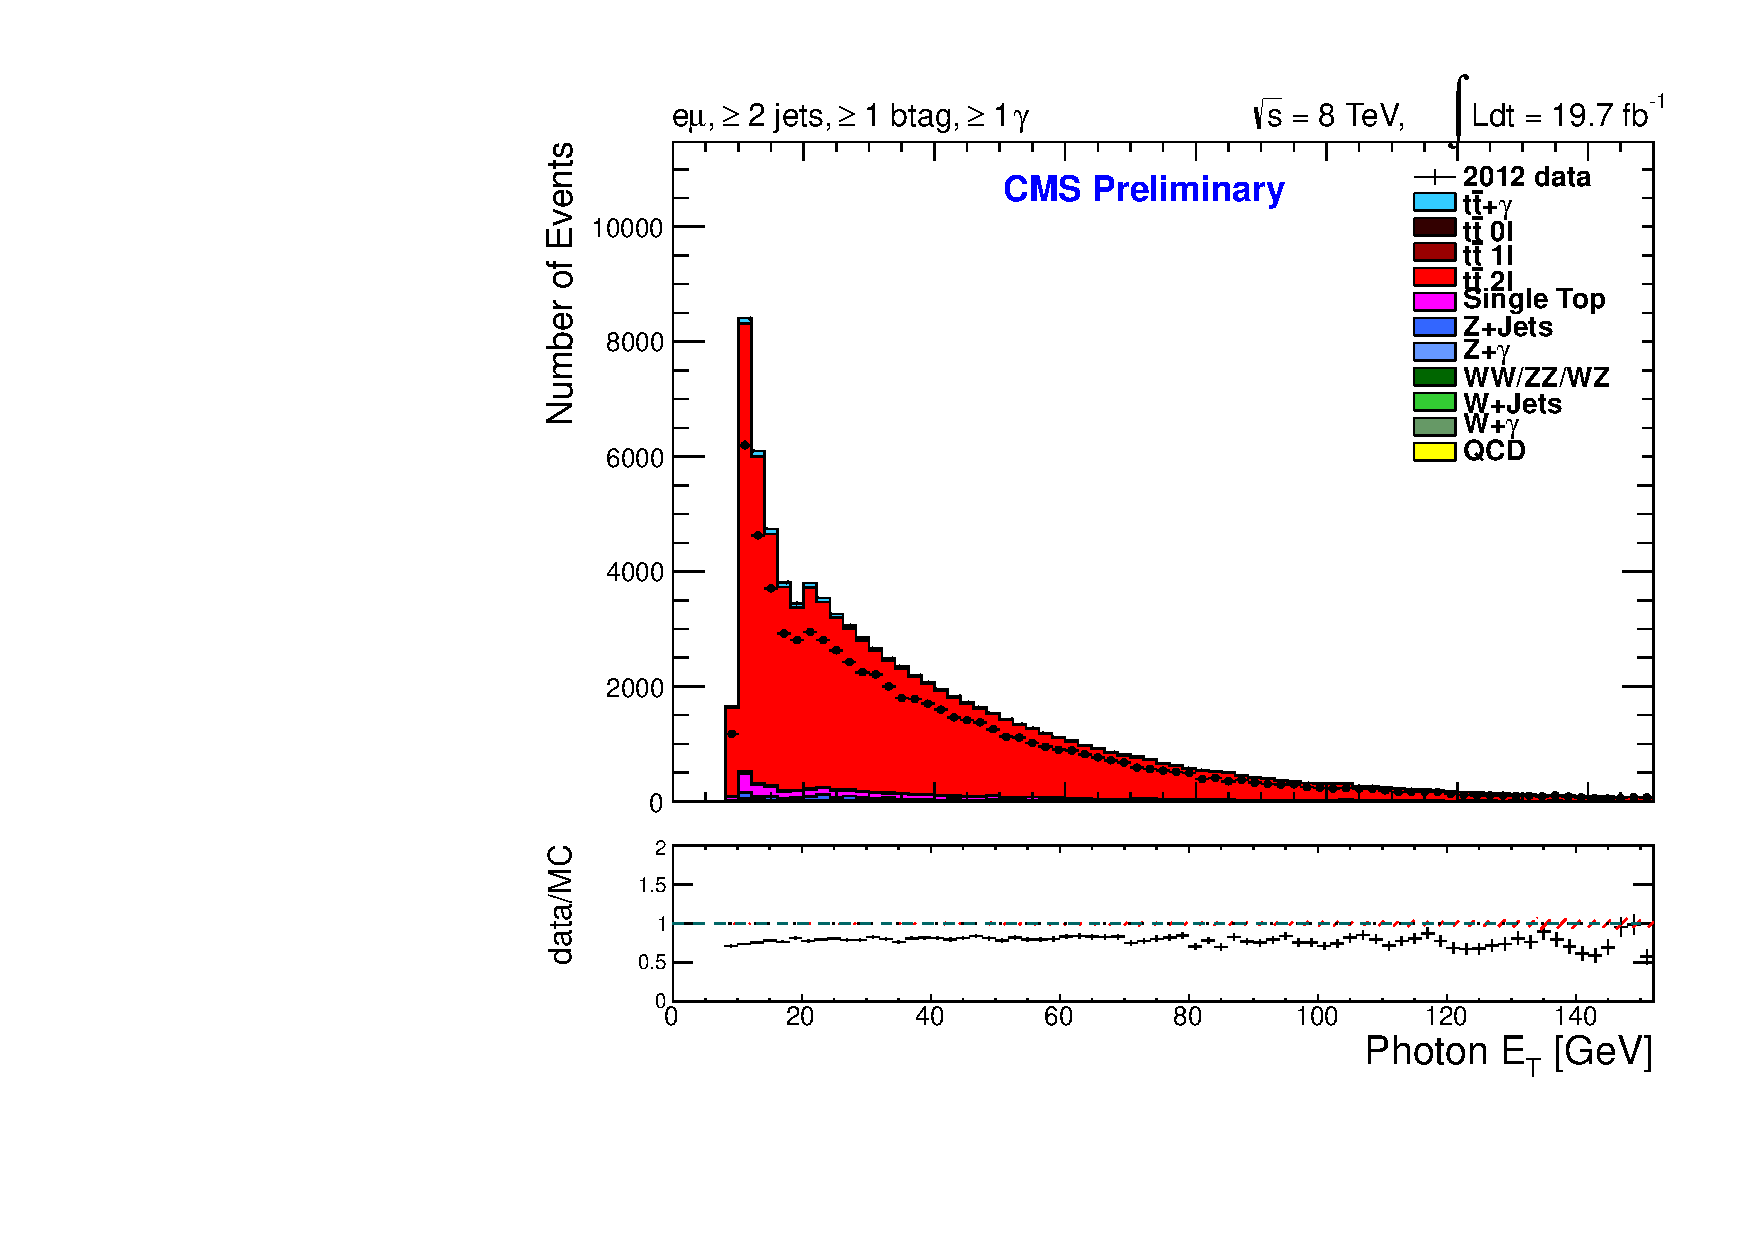
\includegraphics[width=0.5\textwidth]{Plots/ControlPlots/TTbarDiLeptonAnalysis/EMu/Photons/AllPhotons/Photon_ET_splitTTbar_ratio.pdf}
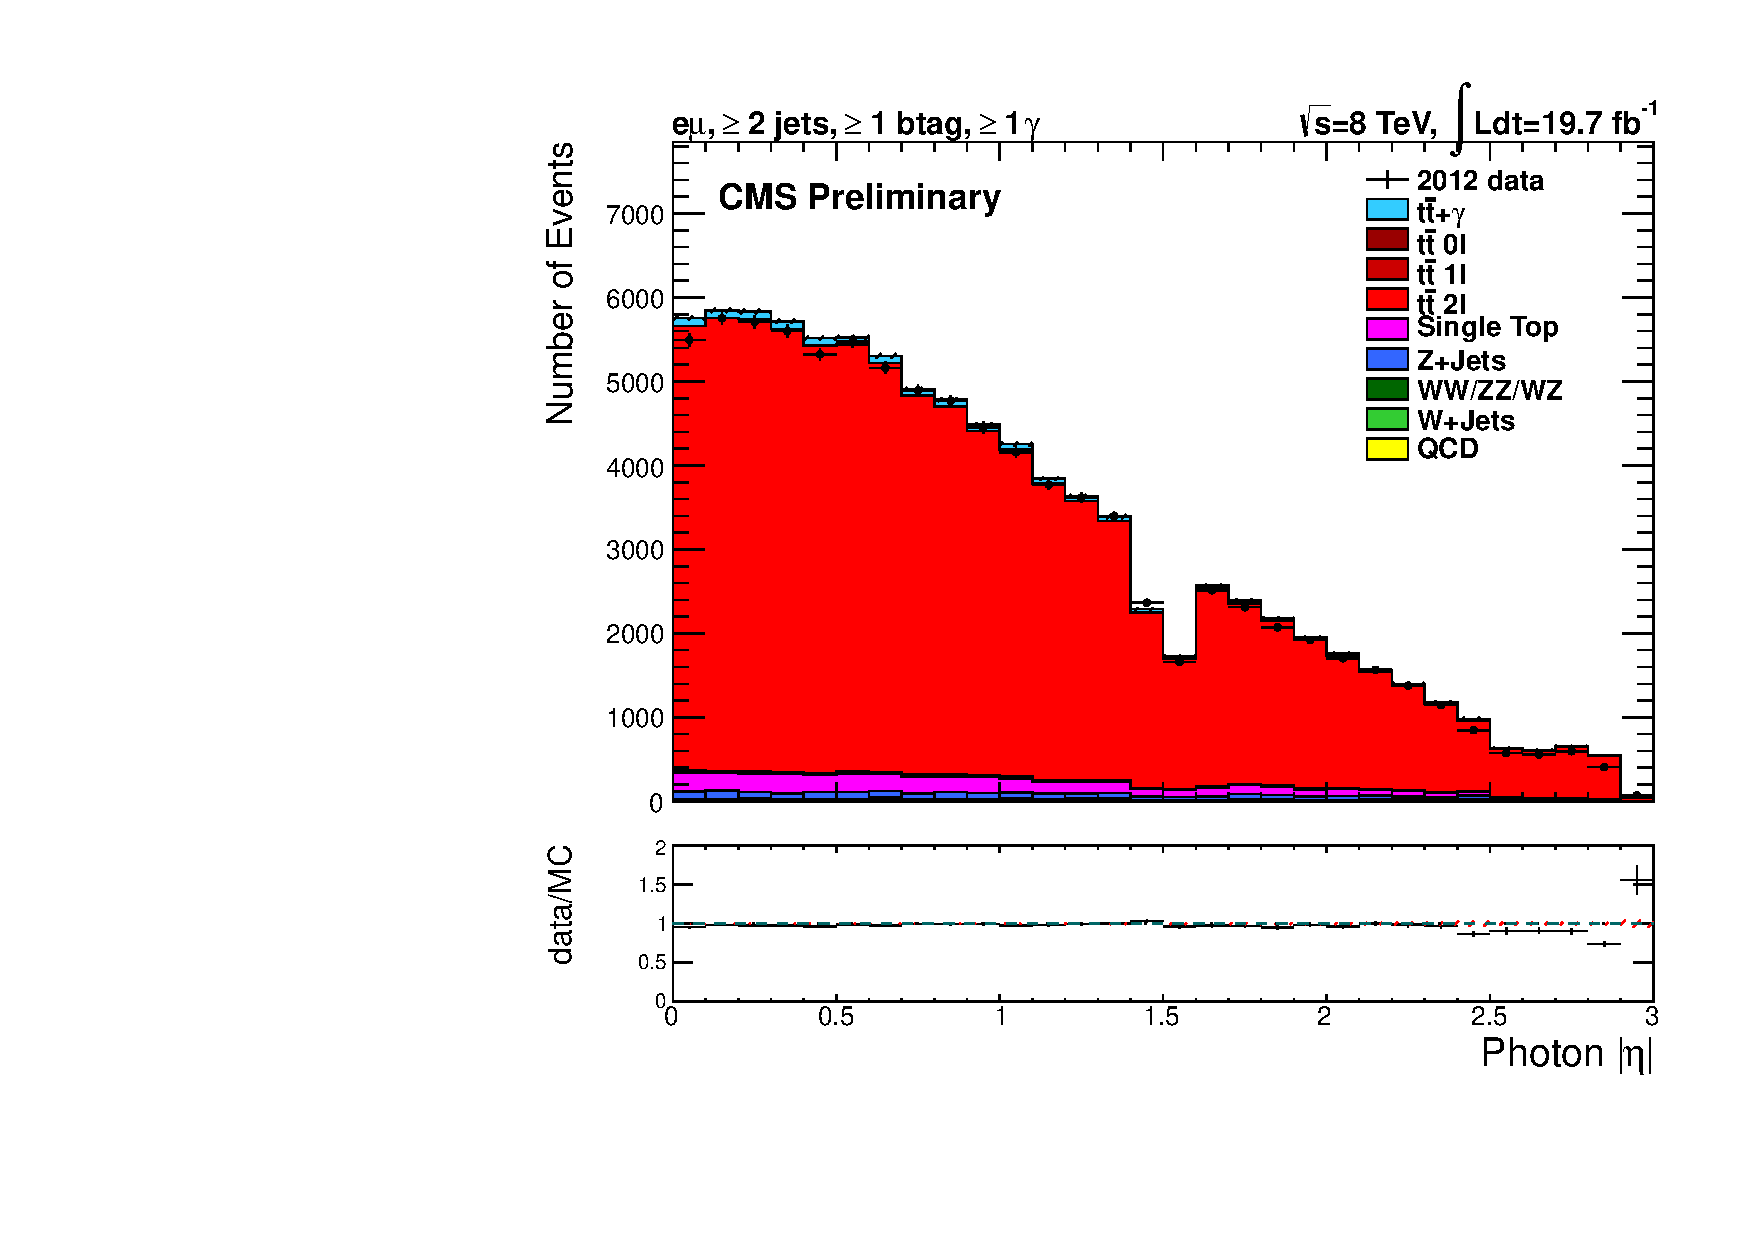
\includegraphics[width=0.5\textwidth]{Plots/ControlPlots/TTbarDiLeptonAnalysis/EMu/Photons/AllPhotons/Photon_AbsEta_splitTTbar_ratio.pdf}
\caption{Comparison of the E$_{T}$ and $|\eta|$ distributions in data and simulation in the $\mu^{+}\mu^{-}$, $e^{+}e^{-}$, and $e\mu$ channels after $t\bar{t}$ selection.}
\label{fig-ttbarETandEta}
\end{figure}

The distributions for the other variables can be seen in Figure \ref{fig-ttbarPlots}.

\begin{figure} 
%\begin{center}
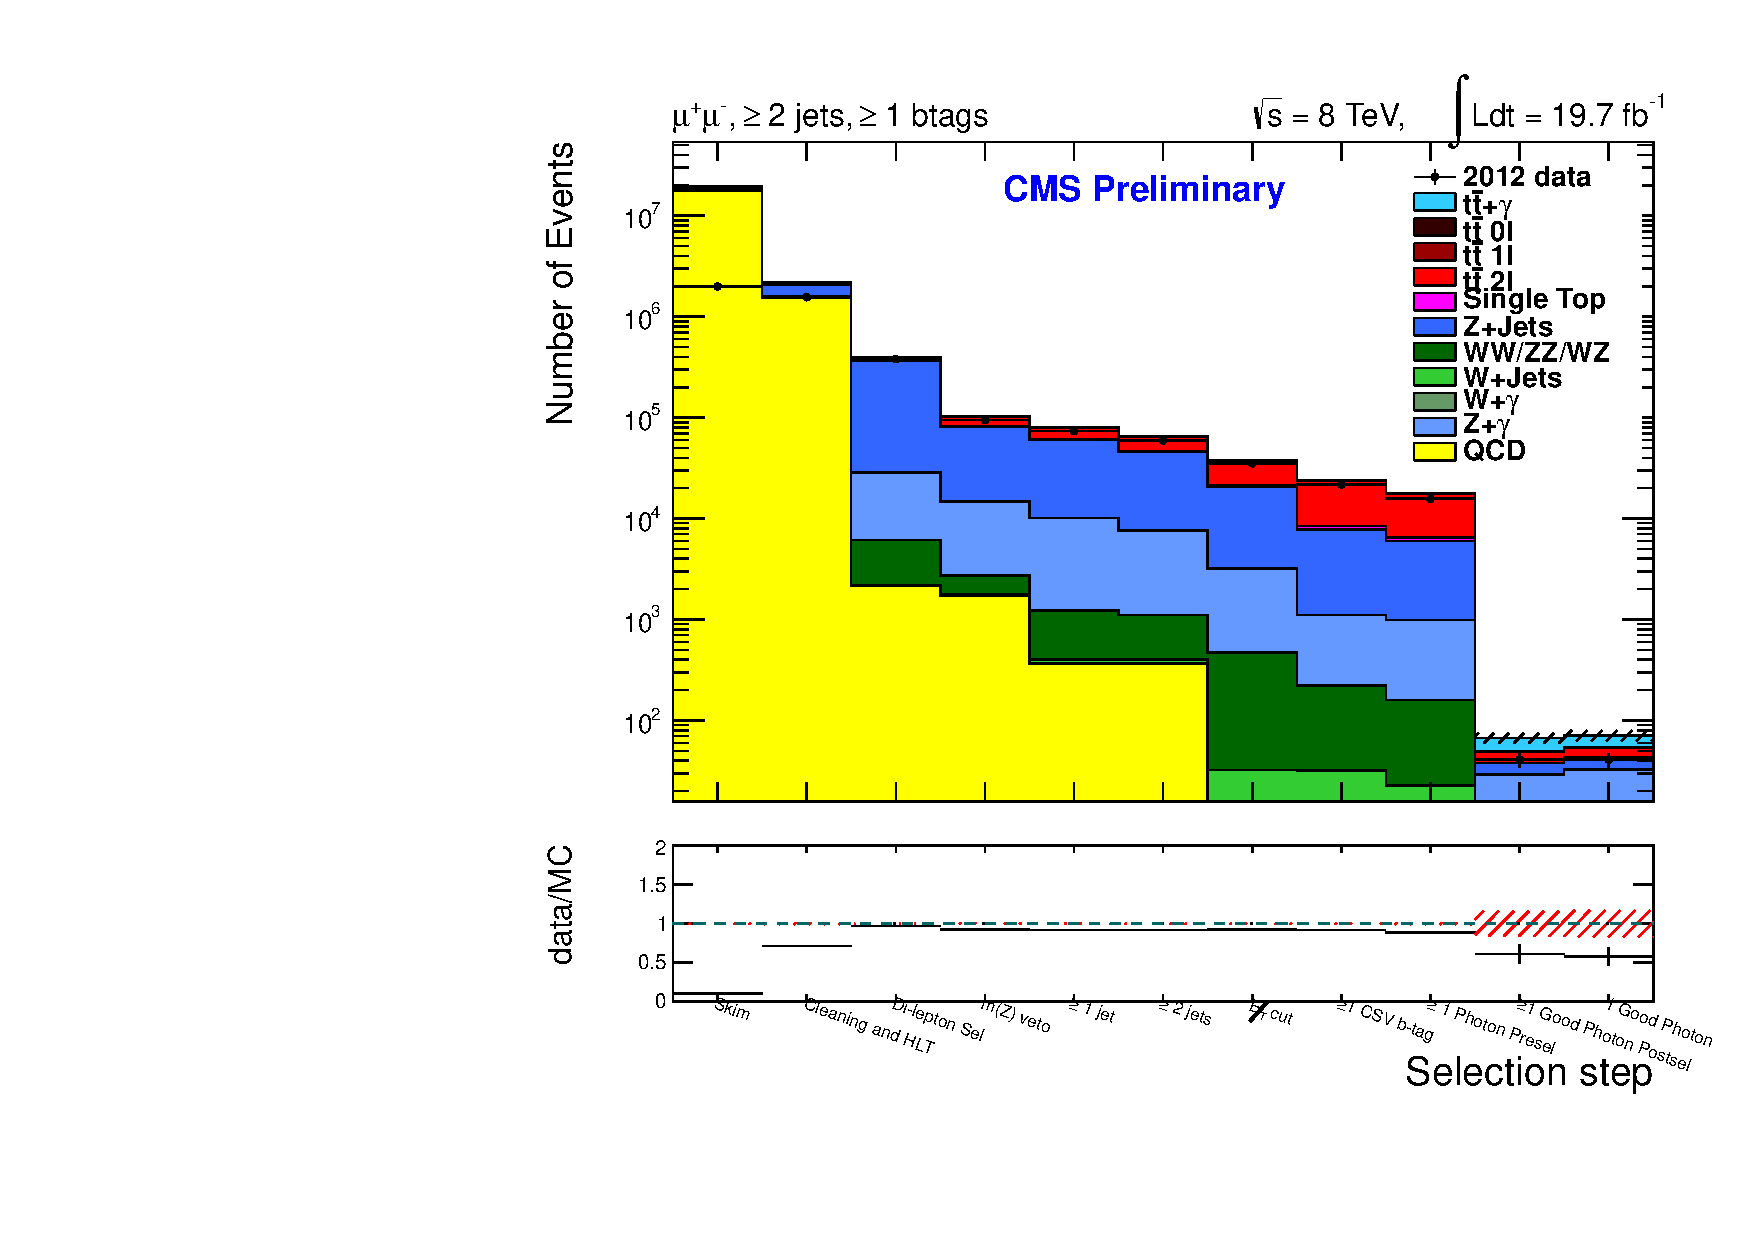
\includegraphics[width=0.5\textwidth]{Plots/ControlPlots/CutFlow/Log/TTbarMuMuRefSelection_splitTTbar_ratio.pdf}
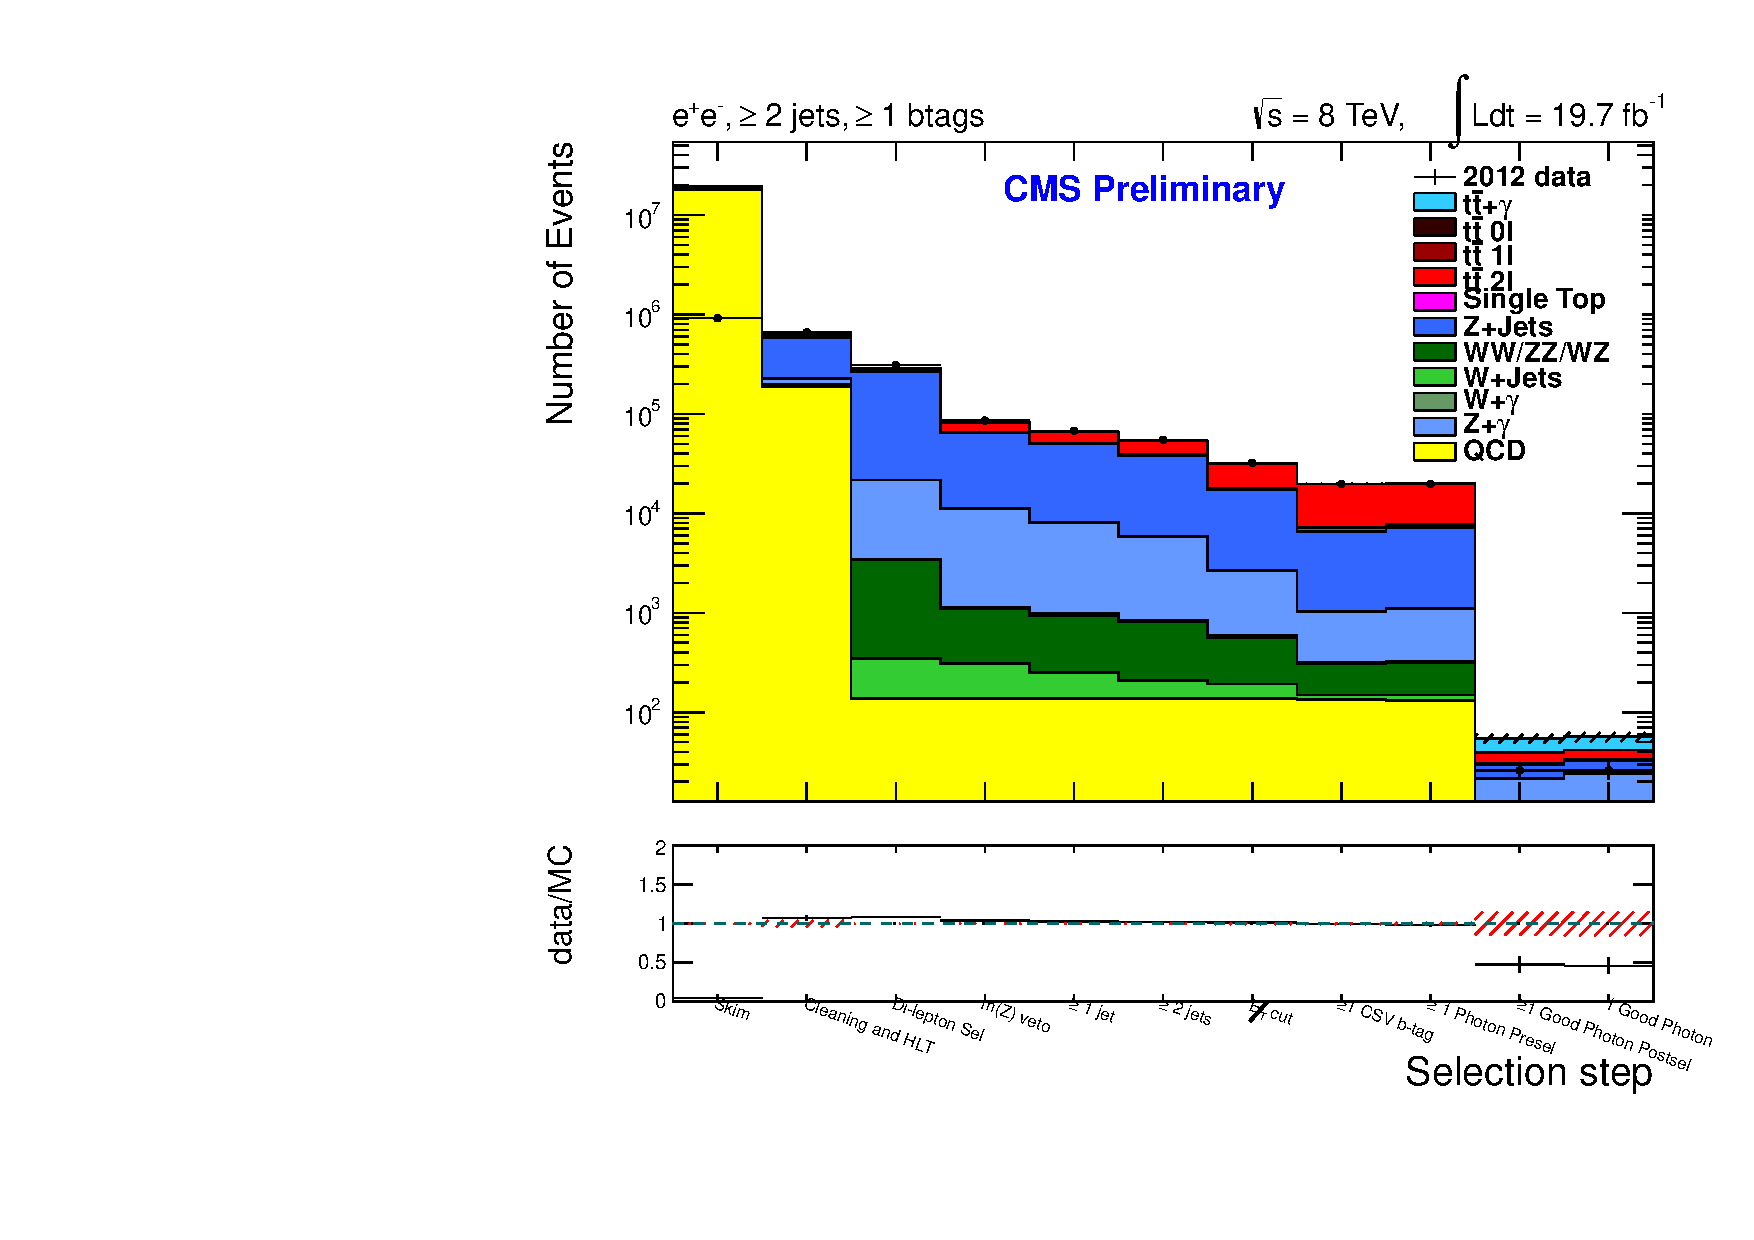
\includegraphics[width=0.5\textwidth]{Plots/ControlPlots/CutFlow/Log/TTbarEERefSelection_splitTTbar_ratio.pdf} \\
\begin{center}
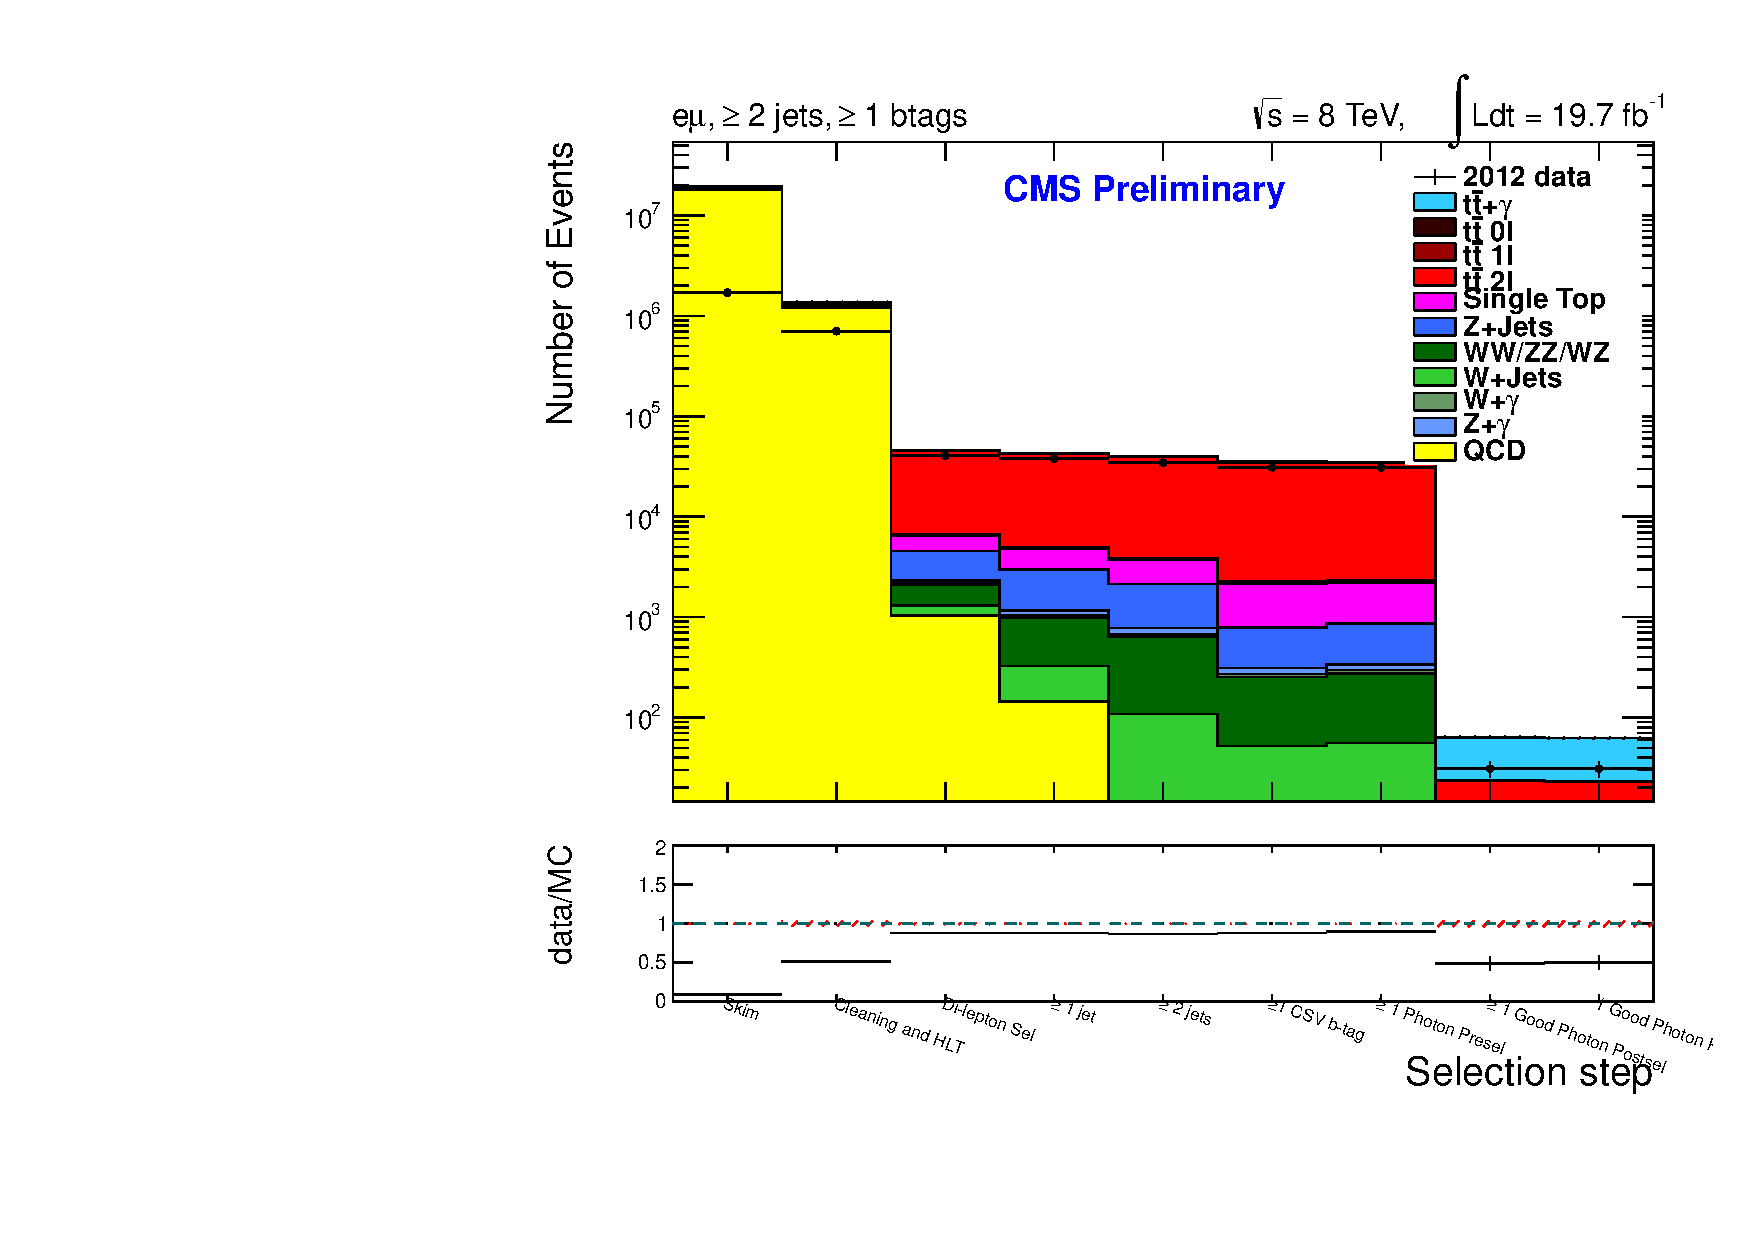
\includegraphics[width=0.5\textwidth]{Plots/ControlPlots/CutFlow/Log/TTbarEMuRefSelection_splitTTbar_ratio.pdf}
\end{center}
\caption{Cutflow plots showing the number of events remaining after individual cuts are introduced, comparing distributions in data and simulation in the $\mu^{+}\mu^{-}$, $e^{+}e^{-}$, and $e\mu$ channels.}
\label{fig-CutFlow}
\end{figure}

\begin{sidewaystable}
  \centering 
%  \caption{Cut Flow table for the $\mu^+\mu^-$ selection.}
%  \label{tab:mumu_cutflow}
\resizebox{\columnwidth}{!} {

\begin{tabular}{|l|l|l|l|l|l|l|l|l|l|l|l|}
\hline
\multicolumn{12}{|c|}{\textbf{Cut Flow table for the $\mu^+\mu^-$ selection}} \\
\hline
& \textbf{ttgamma} & \textbf{ttbar 0l} & \textbf{ttbar 1l} & \textbf{ttbar 2l} & \textbf{wjets} & \textbf{zjets} & \textbf{diboson} & \textbf{single t} & \textbf{qcd} & \textbf{all MC} & \textbf{data} \\
\hline
Skim & 3650 $\pm$ 12 \ & 18015 $\pm$ 38 \ & 141668 $\pm$ 117 \ & 147272 $\pm$ 84 \ & 213643 $\pm$ 1763 \ & 1318833 $\pm$ 1868 \ & 16881 $\pm$ 33 \ & 33315 $\pm$ 365 \ & 21035073 $\pm$ 153027\ & 22928349 $\pm$ 153049 \ & 2413504 $\pm$ 1554 \\
Cleaning and HLT & 1018 $\pm$ 6 \ & 3117 $\pm$ 16 \ & 36105 $\pm$ 59 \ & 46211 $\pm$ 47 \ & 10348 $\pm$ 387 \ & 624329 $\pm$ 1273 \ & 5977 $\pm$ 17 \ & 8049 $\pm$ 176 \ & 1737634 $\pm$ 21436\ & 2472789 $\pm$ 21478 \ & 1887786 $\pm$ 1374 \\
Di-lepton Sel & 292 $\pm$ 3 \ & 0 $\pm$ 0 \ & 149 $\pm$ 4 \ & 21477 $\pm$ 31 \ & 47 $\pm$ 25 \ & 422524 $\pm$ 1027 \ & 4348 $\pm$ 14 \ & 1186 $\pm$ 24 \ & 2437 $\pm$ 605\ & 452461 $\pm$ 1193 \ & 459842 $\pm$ 678 \\
m(Z) veto & 262 $\pm$ 3 \ & 0 $\pm$ 0 \ & 126 $\pm$ 3 \ & 19169 $\pm$ 30 \ & 47 $\pm$ 25 \ & 82812 $\pm$ 489 \ & 1047 $\pm$ 8 \ & 1062 $\pm$ 23 \ & 2001 $\pm$ 559\ & 106525 $\pm$ 744 \ & 114102 $\pm$ 338 \\
$\geq$ 1 jet & 241 $\pm$ 3 \ & 0 $\pm$ 0 \ & 104 $\pm$ 3 \ & 18574 $\pm$ 29 \ & 32 $\pm$ 20 \ & 61503 $\pm$ 431 \ & 915 $\pm$ 8 \ & 1001 $\pm$ 22 \ & 368 $\pm$ 261\ & 82738 $\pm$ 506 \ & 88692 $\pm$ 298 \\
$\geq$ 2 jets & 210 $\pm$ 3 \ & 0 $\pm$ 0 \ & 64 $\pm$ 2 \ & 17585 $\pm$ 28 \ & 32 $\pm$ 20 \ & 47551 $\pm$ 379 \ & 772 $\pm$ 7 \ & 878 $\pm$ 21 \ & 368 $\pm$ 261\ & 67462 $\pm$ 462 \ & 71800 $\pm$ 268 \\
$\slash{E_{T}}$ cut & 196 $\pm$ 3 \ & 0 $\pm$ 0 \ & 59 $\pm$ 2 \ & 16468 $\pm$ 27 \ & 32 $\pm$ 20 \ & 21441 $\pm$ 253 \ & 483 $\pm$ 6 \ & 825 $\pm$ 20 \ & 0 $\pm$ 0\ & 39505 $\pm$ 256 \ & 42553 $\pm$ 206 \\
$\geq$ 1 CSV b-tag & 179 $\pm$ 3 \ & 0 $\pm$ 0 \ & 48 $\pm$ 2 \ & 15127 $\pm$ 26 \ & 32 $\pm$ 20 \ & 8246 $\pm$ 165 \ & 207 $\pm$ 4 \ & 721 $\pm$ 19 \ & 0 $\pm$ 0\ & 24559 $\pm$ 169 \ & 26478 $\pm$ 163 \\
$\geq$ 1 Photon Presel & 173 $\pm$ 3 \ & 0 $\pm$ 0 \ & 37 $\pm$ 2 \ & 11099 $\pm$ 22 \ & 23 $\pm$ 17 \ & 6217 $\pm$ 150 \ & 151 $\pm$ 4 \ & 497 $\pm$ 15 \ & 0 $\pm$ 0\ & 18198 $\pm$ 154 \ & 19105 $\pm$ 138 \\
$\geq$ 1 Good Photon Postsel & 17 $\pm$ 1 \ & 0 $\pm$ 0 \ & 0 $\pm$ 0 \ & 12 $\pm$ 1 \ & 0 $\pm$ 0 \ & 12 $\pm$ 6 \ & 1 $\pm$ 0 \ & 0 $\pm$ 0 \ & 0 $\pm$ 0\ & 41 $\pm$ 6 \ & 46 $\pm$ 7 \\
1 Good Photon Postsel & 17 $\pm$ 1 \ & 0 $\pm$ 0 \ & 0 $\pm$ 0 \ & 11 $\pm$ 1 \ & 0 $\pm$ 0 \ & 13 $\pm$ 7 \ & 1 $\pm$ 0 \ & 0 $\pm$ 0 \ & 0 $\pm$ 0\ & 43 $\pm$ 7 \ & 46 $\pm$ 7 \\

\hline
\end{tabular}
}
\caption{The number of expected events in MC and events observed in data for the $\mu^+\mu^-$ channel, before the fitting process, including statistical uncertainties.}
\end{sidewaystable}

\begin{sidewaystable}[h!]
  \centering
%  \caption{Cut Flow table for the  $e^+e^-$ selection.}
  %\label{tab:mumu_cutflow}
\resizebox{\columnwidth}{!} {

\begin{tabular}{|l|l|l|l|l|l|l|l|l|l|l|l|}
\hline
\multicolumn{12}{|c|}{\textbf{Cut Flow table for the $e^+e^-$ selection}} \\
\hline
& \textbf{ttgamma} & \textbf{ttbar 0l} & \textbf{ttbar 1l} & \textbf{ttbar 2l} & \textbf{wjets} & \textbf{zjets} & \textbf{diboson} & \textbf{single t} & \textbf{qcd} & \textbf{all MC} & \textbf{data} \\
\hline
Skim & 3632 $\pm$ 12 \ & 18015 $\pm$ 38 \ & 141660 $\pm$ 117 \ & 146469 $\pm$ 83 \ & 213610 $\pm$ 1763 \ & 1295804 $\pm$ 1838 \ & 16644 $\pm$ 33 \ & 33257 $\pm$ 365 \ & 21035139 $\pm$ 153027\ & 22904230 $\pm$ 153048 \ & 1137895 $\pm$ 1067 \\
Cleaning and HLT & 533 $\pm$ 5 \ & 142 $\pm$ 3 \ & 4302 $\pm$ 20 \ & 25215 $\pm$ 34 \ & 10504 $\pm$ 390 \ & 438516 $\pm$ 1038 \ & 4631 $\pm$ 15 \ & 2072 $\pm$ 66 \ & 206158 $\pm$ 19623\ & 692073 $\pm$ 19655 \ & 817968 $\pm$ 904 \\
Di-lepton Sel & 275 $\pm$ 3 \ & 0 $\pm$ 0 \ & 109 $\pm$ 3 \ & 17942 $\pm$ 28 \ & 299 $\pm$ 59 \ & 303836 $\pm$ 837 \ & 3389 $\pm$ 12 \ & 974 $\pm$ 22 \ & 257 $\pm$ 182\ & 327080 $\pm$ 860 \ & 384642 $\pm$ 620 \\
m(Z) veto & 247 $\pm$ 3 \ & 0 $\pm$ 0 \ & 93 $\pm$ 3 \ & 16018 $\pm$ 26 \ & 248 $\pm$ 54 \ & 66531 $\pm$ 418 \ & 852 $\pm$ 7 \ & 874 $\pm$ 21 \ & 257 $\pm$ 182\ & 85120 $\pm$ 460 \ & 106244 $\pm$ 326 \\
$\geq$ 1 jet & 220 $\pm$ 3 \ & 0 $\pm$ 0 \ & 85 $\pm$ 3 \ & 15296 $\pm$ 26 \ & 166 $\pm$ 44 \ & 51367 $\pm$ 375 \ & 757 $\pm$ 7 \ & 838 $\pm$ 21 \ & 257 $\pm$ 182\ & 68987 $\pm$ 420 \ & 83739 $\pm$ 289 \\
$\geq$ 2 jets & 188 $\pm$ 3 \ & 0 $\pm$ 0 \ & 72 $\pm$ 2 \ & 14501 $\pm$ 25 \ & 97 $\pm$ 34 \ & 40075 $\pm$ 332 \ & 654 $\pm$ 6 \ & 754 $\pm$ 19 \ & 137 $\pm$ 137\ & 56478 $\pm$ 362 \ & 67769 $\pm$ 260 \\
$\slash{E_{T}}$ cut & 175 $\pm$ 3 \ & 0 $\pm$ 0 \ & 65 $\pm$ 2 \ & 13596 $\pm$ 24 \ & 81 $\pm$ 31 \ & 18112 $\pm$ 220 \ & 407 $\pm$ 5 \ & 701 $\pm$ 18 \ & 137 $\pm$ 137\ & 33274 $\pm$ 263 \ & 39949 $\pm$ 200 \\
$\geq$ 1 CSV b-tag & 161 $\pm$ 2 \ & 0 $\pm$ 0 \ & 55 $\pm$ 2 \ & 12487 $\pm$ 23 \ & 29 $\pm$ 21 \ & 6826 $\pm$ 142 \ & 170 $\pm$ 3 \ & 601 $\pm$ 17 \ & 134 $\pm$ 134\ & 20463 $\pm$ 198 \ & 24449 $\pm$ 156 \\
$\geq$ 1 Photon Presel & 157 $\pm$ 2 \ & 0 $\pm$ 0 \ & 53 $\pm$ 2 \ & 12213 $\pm$ 23 \ & 34 $\pm$ 24 \ & 7433 $\pm$ 156 \ & 182 $\pm$ 4 \ & 585 $\pm$ 16 \ & 131 $\pm$ 131\ & 20790 $\pm$ 207 \ & 24449 $\pm$ 156 \\
$\geq$ 1 Good Photon Postsel & 15 $\pm$ 1 \ & 0 $\pm$ 0 \ & 0 $\pm$ 0 \ & 9 $\pm$ 1 \ & 0 $\pm$ 0 \ & 12 $\pm$ 5 \ & 0 $\pm$ 0 \ & 1 $\pm$ 1 \ & 0 $\pm$ 0\ & 37 $\pm$ 5 \ & 34 $\pm$ 6 \\
1 Good Photon Postsel & 15 $\pm$ 1 \ & 0 $\pm$ 0 \ & 0 $\pm$ 0 \ & 9 $\pm$ 1 \ & 0 $\pm$ 0 \ & 12 $\pm$ 5 \ & 1 $\pm$ 0 \ & 1 $\pm$ 0 \ & 0 $\pm$ 0\ & 37 $\pm$ 5 \ & 34 $\pm$ 6 \\

\hline
\end{tabular}
}
\caption{The number of expected events in MC and events observed in data for the $e^+e^-$ channel, before the fitting process, including statistical uncertainties.}
\end{sidewaystable}

\begin{sidewaystable}[h!]
  \centering
%  \caption{Cut Flow table for the e \mu$ selection.}
%  \label{tab:mumu_cutflow}
\resizebox{\columnwidth}{!} {

\begin{tabular}{|l|l|l|l|l|l|l|l|l|l|l|l|}
\hline
\multicolumn{12}{|c|}{\textbf{Cut Flow table for the e$\mu$ selection}} \\
\hline
& \textbf{ttgamma} & \textbf{ttbar 0l} & \textbf{ttbar 1l} & \textbf{ttbar 2l} & \textbf{wjets} & \textbf{zjets} & \textbf{diboson} & \textbf{single t} & \textbf{qcd} & \textbf{all MC} & \textbf{data} \\
\hline
Skim & 3610 $\pm$ 12 \ & 18015 $\pm$ 38 \ & 141648 $\pm$ 117 \ & 144829 $\pm$ 82 \ & 213614 $\pm$ 1763 \ & 1334209 $\pm$ 1889 \ & 16963 $\pm$ 33 \ & 33168 $\pm$ 365 \ & 21035027 $\pm$ 153027 \ & 22941082 $\pm$ 153049\ & 2125311 $\pm$ 1458 \\
Cleaning and HLT & 1407 $\pm$ 8 \ & 1147 $\pm$ 10 \ & 34466 $\pm$ 58 \ & 63666 $\pm$ 54 \ & 22308 $\pm$ 570 \ & 28157 $\pm$ 277 \ & 2018 $\pm$ 14 \ & 8624 $\pm$ 167 \ & 1410492 $\pm$ 34863 \ & 1572284 $\pm$ 34869\ & 875176 $\pm$ 936 \\
Di-lepton Sel & 560 $\pm$ 5 \ & 0 $\pm$ 0 \ & 261 $\pm$ 5 \ & 38902 $\pm$ 41 \ & 313 $\pm$ 62 \ & 2776 $\pm$ 80 \ & 852 $\pm$ 9 \ & 2114 $\pm$ 35 \ & 1301 $\pm$ 406 \ & 47079 $\pm$ 422\ & 50564 $\pm$ 225 \\
$\geq$ 1 jet & 508 $\pm$ 4 \ & 0 $\pm$ 0 \ & 226 $\pm$ 4 \ & 37416 $\pm$ 41 \ & 230 $\pm$ 53 \ & 2253 $\pm$ 73 \ & 713 $\pm$ 8 \ & 2009 $\pm$ 35 \ & 145 $\pm$ 131 \ & 43499 $\pm$ 168\ & 47188 $\pm$ 217 \\
$\geq$ 2 jets & 440 $\pm$ 4 \ & 0 $\pm$ 0 \ & 172 $\pm$ 4 \ & 35445 $\pm$ 40 \ & 157 $\pm$ 43 \ & 1676 $\pm$ 63 \ & 572 $\pm$ 8 \ & 1767 $\pm$ 29 \ & 0 $\pm$ 0 \ & 40230 $\pm$ 91\ & 43107 $\pm$ 208 \\
$\geq$ 1 CSV b-tag & 404 $\pm$ 4 \ & 0 $\pm$ 0 \ & 142 $\pm$ 3 \ & 32569 $\pm$ 38 \ & 90 $\pm$ 34 \ & 622 $\pm$ 39 \ & 219 $\pm$ 5 \ & 1529 $\pm$ 27 \ & 0 $\pm$ 0 \ & 35575 $\pm$ 70\ & 38657 $\pm$ 197 \\
$\geq$ 1 Photon Presel & 395 $\pm$ 4 \ & 0 $\pm$ 0 \ & 139 $\pm$ 3 \ & 31855 $\pm$ 37 \ & 98 $\pm$ 37 \ & 676 $\pm$ 43 \ & 239 $\pm$ 5 \ & 1490 $\pm$ 26 \ & 0 $\pm$ 0 \ & 34891 $\pm$ 73\ & 38657 $\pm$ 197 \\
$\geq$ 1 Good Photon Postsel & 40 $\pm$ 1 \ & 0 $\pm$ 0 \ & 0 $\pm$ 0 \ & 23 $\pm$ 1 \ & 0 $\pm$ 0 \ & 0 $\pm$ 0 \ & 0 $\pm$ 0 \ & 1 $\pm$ 1 \ & 0 $\pm$ 0 \ & 64 $\pm$ 2\ & 42 $\pm$ 6 \\
1 Good Photon Postsel & 39 $\pm$ 1 \ & 0 $\pm$ 0 \ & 0 $\pm$ 0 \ & 22 $\pm$ 1 \ & 0 $\pm$ 0 \ & 0 $\pm$ 0 \ & 0 $\pm$ 0 \ & 1 $\pm$ 1 \ & 0 $\pm$ 0 \ & 62 $\pm$ 2\ & 41 $\pm$ 6 \\

\hline
\end{tabular}
}
\caption{The number of expected events in MC and events observed in data for the $e\mu$ channel, before the fitting process, including statistical uncertainties.}
\end{sidewaystable}

% \begin{figure}
% \begin{center}
% \includegraphics[width=0.5\textwidth]{Plots/}\includegraphics[width=0.5\textwidth]{Plots/}
% \includegraphics[width=0.5\textwidth]{Plots/}\includegraphics[width=0.5\textwidth]{Plots/}
% \end{center}
% \caption{}
% \end{figure}

\section{Selection of $t\bar{t}+\gamma$ events} \label{sec-postselection}

From the set of $t\bar{t}$ preselected events in Section \ref{sec-Preselection}, we select only events with a photon candidate present.  Fiducial requirements are implemented as cuts in $\abs{\eta}$ and $E_T$. CMS recommended cuts are added for fiducialisation and photon selection (loose cut-based photon ID 2012 with particle flow based isolation, \cite{CutBasedIsolation2012}).In order to suppress FSR from final state particles a $\Delta R$ cut of photons between jets and leptons is applied. All simulated data is scaled to the luminosity of the recorded data used.  

The fiducial cuts on the photon are given as:

\begin{description}

\item[Transverse energy] A transverse energy cut of $E_T > 25$ is implemented in order to suppress the numerous low energy fake photons and photons from other vertices other than the primary
vertex. The transverse energy distribution for each decay channel can be seen in Figure.\ref{fig-photonSelectionETandEta}.

\item[Pseudorapidity] An acceptance cut on the fiducial region of just the CMS ECAL barrel (EB), $\abs{\eta} < 1.4442$, is applied to verify that the electromagnetic shower of the photon will be fully reconstructed. We will not be including the ECAL Endcap (EE) in this analysis due to the difficulty in identifying a photon thus giving very low statistics.

\end{description}

The fiducial variable distributions are shown in Figure \ref{fig-photonSelectionETandEta}.

\begin{figure}
% \begin{center}
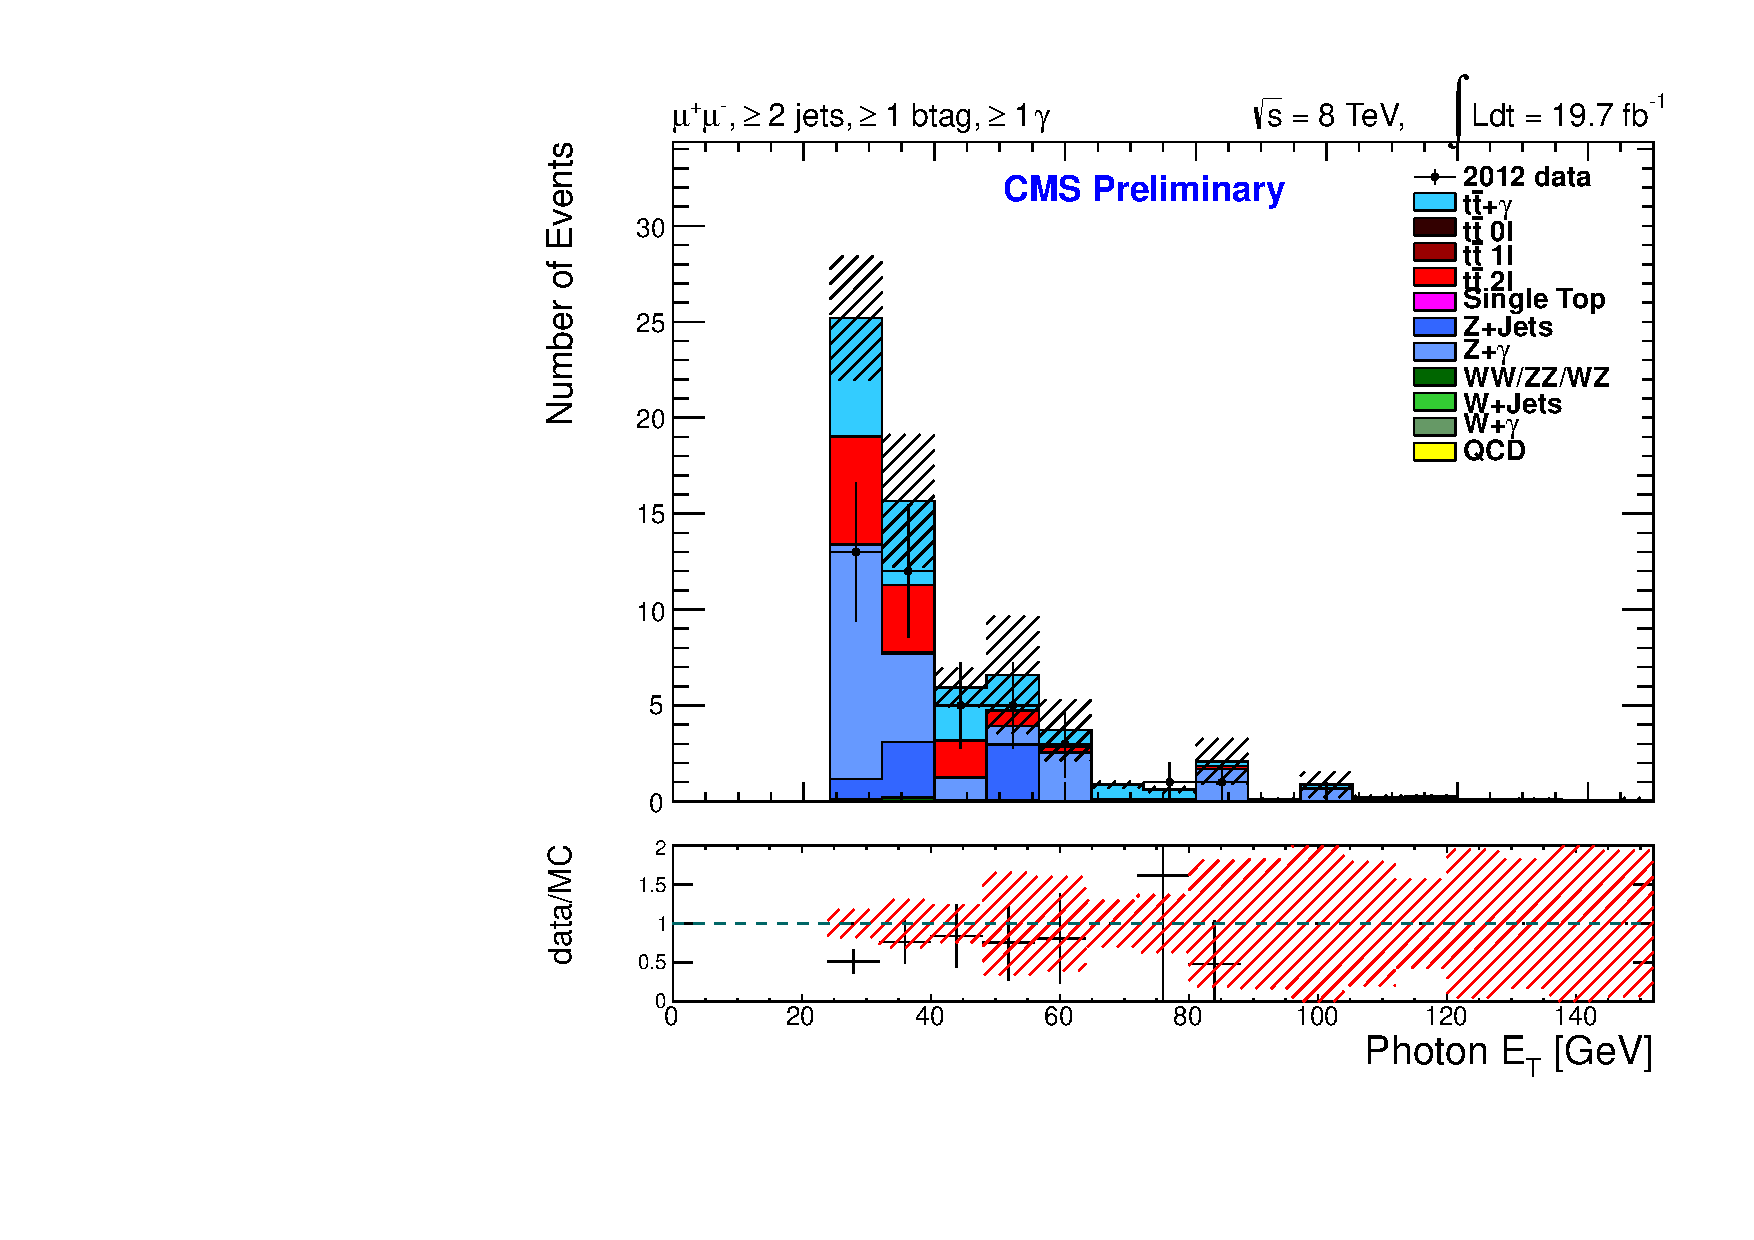
\includegraphics[width=0.5\textwidth]{Plots/ControlPlots/TTbarPhotonAnalysis/MuMu/Photons/SignalPhotons/Photon_ET_splitTTbar_ratio.pdf}
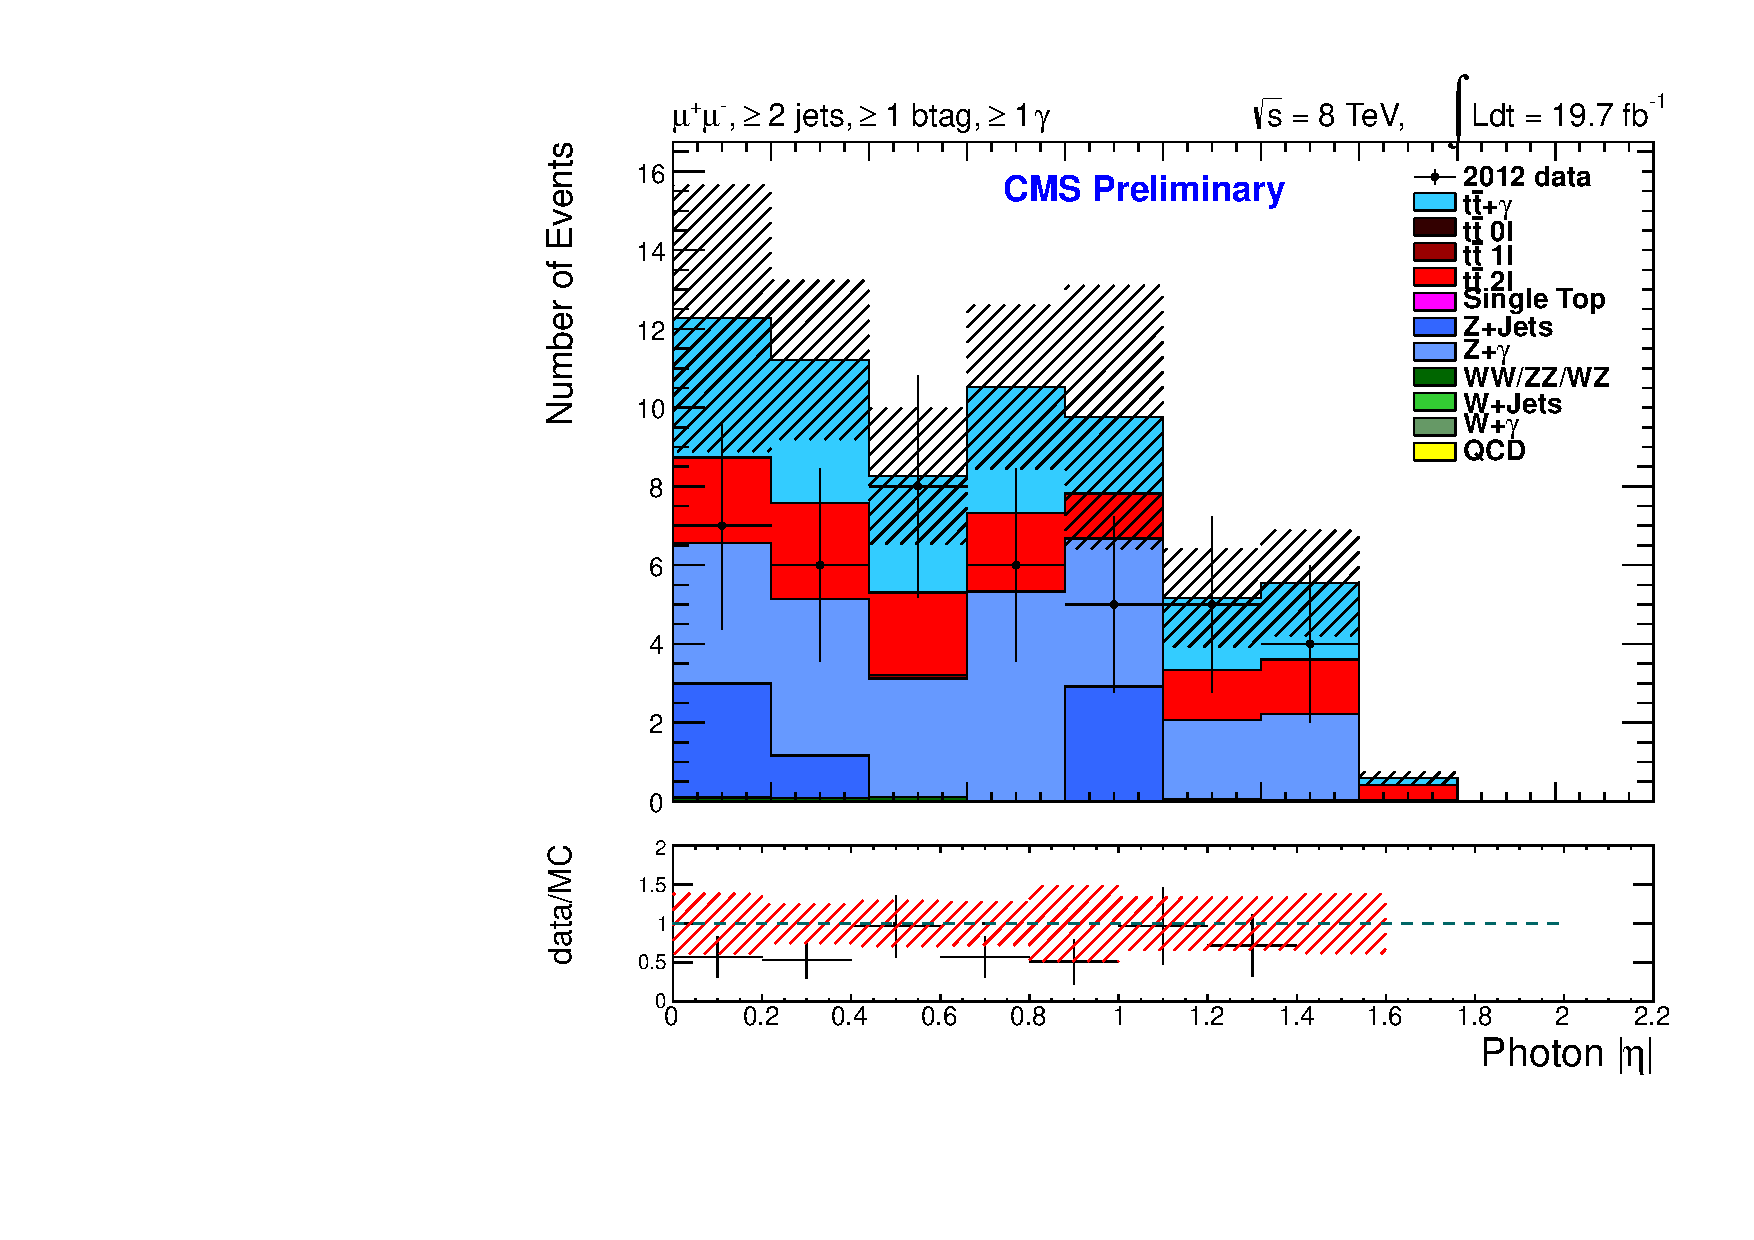
\includegraphics[width=0.5\textwidth]{Plots/ControlPlots/TTbarPhotonAnalysis/MuMu/Photons/SignalPhotons/Photon_AbsEta_splitTTbar_ratio.pdf} \\
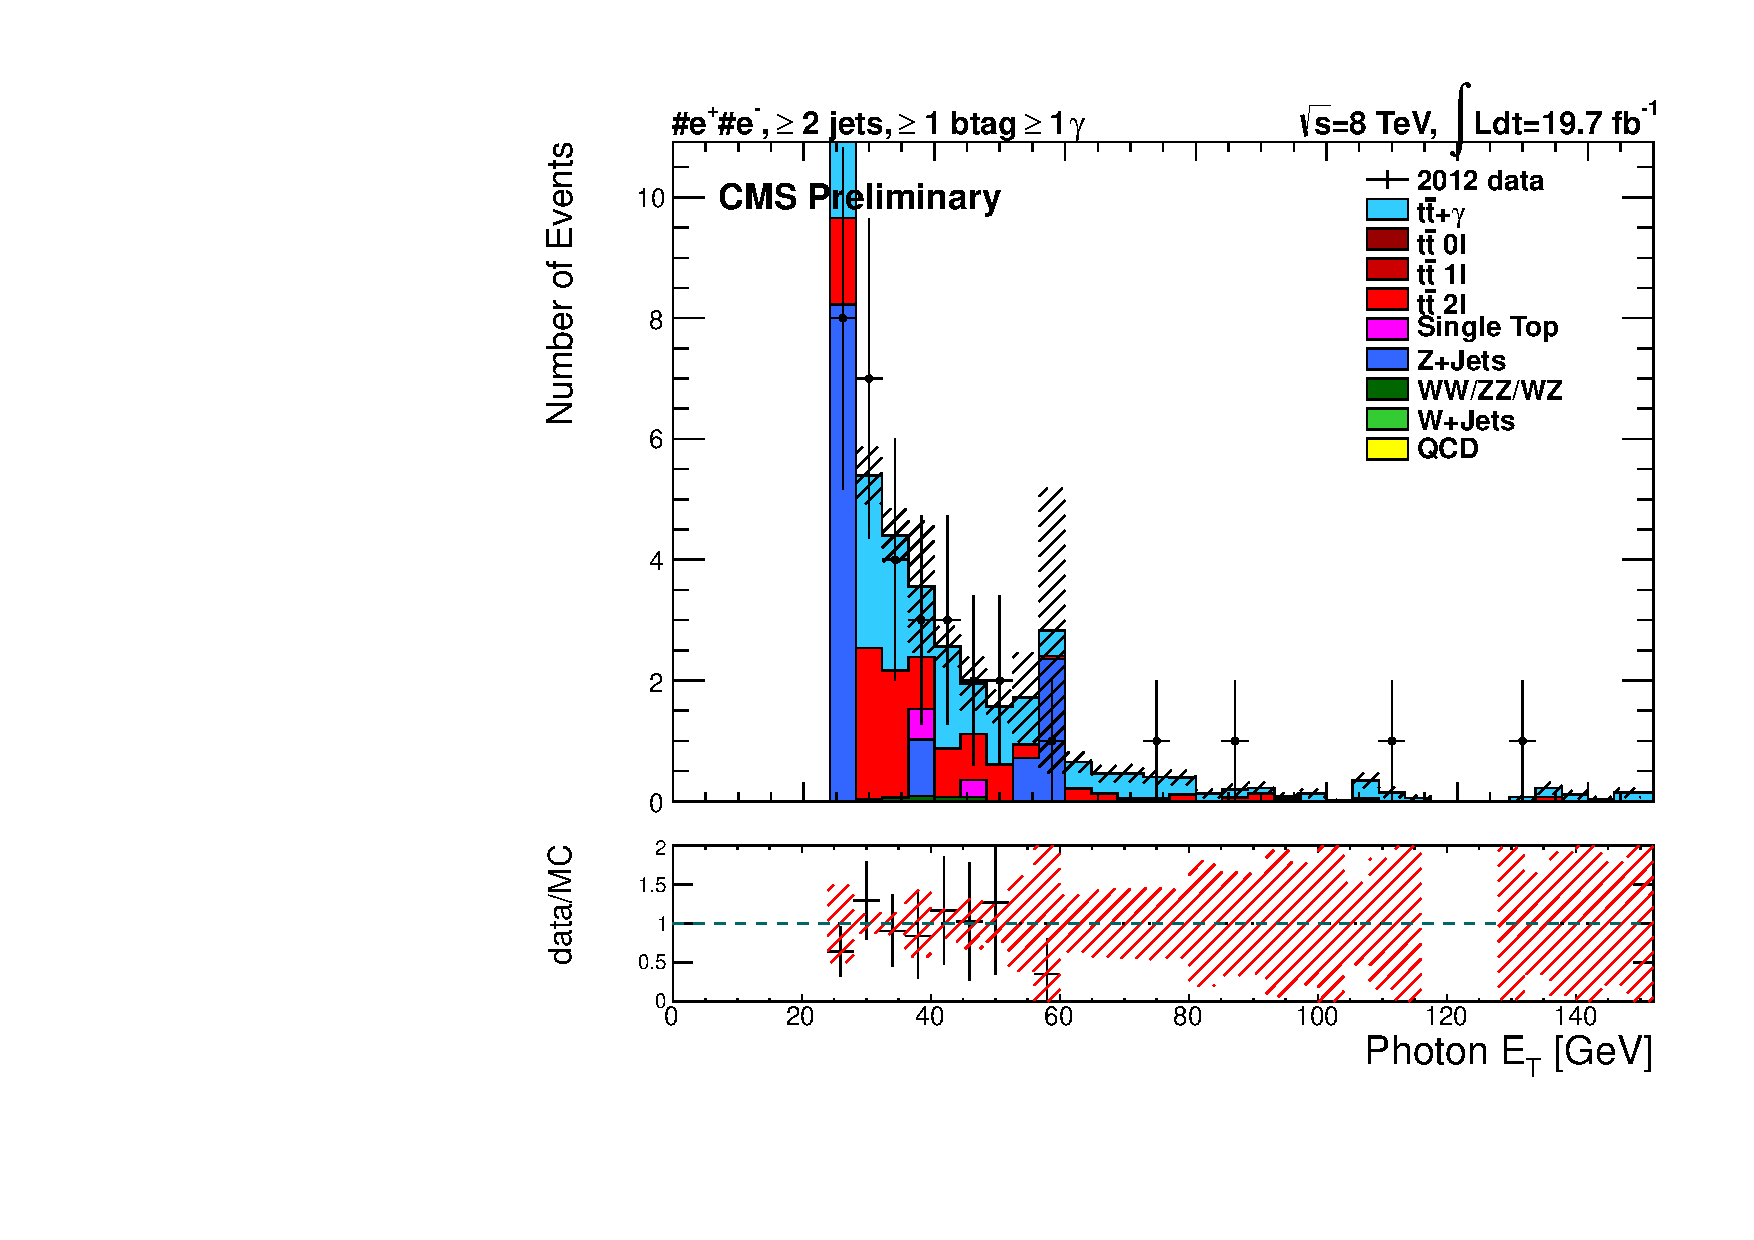
\includegraphics[width=0.5\textwidth]{Plots/ControlPlots/TTbarPhotonAnalysis/EE/Photons/SignalPhotons/Photon_ET_splitTTbar_ratio.pdf}
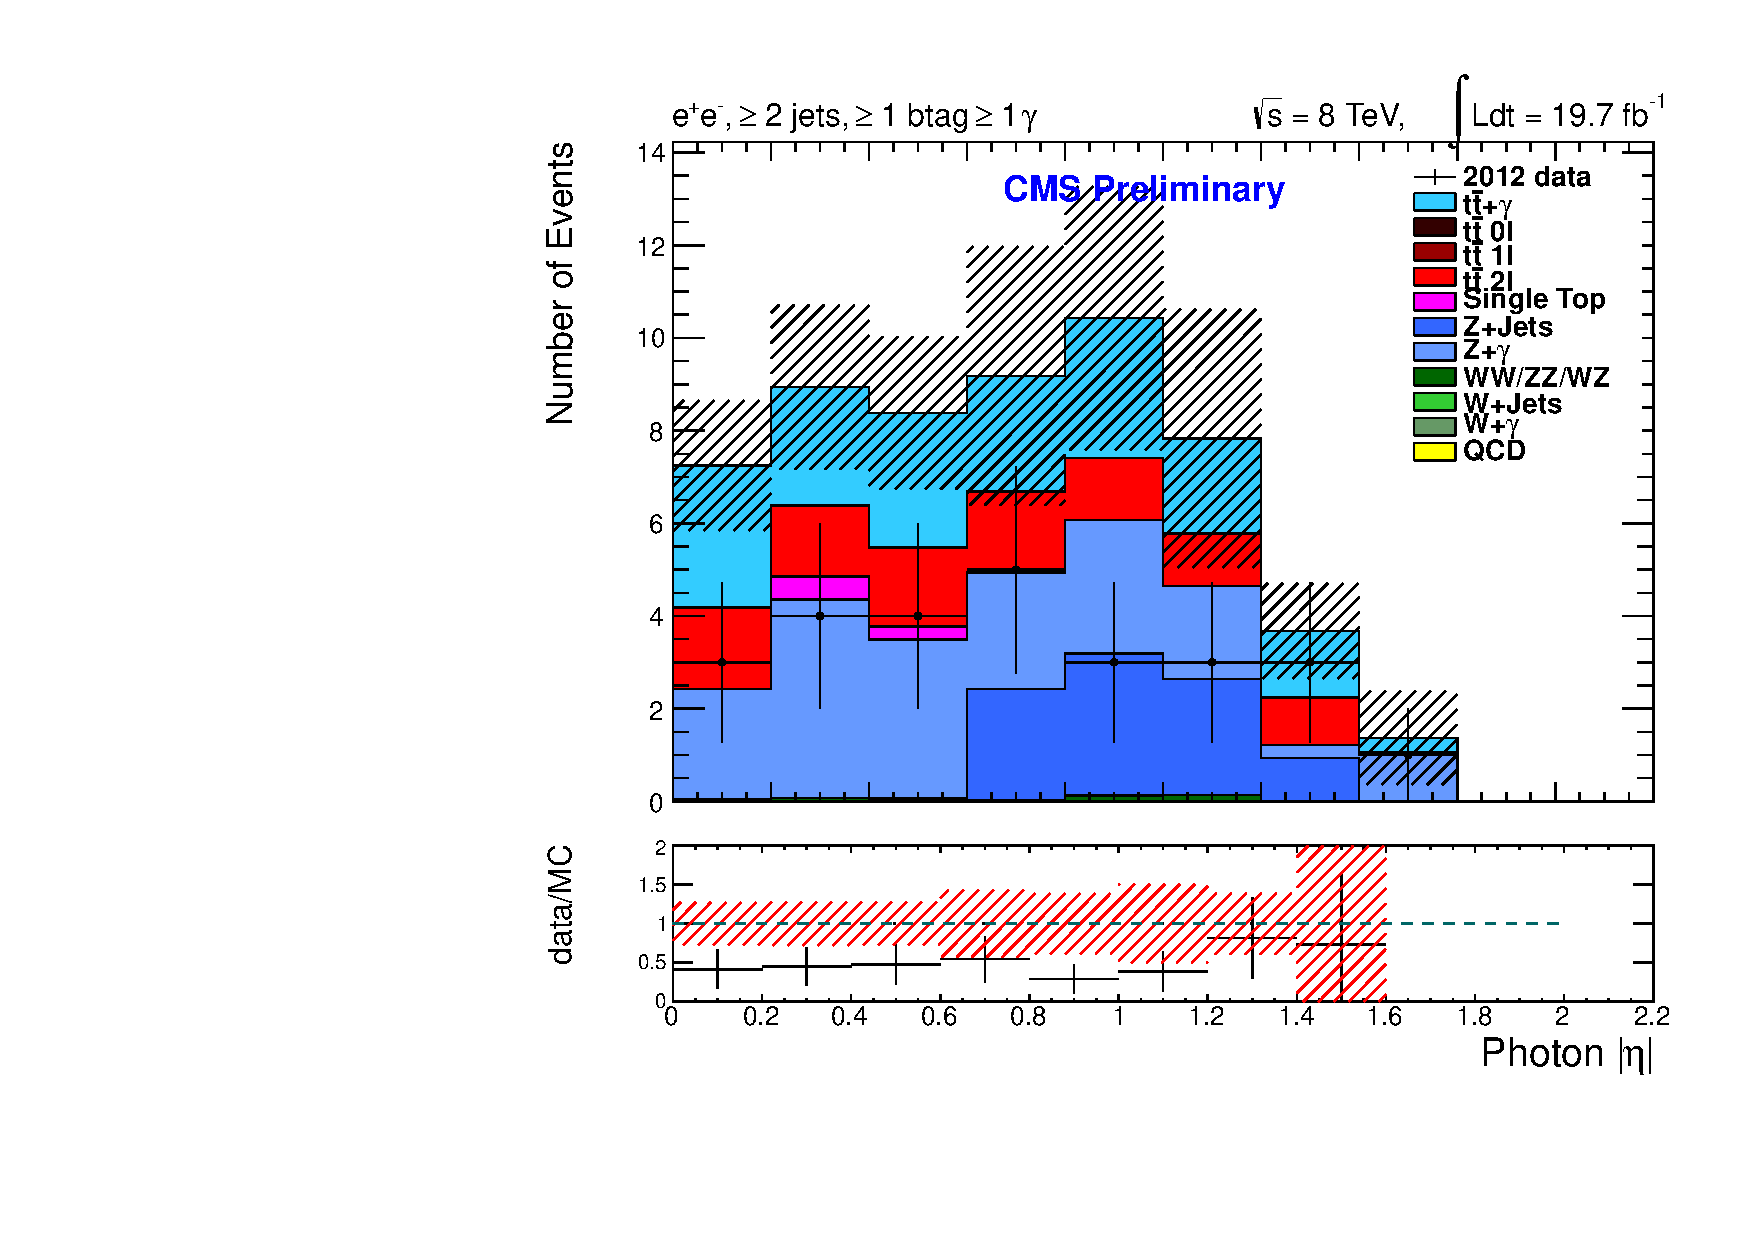
\includegraphics[width=0.5\textwidth]{Plots/ControlPlots/TTbarPhotonAnalysis/EE/Photons/SignalPhotons/Photon_AbsEta_splitTTbar_ratio.pdf} \\
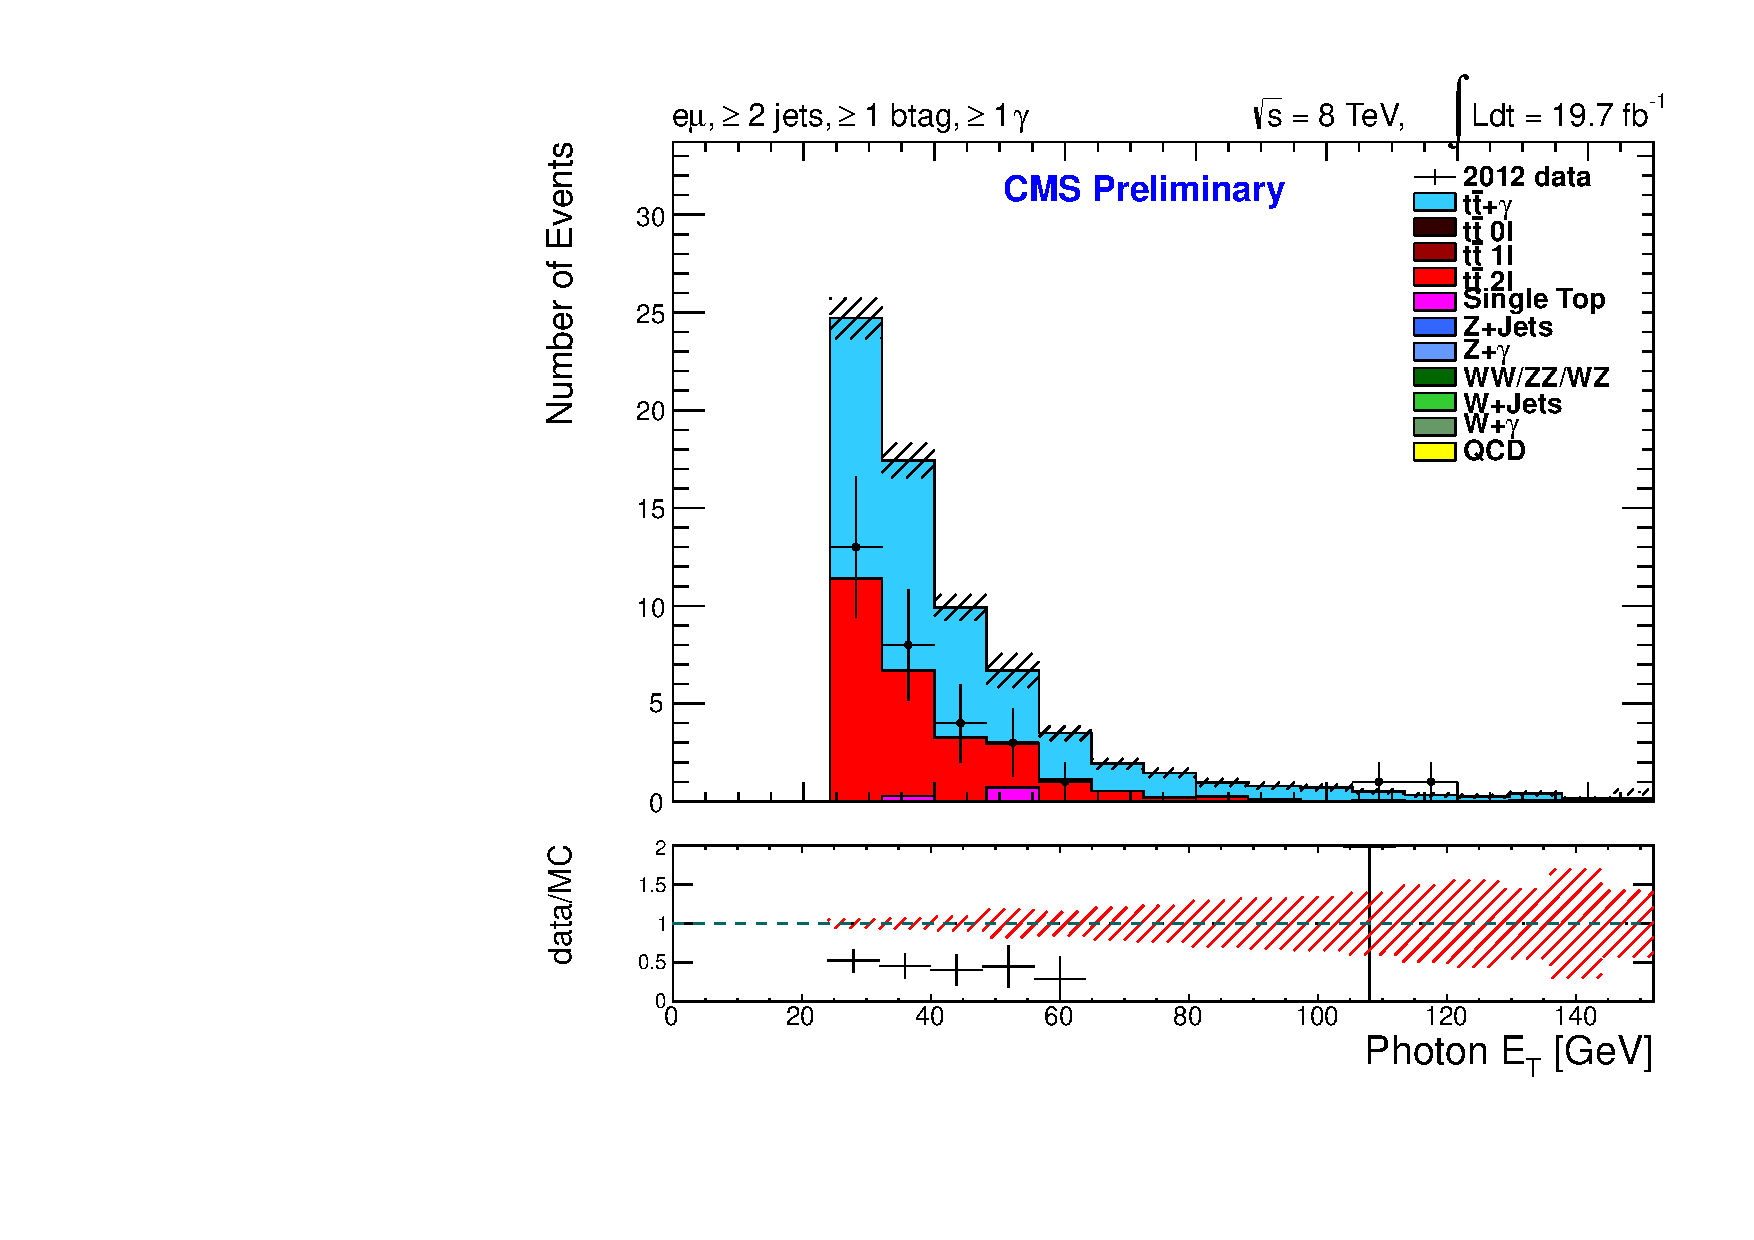
\includegraphics[width=0.5\textwidth]{Plots/ControlPlots/TTbarPhotonAnalysis/EMu/Photons/SignalPhotons/Photon_ET_splitTTbar_ratio.pdf}
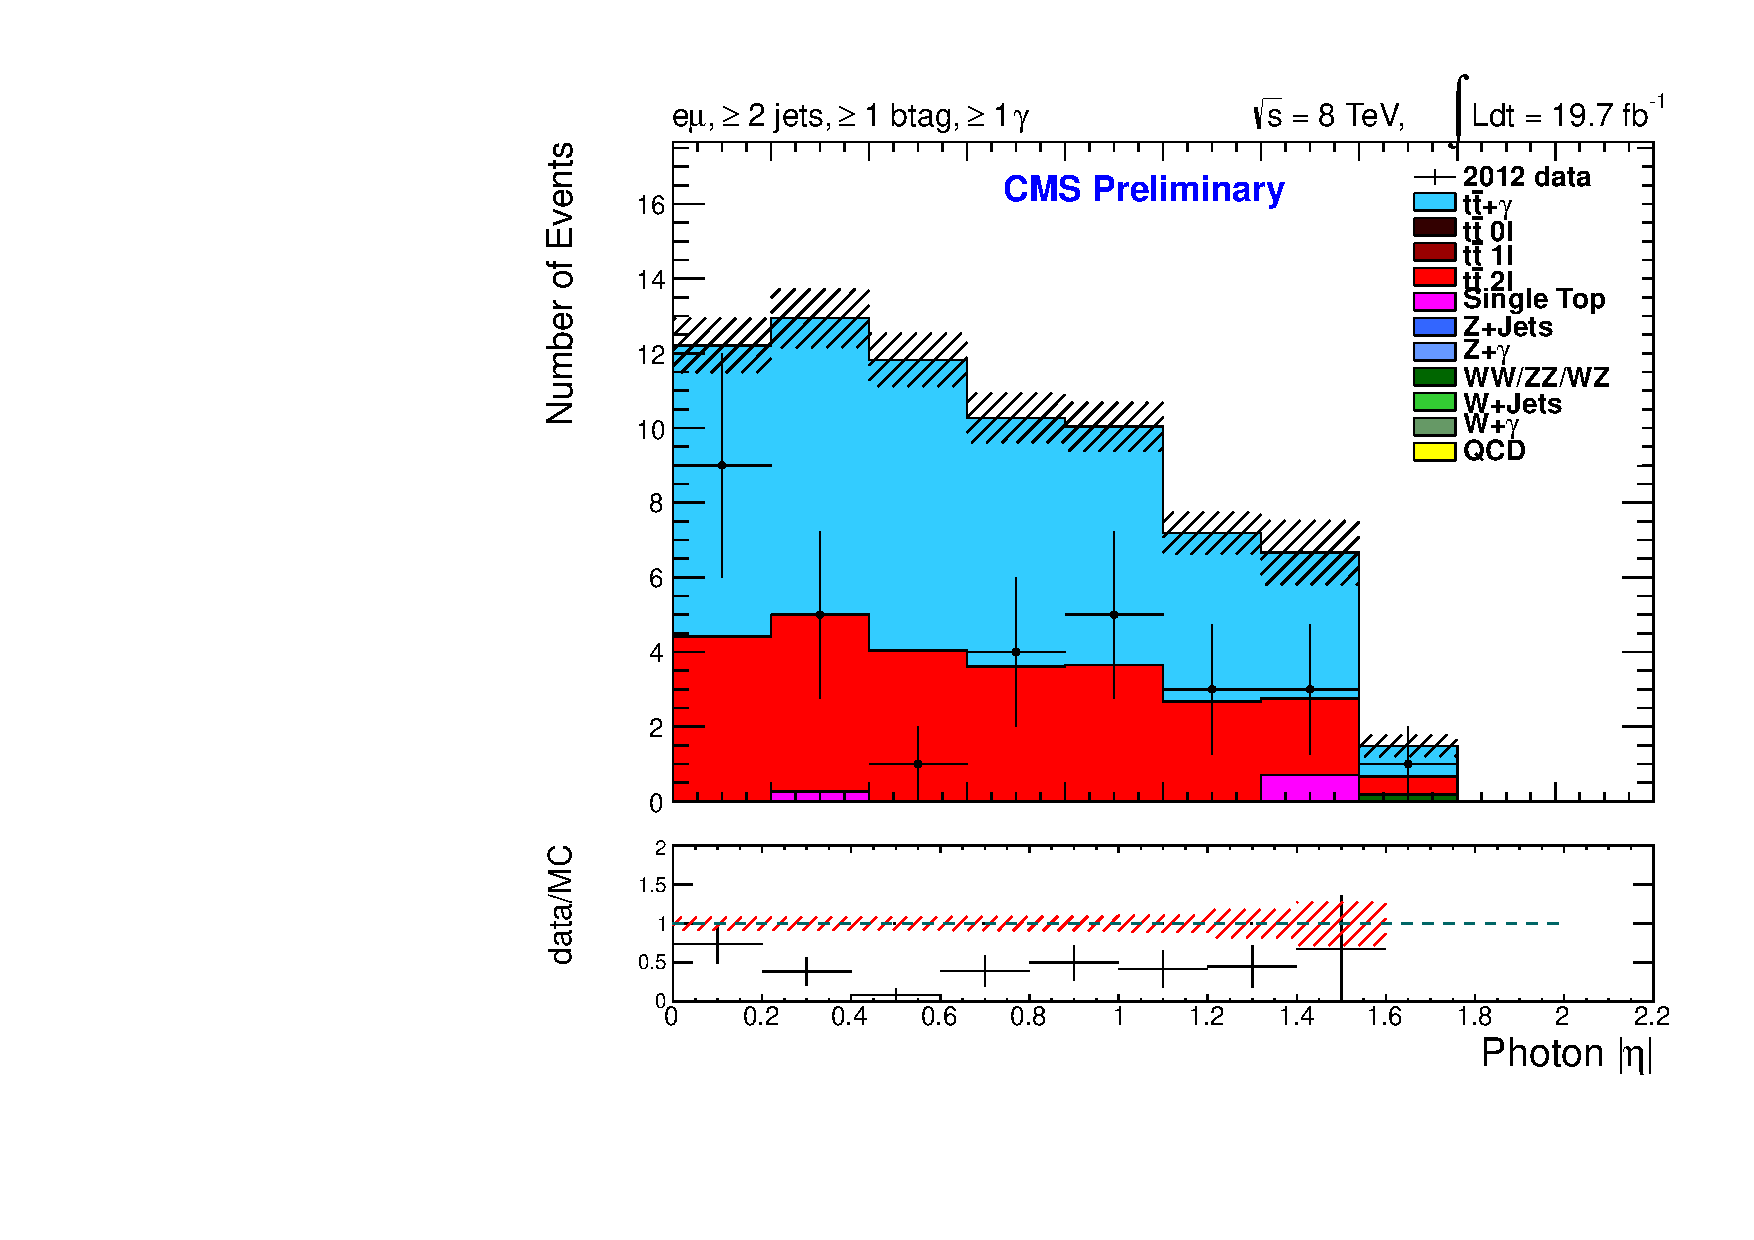
\includegraphics[width=0.5\textwidth]{Plots/ControlPlots/TTbarPhotonAnalysis/EMu/Photons/SignalPhotons/Photon_AbsEta_splitTTbar_ratio.pdf} 
% \end{center}
\caption{Comparison of photon E$_{T}$ and $|\eta|$ distributions in data and simulation in the $\mu^{+}\mu^{-}$, $e^{+}e^{-}$, and $e\mu$ channels after photon selection.}
\label{fig-photonSelectionETandEta}
\end{figure}

\subsection{Cut based photon ID}

The cut-based photon isolation cuts are taken from the recommended values \cite{CutBasedIsolation2012}, with the inclusion of supercluster footprint-removed isolation (see Section \ref{subsec-SCFR}), and are descirbed below.

\begin{description}

\item[Electron Conversion Veto] A boolean to help distinguish an electron from a photon. We should not see a track seed in the pixel detector when identifying a photon. 

\item[Tower Based H/E] The ratio of energy deposited in the Hadronic Calorimeter (HCAL) divided by the fraction of energy deposited in the Electromagnetic Calorimeter (ECAL). This cut is introduced with the requirement that the energy ratio should be less than 5\%.

\item[Shower Width $\sigma_{i\eta i\eta}$] The shower shape weighted by energy, defined as: 

\begin{equation}
\sigma_{i\eta i\eta} = \left(\frac{\sum(\eta_i - \bar{\eta})\omega_i}{\sum\omega_i}\right)^{1/2};  \bar{\eta} = \frac{\sum\eta_i\omega}{\sum\omega_i};  \omega_i = \text{max}\left(0, 4.7 +
\text{log}\frac{E_i}{E_{5x5}}\right).
\end{equation}

This is a key variable in this analysis and will be discussed in greater detail in Section \ref{sec-BackgroundEstimation}.

\item[Charged Hadron Isolation] The isolation of charged hadrons with energy density correction, $\rho$, applied. Cut given as $I_{Char.had} < 1.5 + 0.04*E_T(\gamma)$ GeV. 

\item[Neutral Hadron Isolation] The isolation of neutral hadrons with energy density correction , $\rho$, applied. Cut given as $I_{Neut.had} < 1.0 + 0.005*E_T(\gamma)$ GeV. 

\item[Photon Isolation] The isolation of the photon $I_{\gamma}$, with energy density correction applied. Cut given as $I_{\gamma} < 1.0 + 0.005*E_T(\gamma)$ GeV.


\item[Supercluster footprint-removed Charged Hadron Isolation] The super-cluster footprint-removed isolation of charged hadrons with energy density correction, $\rho$, applied.
Cut given as $I_{char.had} < 5 \ \text{GeV} $. 

\item[Supercluster footprint-removed Neutral Hadron Isolation] The super-cluster footprint-removed isolation of neutral hadrons with energy density correction , $\rho$, applied.
Cut given as $I_{neut.had} < 1.0 + 0.005*E_T(\gamma)$ GeV. 

\item[Supercluster footprint-removed Photon Isolation] The super-cluster footprint-removed isolation of the photon $I_{\gamma}$, with energy density correction applied. Cut given
as $I_{\gamma} < 1.0 + 0.005*E_T(\gamma)$ GeV. 

\end{description}

It must be noted that only supercluster footprint-removed charged hadron isolation is used in this analysis, where PF isolation is used for neutral hadron and photon isolation as described above. 

\subsection{Final state radiation suppression}

It is crucial that initial and final state radiation (ISR/FSR) is modelled correctly for this analysis as photons from initial and final state radiation are not considered as signal and we therefore implement cuts in $\eta$ and $\phi$ to reduce these events. The definition of isolation has been modified from the recommended values in order to make the data-driven estimate of the selection purity more robust.

\begin{description}
\item[$\Delta R(\gamma, leptons)$] In order to diminish FSR in final state leptons, e.g photons radiated off high $p_T$ muons, a minimum distance criterion in the $\eta - \phi$ plane is implemented. The cut is given as $\Delta R(\gamma, leptons) > 0.3$.

\item[$\Delta R(\gamma, jets)$] In order to reduce FSR in final state partons a minimum distance criterion in the $\eta - \phi$ plane is implemented. The cut is given as $\Delta R(\gamma, jets) > 0.3$.

\item[$\Delta R(leptons, jets)$] In order to reduce FSR in final state partons a minimum distance criterion in the $\eta - \phi$ plane is implemented. The cut is given as $\Delta R(leptons, jets) > 0.3$.
\end{description}

A significance test was performed in an attempt to optimise the $\Delta R$ cut between final state leptons and jets, however this proved inconclusive due to an initial cut of $\Delta R > 0.1$ at generator level. Figure \ref{fig-photonDRjets} shows the $\Delta R$ distributions after photon selection.

\begin{figure}
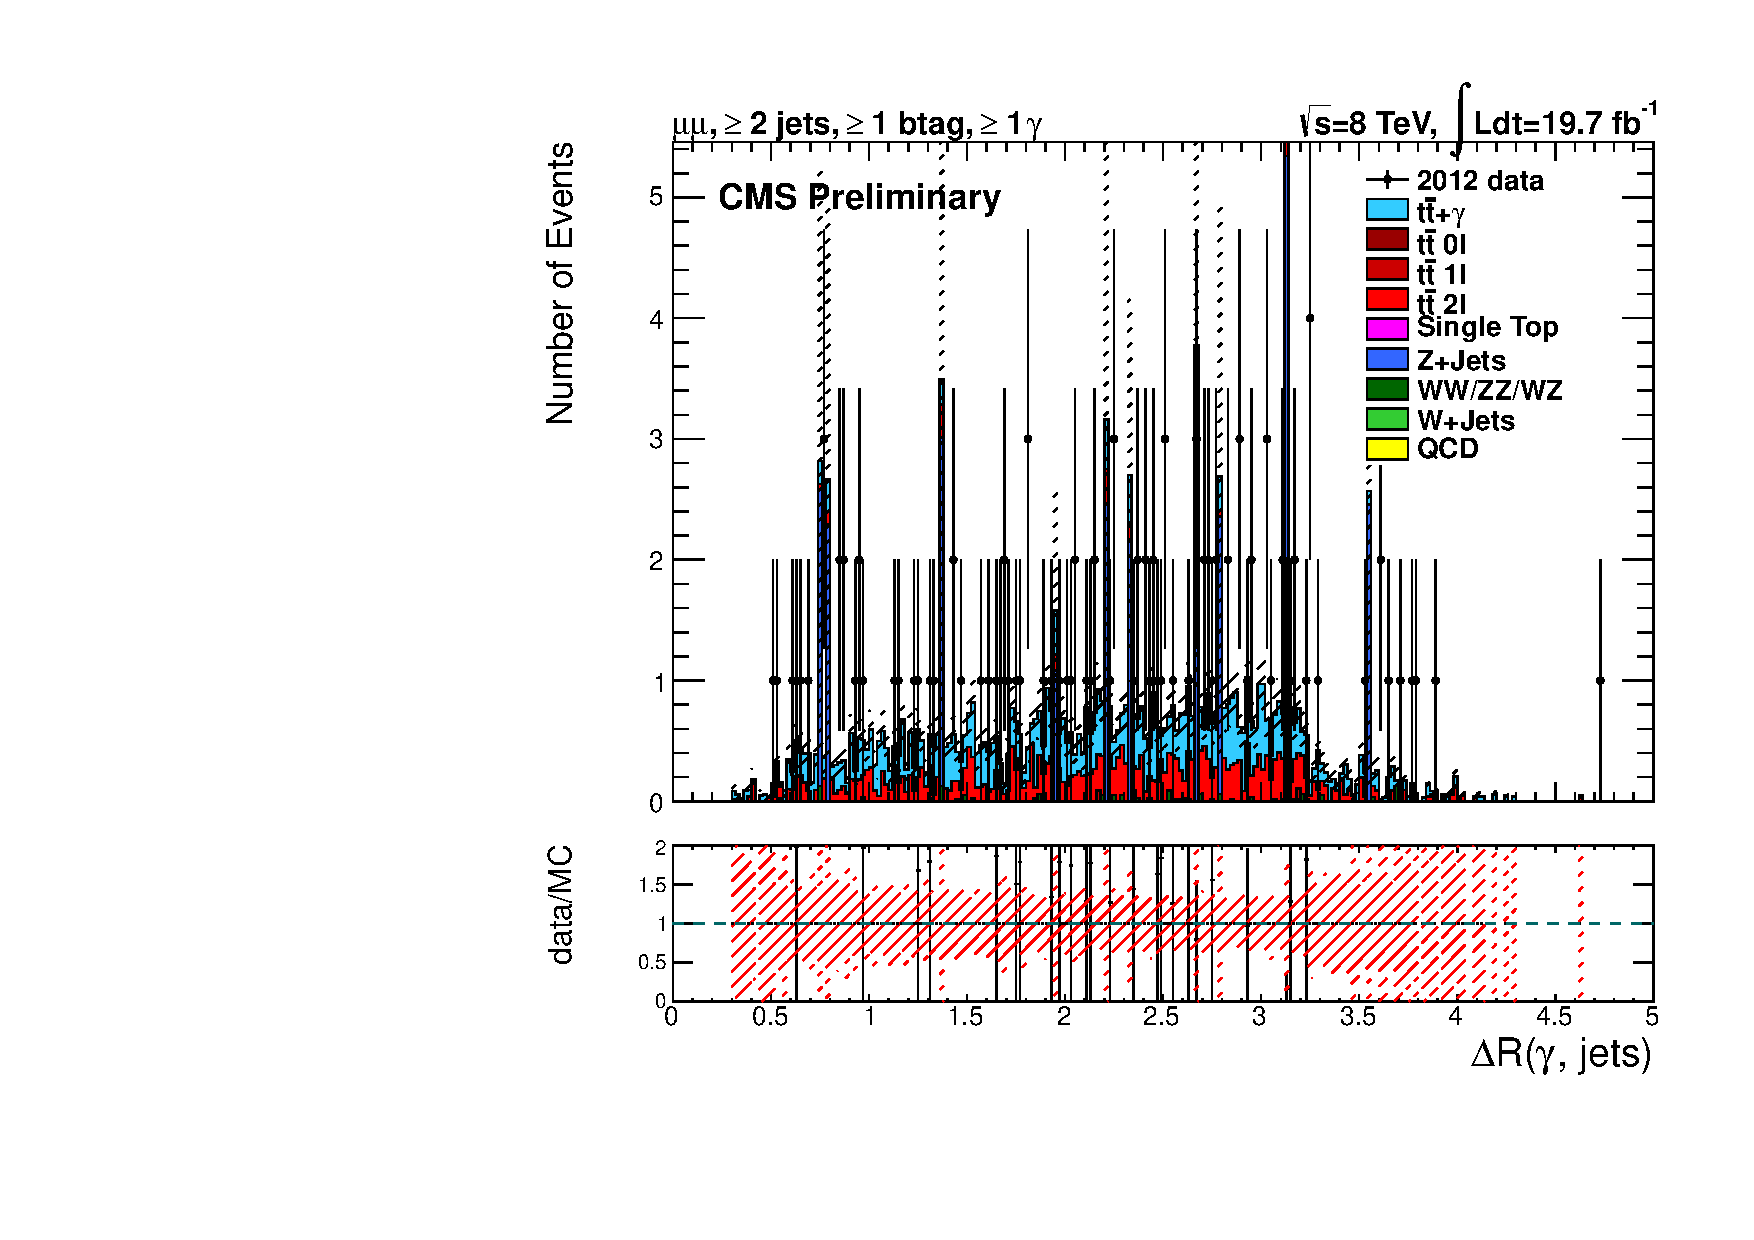
\includegraphics[width=0.5\textwidth]{Plots/ControlPlots/TTbarPhotonAnalysis/MuMu/Photons/SignalPhotons/Photon_deltaR_jets_splitTTbar_ratio.pdf}
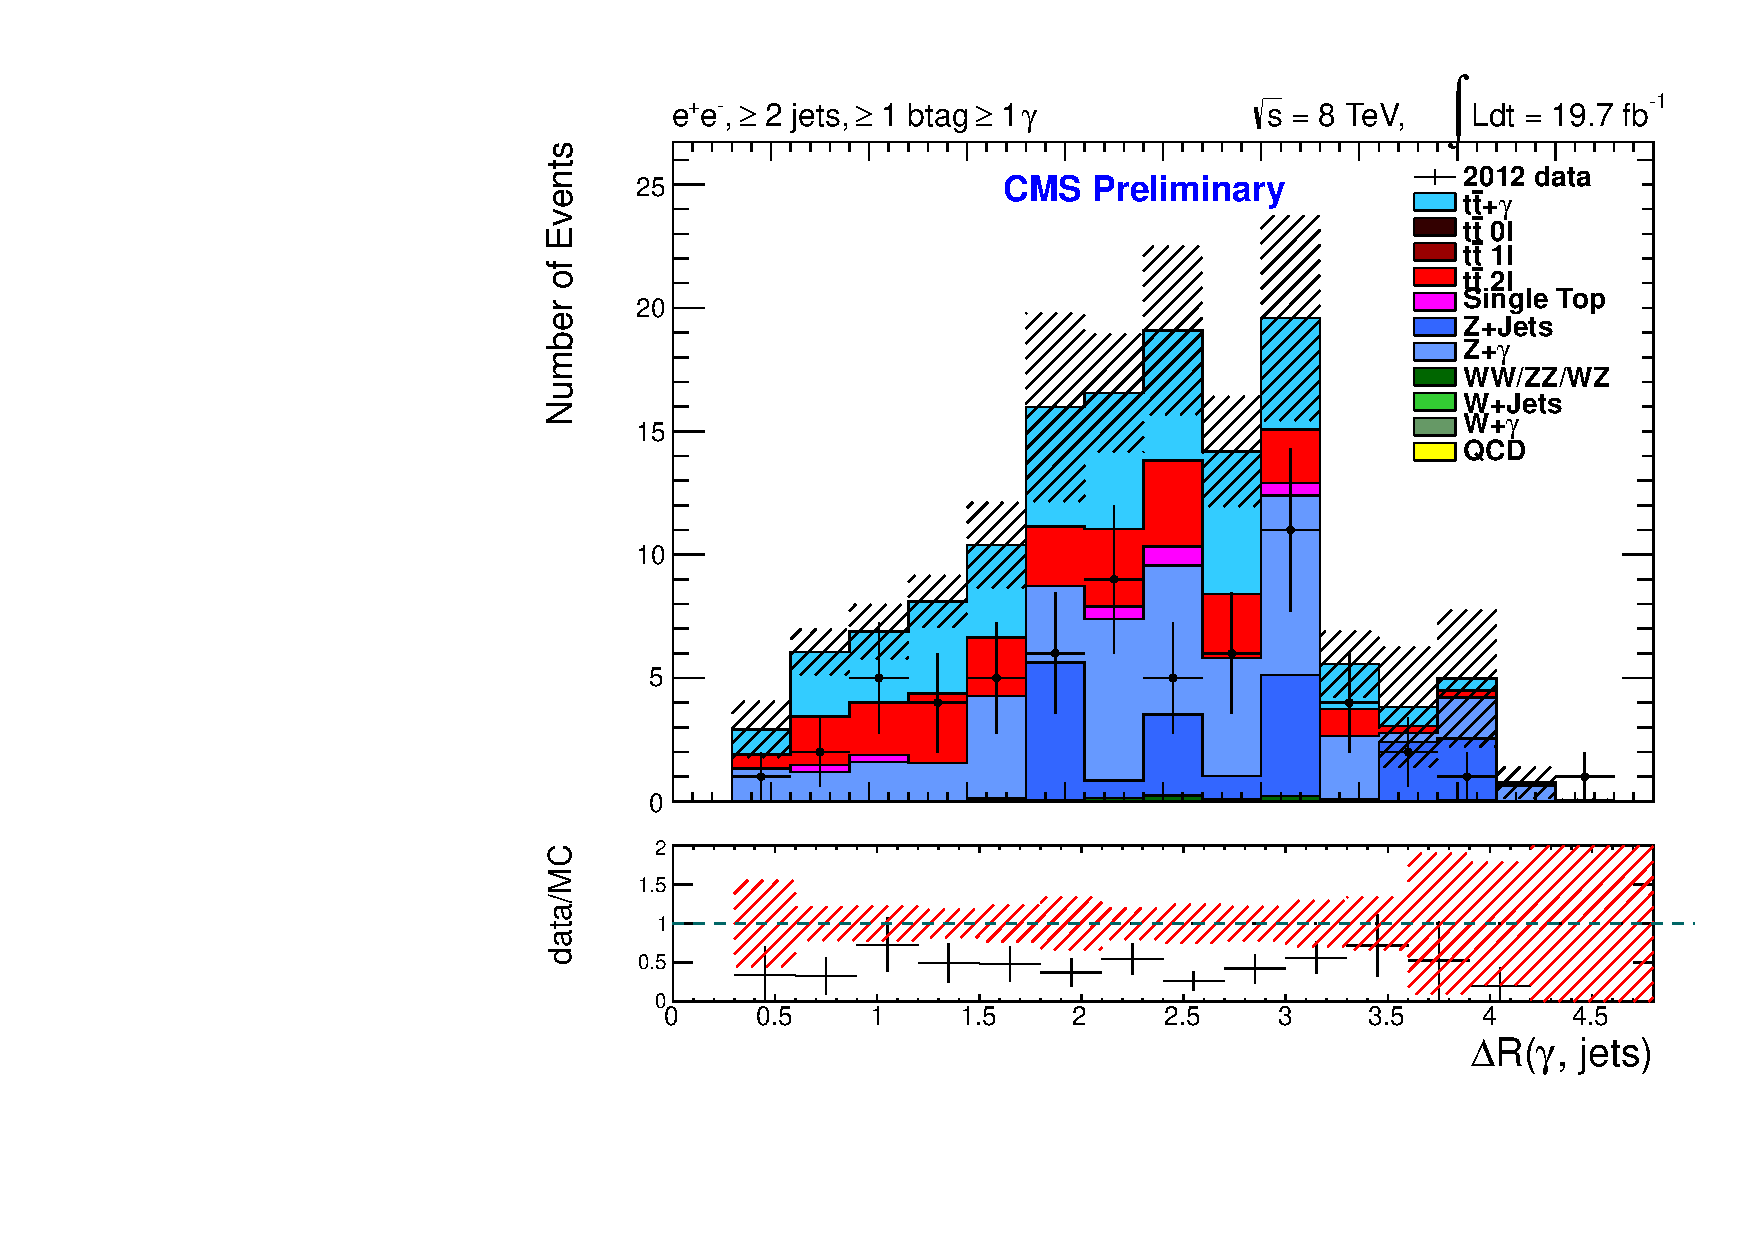
\includegraphics[width=0.5\textwidth]{Plots/ControlPlots/TTbarPhotonAnalysis/EE/Photons/SignalPhotons/Photon_deltaR_jets_splitTTbar_ratio.pdf}\\
\begin{center}
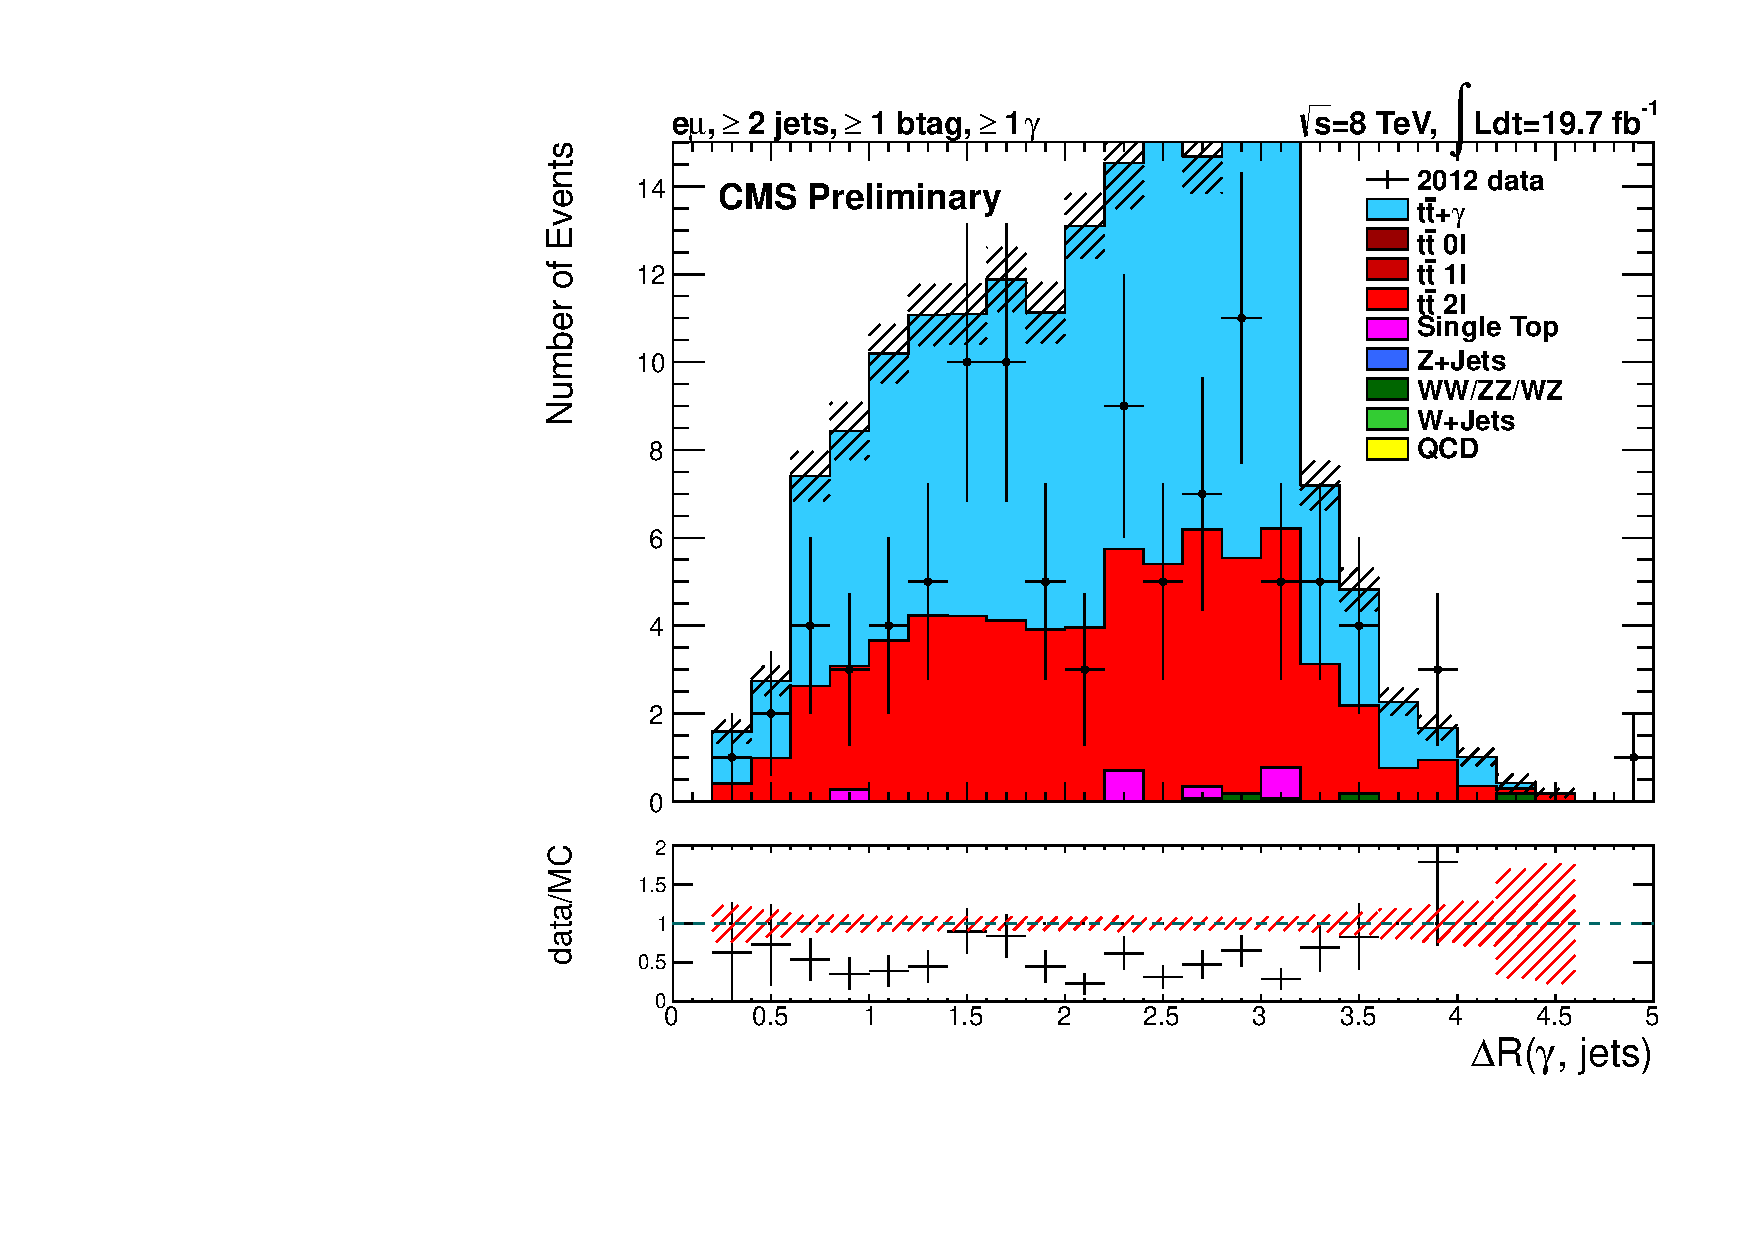
\includegraphics[width=0.5\textwidth]{Plots/ControlPlots/TTbarPhotonAnalysis/EMu/Photons/SignalPhotons/Photon_deltaR_jets_splitTTbar_ratio.pdf}
\end{center}
\caption{Comparison of the $\Delta R(\gamma, jets)$ distributions in data and simulation in the $\mu^{+}\mu^{-}$, $e^{+}e^{-}$, and $e\mu$ channels after photon selection.}
\label{fig-photonDRjets}
\end{figure}

The distributions for the other photon variables can be seen in Figure \ref{fig-photonPlots}

\subsection{Super-cluster footprint-removal for photon isolation} \label{subsec-SCFR}

The $t\bar{t}+\gamma$ analysis uses a method of removing the photon shower energy deposit, or ``footprint", from the isolation cone in order to remove the energy deposits of the selected photon from the isolation sum, and thus minimise correlation the between shower shape and isolation components in our signal process --- super-cluster footprint removal (SCFR). With this method the footprint is, effectively, cleaned so that the isolation sum is not biased from the presence of the photon at the centre of the cone. Shower-shape variables, defined within the super-cluster, are then decoupled from the isolation computation, defined outside of the super-cluster. When the footprint of the photon has finally been removed, the isolation sum for prompt photons is due only to pileup and underlying events. The process calculates each isolation component individually, however we only consider the charged hadron component of the isolation sum using this technique, which is then used to model our background and signal processes. This method was first implemented as a technique upon measuring the diphoton cross-section with 7 TeV data \cite{diffxsectdiphoton}. The main features of this module are improvement in the agreement between data and MC for ECAL detector-based isolation, better discriminating power against the misidentification of photons, and it allows us to use a fully data-driven method for constructing our template fit.

We define photon isolation as the sum of the transverse momenta of all particles falling within the isolation cone surrounding the photon candidate. We define the isolation cone to be within a $\Delta R < 0.3$, where $\Delta R = \sqrt{(\Delta\eta)^2+(\Delta\phi)^2}$. The momentum of the prompt photon should not contribute to the isolation sum, and thus particles found close to the photon footprint are not included within the sum. 

SCFR is a purely geometrical procedure which is computed as follows:

\begin{description}
	\item[Step 1]: Propagate the PF candidate trajectory from the primary vertex to the surface of the ECAL. We must take into account the magnetic field for charged hadron candidates. The impact parameter, $d_z$, is calculated in the z direction with respect to the primary vertex, neglecting the transverse distance, $d_{xy}$. 
	\item[Step 2]: If the propagated PF candidate is found to hit the surface of a crystal lying within the super-cluster, then the candidate is therefore removed from the isolation sum, as shown in Figure \ref{fig-SCFR}. The PF candidate is allowed to fall within a volume of 25\% of the crystal size around the crystal, in order to account for the fact that the PF candidate's energy deposit has a finite extension in the ECAL, and thus has a reasonably large effect at the edges of the super-cluster. 
\end{description}

This is such that the super-cluster shape defines the region which is excluded from the isolation cone in each event.

In the standard particle flow algorithm isolation is calculated on an individual basis for PF candidates divided into three groups: Charged hadrons, neutral hadrons, and photons. This procedure carries potential pit-falls, listed below.

\begin{itemize}
	\item When computing the sum of isolation, any energy deposit that is not associated with a reconstructed particle is not included within the sum.  
	\item When reconstructing a photon, its energy may be dispersed over a large radius within the detector, and thus reconstructed as several particles. This will greatly affect the isolation of the photon.
\end{itemize}

This does not have too much of an impact when using the standard cut-based particle IDs, such as used in this analysis, however as we are interested in the isolation profile shape some improvements can be made. 

Super-cluster footprint-removed isolation deals with PF candidates, whereas PF isolation deals with identified particles. This reduces the probability for the first pit-fall to happen. The second pit-fall arises due to the leakage of energy from the photon into the isolation cone around the super-cluster. Therefore, a different method for defining the isolation cone is implemented to overcome this problem, whereby summing the transverse momentum of particle flow candidates that fall within the isolation cone, but which are not close to the super-cluster in the ECAL. The $\eta$ and $\phi$ coordinates of the super-cluster are calculated by checking the position of hits recorded, and if a PF candidate that has been propagated to the surface of the calorimeter lies within the super-cluster, enlarged by 25\%, then the photon is not considered isolation and thus the candidate is not added to the isolation sum. The standard CMS implementation for energy density correction, $\rho$, is applied to the isolation to account for pileup. 

\begin{figure} 
\begin{center}
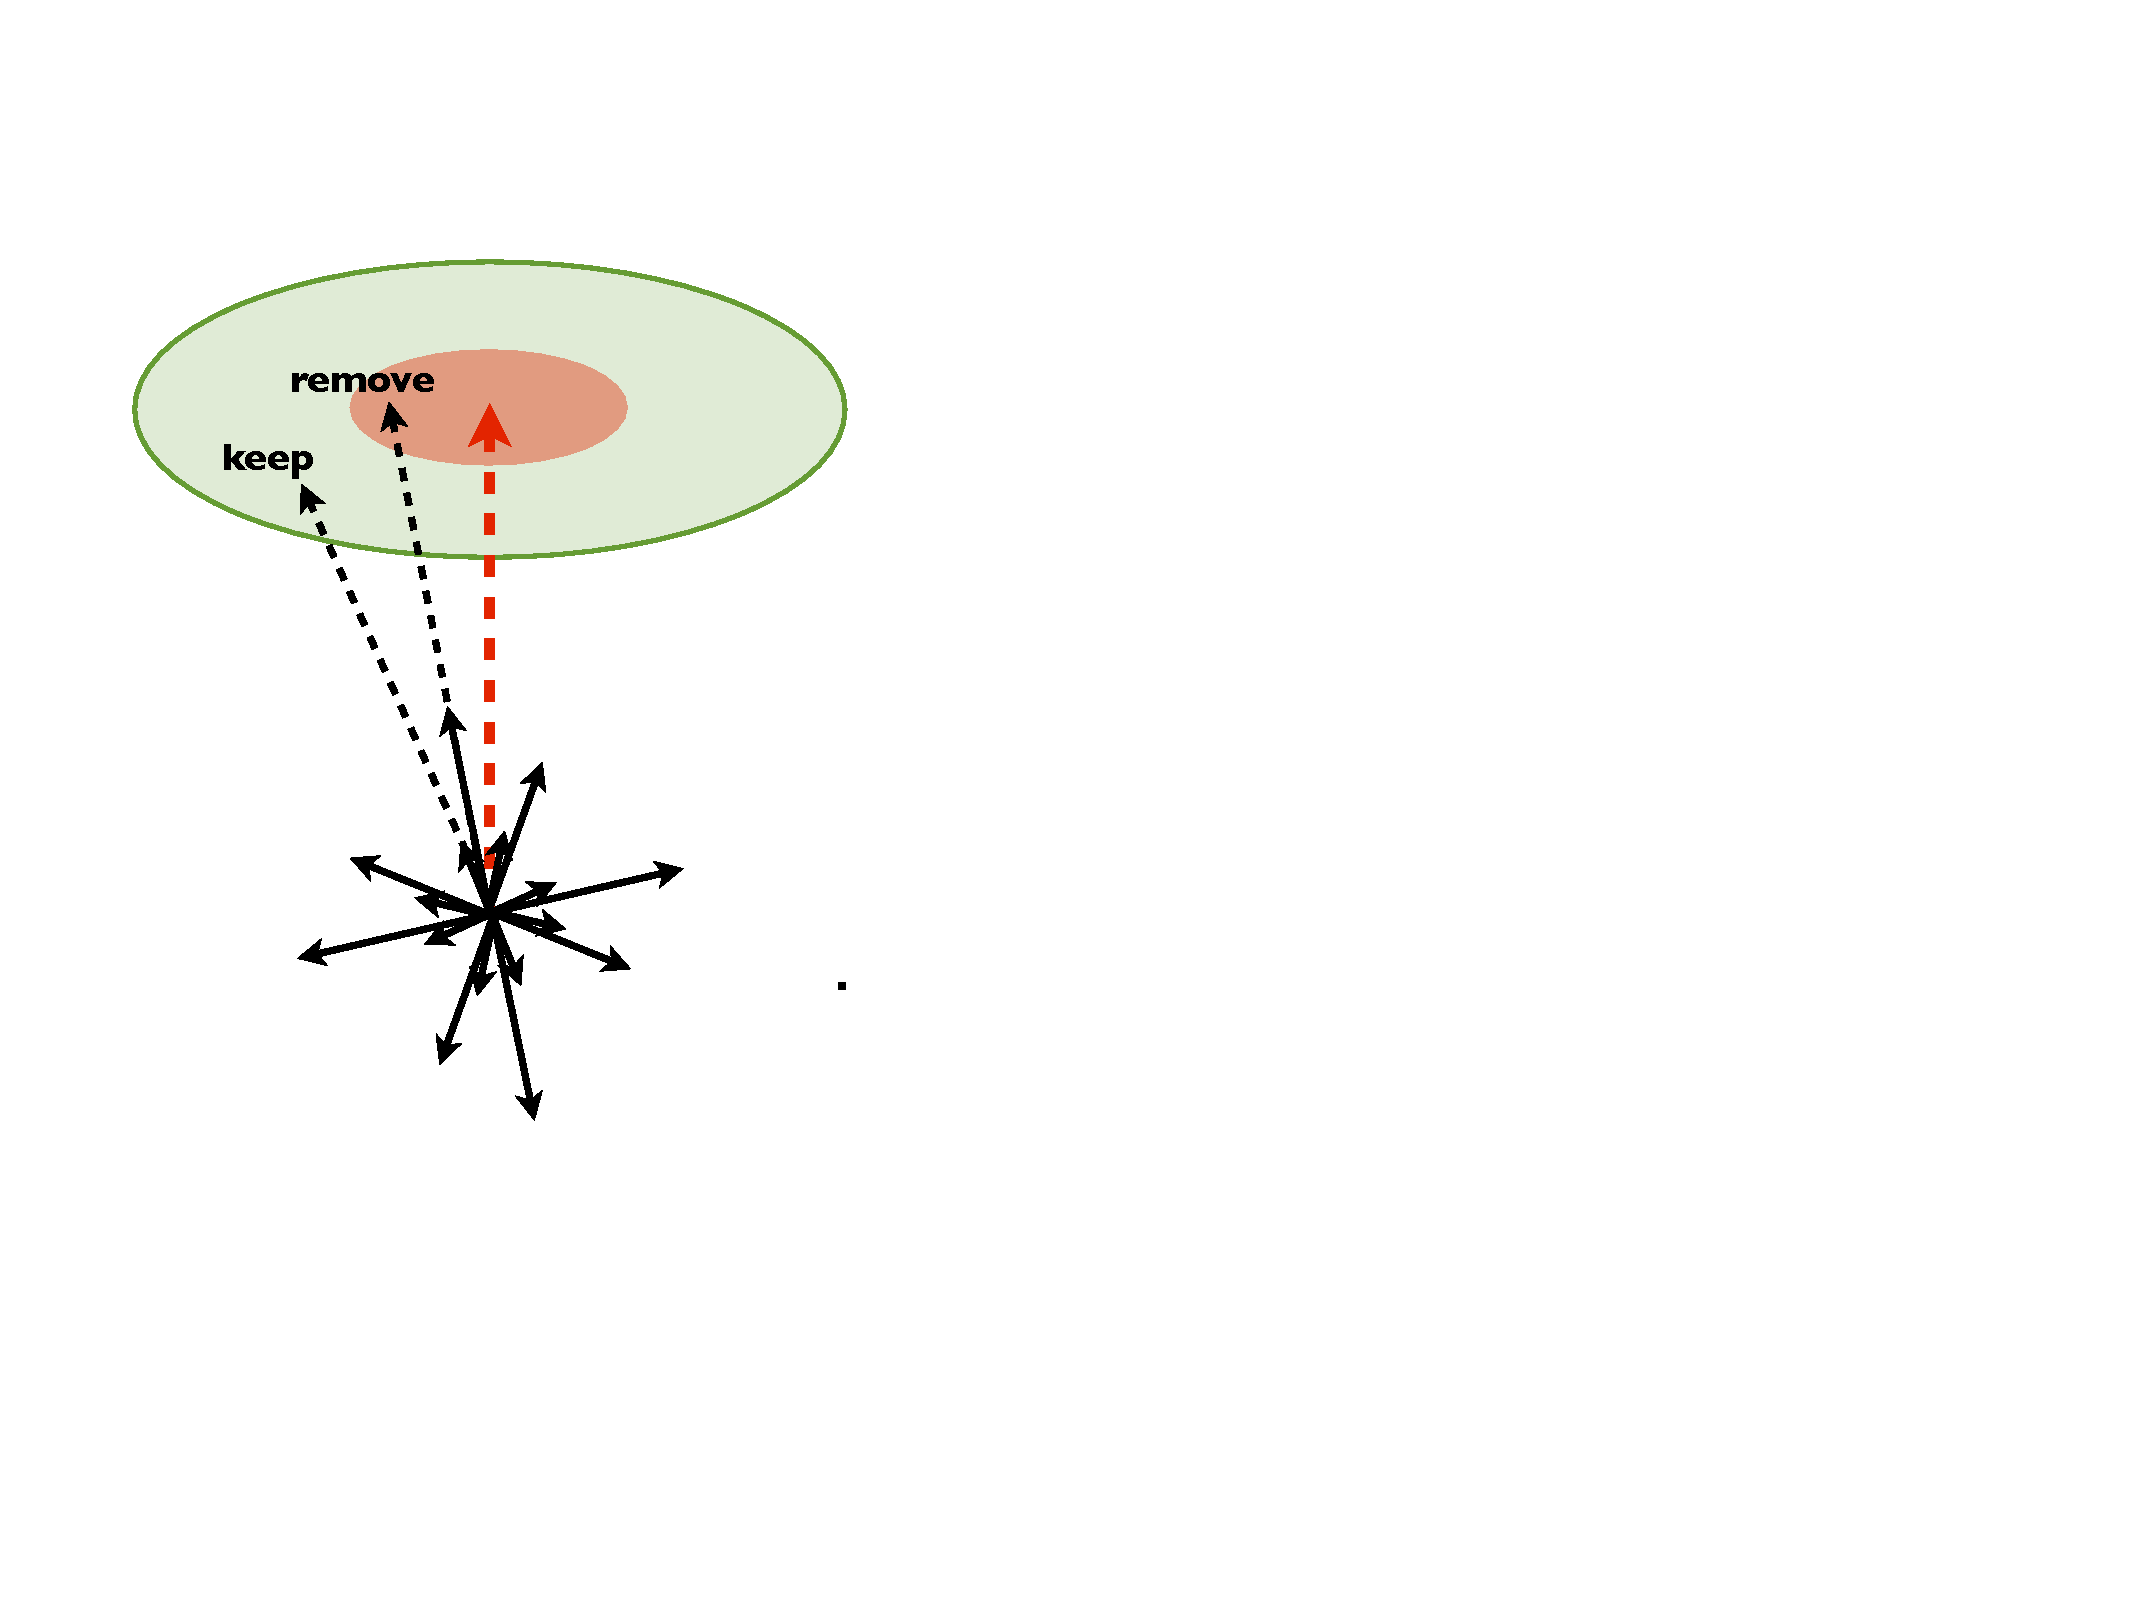
\includegraphics[width=0.4\textwidth]{Figures/RandomCone3.pdf}
\end{center}
\caption{Graphic representation of the PF candidate footprint (in red) from the primary interaction vertex, within the isolation cone (green). \cite{MarcoThesis}}
\label{fig-SCFR}
\end{figure}

\subsection{Signal template construction using the random cone method}

We construct our prompt signal photon template using the ``random cone" method. The events that pass our full photon event selection are used as the method relies on the assumption that a prompt photon is isolated, such that the activity recorded within the detector around the prompt photon, not regarding the area affected by the energy deposit from the photon, arises only from pile-up, underlying events, and electronic noise in the ECAL.  

Contributions from these effects, generally, do not vary for an isolation sum which is calculated in a region which is separate from the photon candidate, but using the same pseudorapidity range, $\phi$. A suitable orientation of the isolation cone is chosen by using the proceeding steps:

\begin{itemize}
	\item We define a direction which is obtained from the photon candidate direction, and then rotating by a random angle, $\phi_{Rand.Cone}$ between $0.8$ and $2\pi - 0.8$ radians, around the z-axis of the detector system (or rotating in $\phi$ with a fixed $\eta$) as shown in Figure \ref{fig-RandomConeIsolation}. This is designed such that an isolation cone with $\Delta R = 0.4$ centred on the random cone axis would not overlap with an isolation cone which is centred on the photon candidate, or an object that is produced back-to-back with respect to it.
	\item We then check for objects lying within the region, such that there is no energy originating from anything other than pile-up, underlying events, or electrical noise in the ECAL. Such that there are no AK5\footnote{Anti-$k_T$ jet clustering algorithm with cone size of $\Delta R = 0.5$ (see Section \ref{subsec-JetReconstruction})} PF jets with a p$_T$ of at least 20 GeV at $\Delta R < 0.8$, photons with p$_T$ less than 10 GeV at $\Delta R < 0.8$, or muons at $\Delta R < 0.4$ with respect to the random cone axis. If such an object is found to fulfil our requirements, then we perform the same search again to generate another random angle, $\phi_{Rand.Cone}$, until a suitable direction is found. In practice, the procedure is not repeated more than twice in order to find a suitable direction.   
\end{itemize}

We then calculate the isolation sum within a cone centred on our chosen direction. The difference when performing footprint removal now is that there is no super-cluster lying along the cone axis, and therefore it must be performed in a different way: the area corresponding to that in which the photon super-cluster lies, which is rotated in $\phi_{Rand.Cone}$ in order to align with the random cone axis, is not included within the calculation process. In this manner, both the area which we consider for the isolation sum, and the area throughout the centre of the cone replacing the photon candidate footprint, has exactly the same shape and extension in the photon and random cone directions.   

\begin{figure} 
\begin{center}
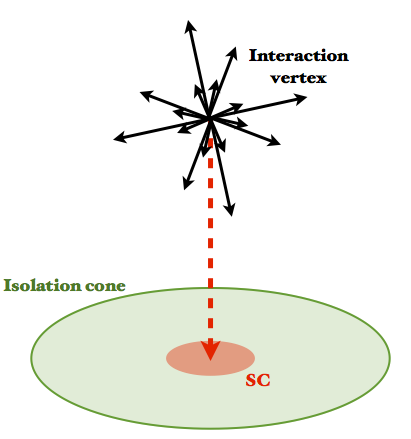
\includegraphics[width=0.45\textwidth]{Figures/RandomCone1.png}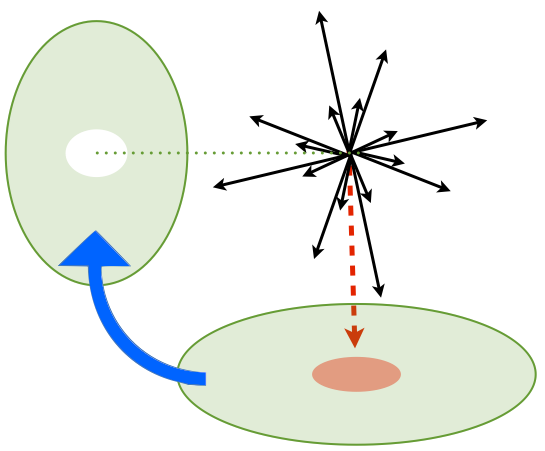
\includegraphics[width=0.55\textwidth]{Figures/RandomCone2.png}
\end{center}
\caption{Illustration of the random cone technique. Under the assumption that the footprint of the photon (red) is completely removed from the isolation sum, the energy deposited in the random-cone area (green in right image) predicts the energy deposited in the isolation cone (green area in left image). \cite{MarcoThesis}}
\label{fig-RandomConeIsolation}
\end{figure}

\section{Background Estimation} \label{sec-BackgroundEstimation}

\subsection{Background estimation using the $\sigma_{i \eta i \eta}$ side-band method} 

Background events are identified as non-prompt or misidentified photons. We define a template to model our background by selecting photon candidates that fail one selection requirement, which we call the ``side-band" region. The logic behind this method is such that by inverting a particular cut on the photon selection, then we have a sample that is rich in ``photon-like" jets (whereby the hadronisation process resolves to a neutral boosted meson with very little activity around it). In order to model the background correctly, we must select the requirements on the side-band region such that they do not differ too greatly from the full selection, and thus we do not incorrectly reject a genuine jet. 

For the $t\bar{t}+\gamma$ analysis, we create a side-band region by inverting the shower-shape selection cut, thus giving a cut of $0.12 < \sigma_{i \eta i \eta} < 0.20$ where all other photon ID selection requirements still remain the same. When considering a side-band variable, we choose a variable with little to no correlation with our template variable in order to optimise the performance of the method. The shape of the side-band template will then closely resemble the isolation distribution for photons that are not prompt but pass the photon ID requirements. 

We calculate the shower shape of the photon by measuring energy deposits from within a $5 \times 5$ matrix of crystals, centred around the crystal with the largest energy in the super-cluster. As the super-cluster footprint-removal technique removes the super-cluster from the isolation sum, then we have no shared input between the two variables (shower shape and isolation) effectively removing any correlation between the two. However, no two variables are ever truly uncorrelated, and any residual correlation can be attributed to the properties of hadronisation of jets. As our main source of fake photons arises in the form of jets misidentified as photons, we use the super-cluster footprint-removed charged hadron isolation as our background template variable to discriminate against the fake photons.

Talk about agreement between data and simulation. 

\begin{figure}
\includegraphics[width=0.5\textwidth]{Plots/signalComparison/MuMu/sigComparison.pdf}
\includegraphics[width=0.5\textwidth]{Plots/signalComparison/EE/sigComparison.pdf}
\begin{center}
\includegraphics[width=0.5\textwidth]{Plots/signalComparison/EMu/sigComparison.pdf}
\end{center}
\caption{Comparison of the shape from random cone isolation and isolated photons identified from generator particle matching in the $\mu^{+}\mu^{-}$, $e^{+}e^{-}$, and $e\mu$ channels.}
\label{fig-signalComparison}
\end{figure}


\begin{figure}
\includegraphics[width=0.5\textwidth]{Plots/signalComparison/MuMu/bkgdComparison.pdf}
\includegraphics[width=0.5\textwidth]{Plots/signalComparison/EE/bkgdComparison.pdf}
\begin{center}
\includegraphics[width=0.5\textwidth]{Plots/signalComparison/EMu/bkgdComparison.pdf}
\end{center}
\caption{Comparison of the isolation profiles from the side band region and isolation of hadronic photons identified from generator particle matching in the $\mu^{+}\mu^{-}$, $e^{+}e^{-}$, and $e\mu$ channels.}
\label{fig-backgroundComparison}
\end{figure}


\begin{figure}
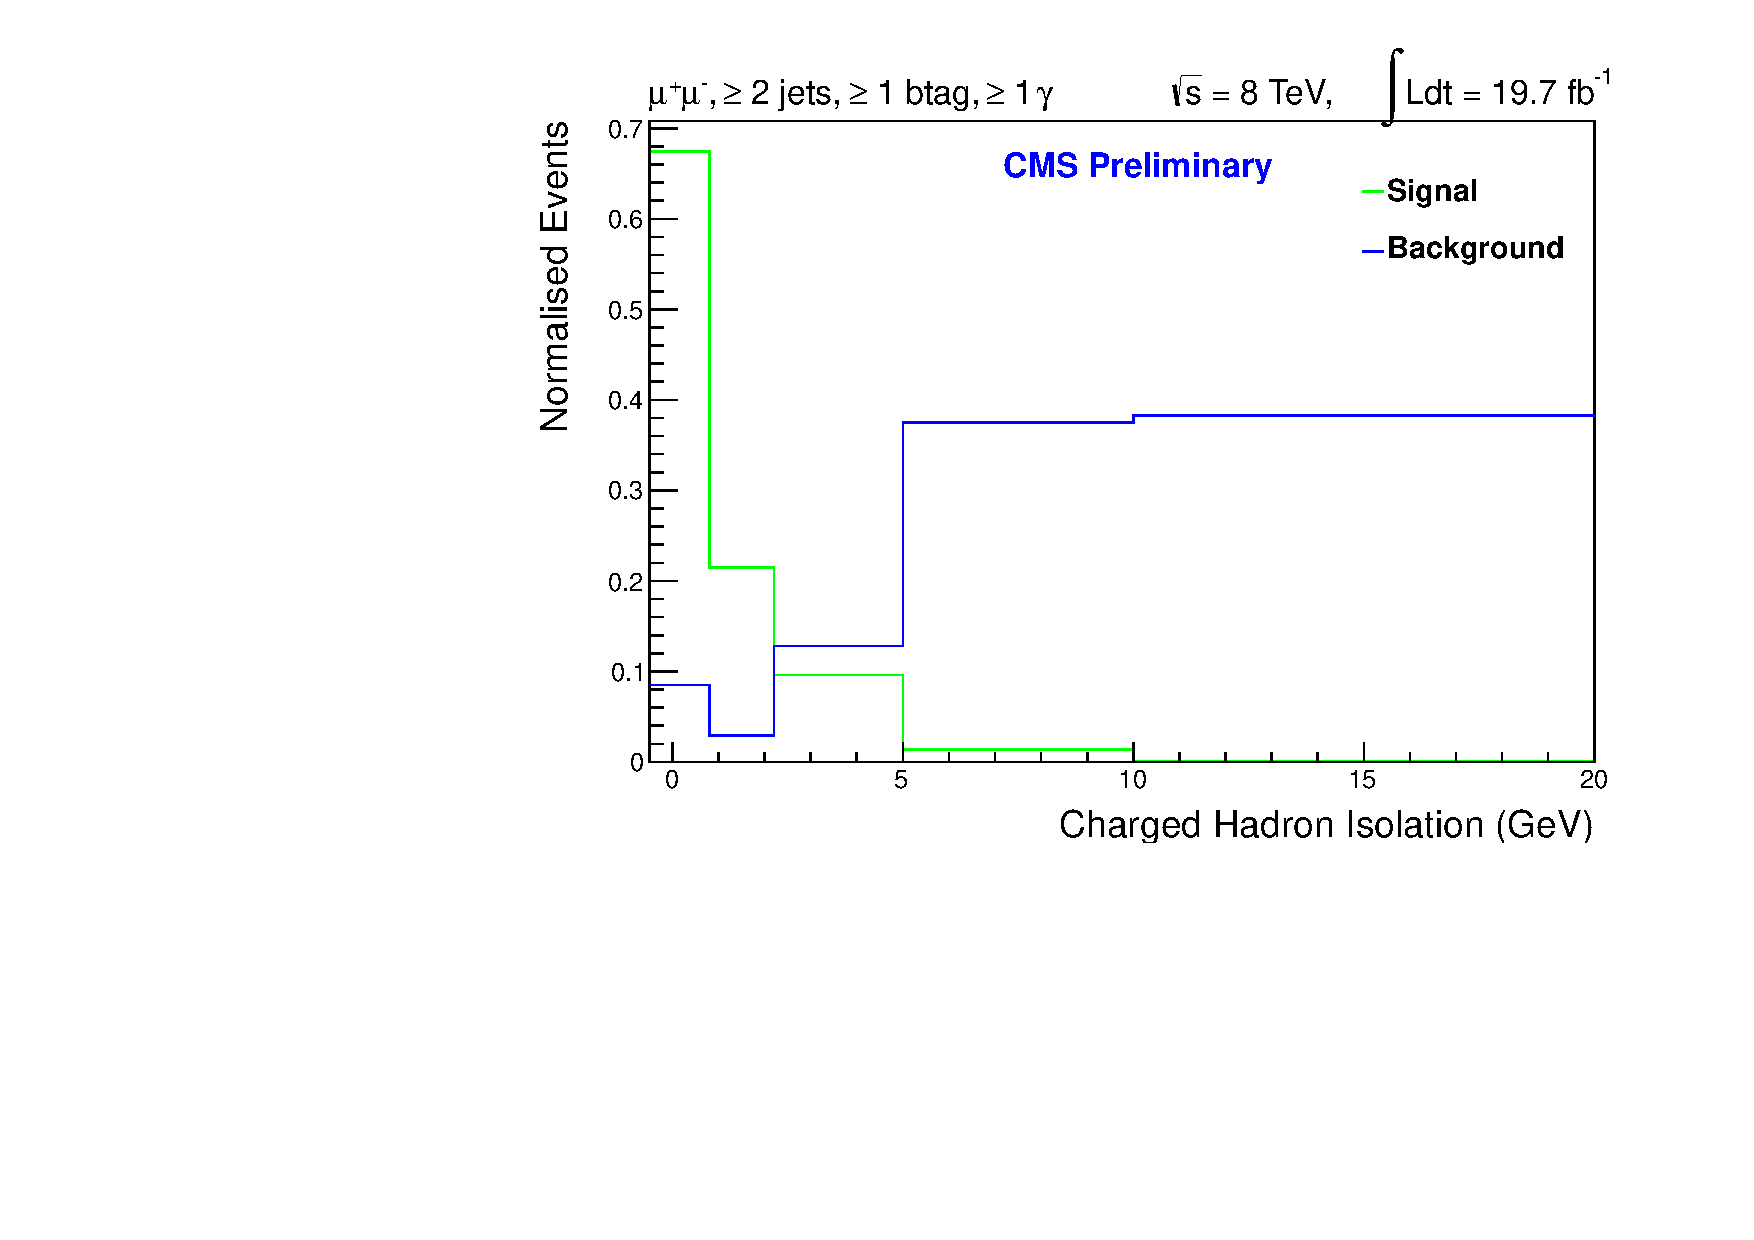
\includegraphics[width=0.5\textwidth]{Plots/Fits/TTbarPhotonAnalysis/MuMu/central/FitTemplate.pdf}
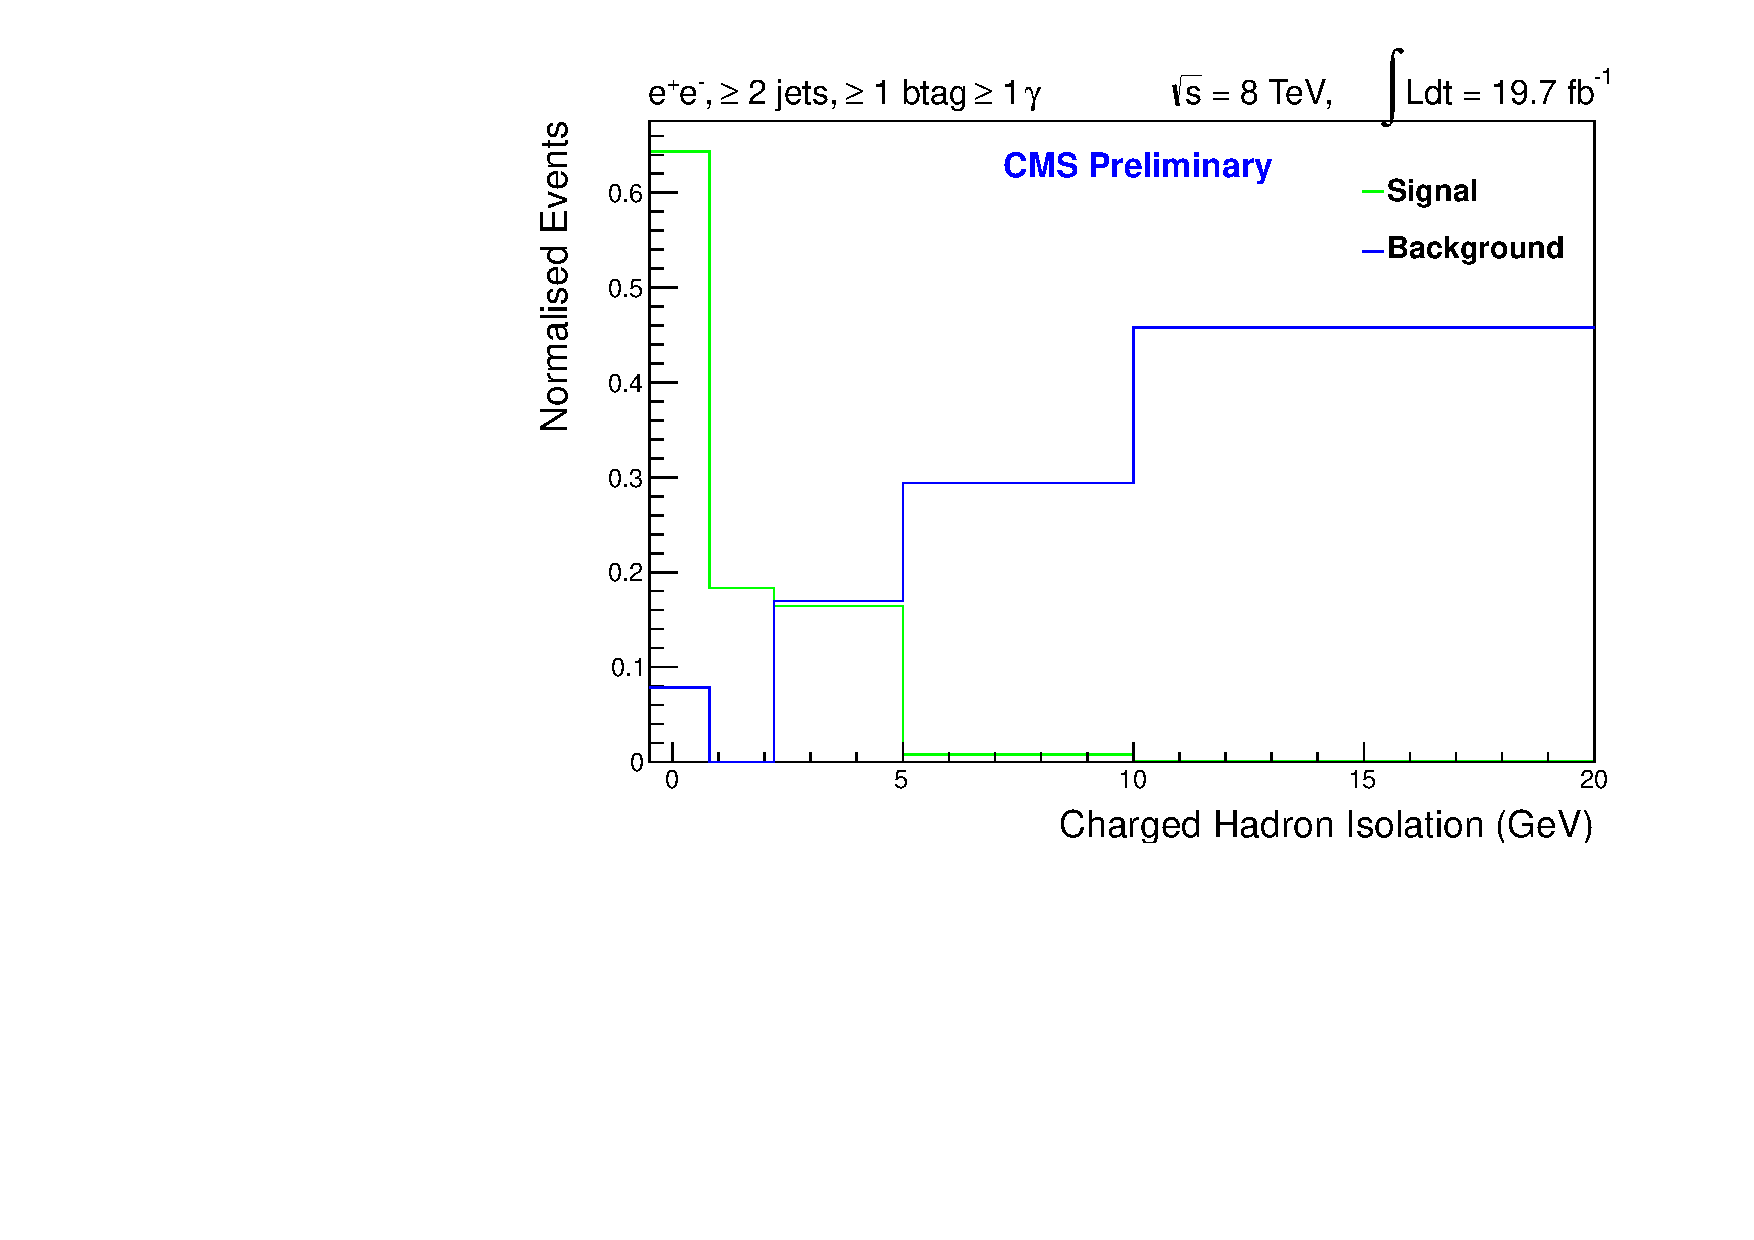
\includegraphics[width=0.5\textwidth]{Plots/Fits/TTbarPhotonAnalysis/EE/central/FitTemplate.pdf}\\
\begin{center}
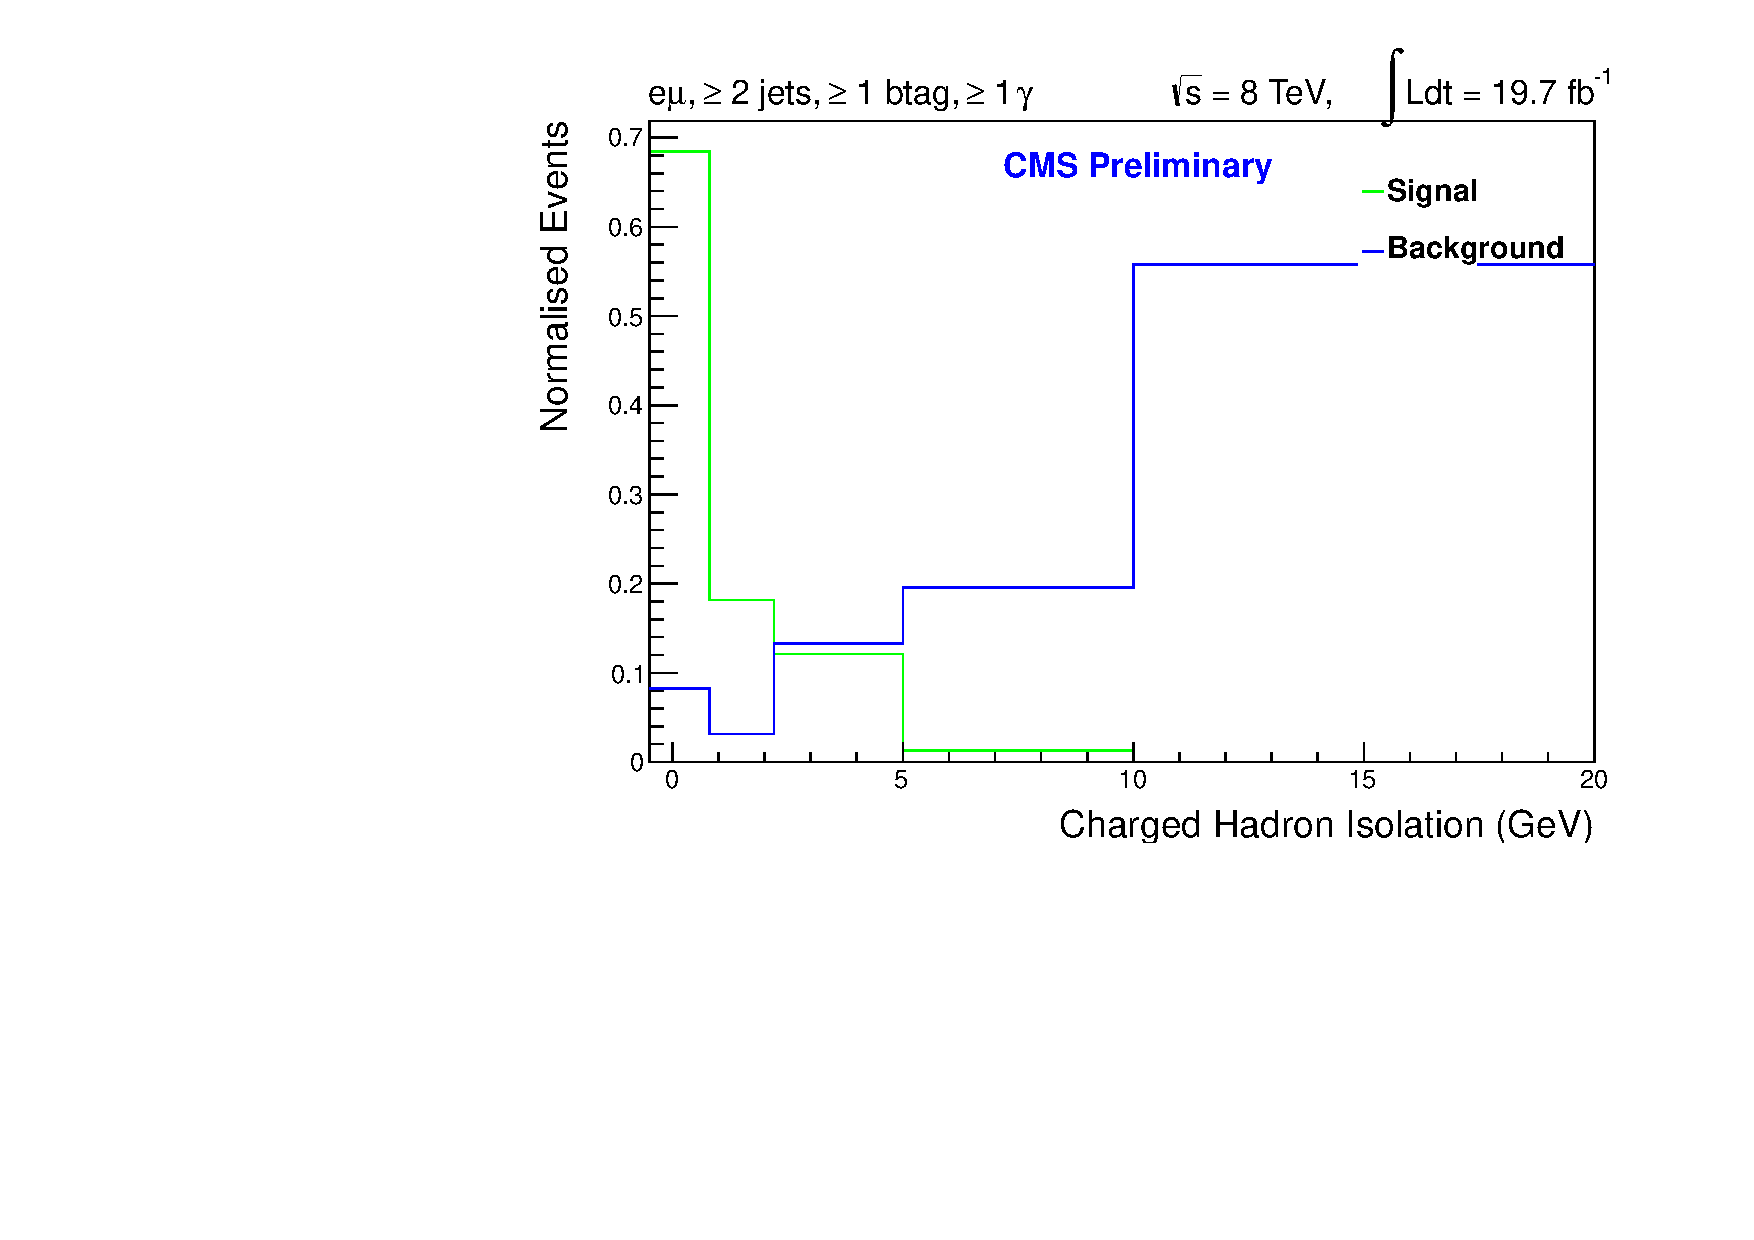
\includegraphics[width=0.5\textwidth]{Plots/Fits/TTbarPhotonAnalysis/EMu/central/FitTemplate.pdf}
\end{center}
\caption{Fit to charged hadron isolation templates in the $\mu^{+}\mu^{-}$, $e^{+}e^{-}$, and $e\mu$ channels.}
\label{fig-fitTemplates}
\end{figure}

\begin{figure}
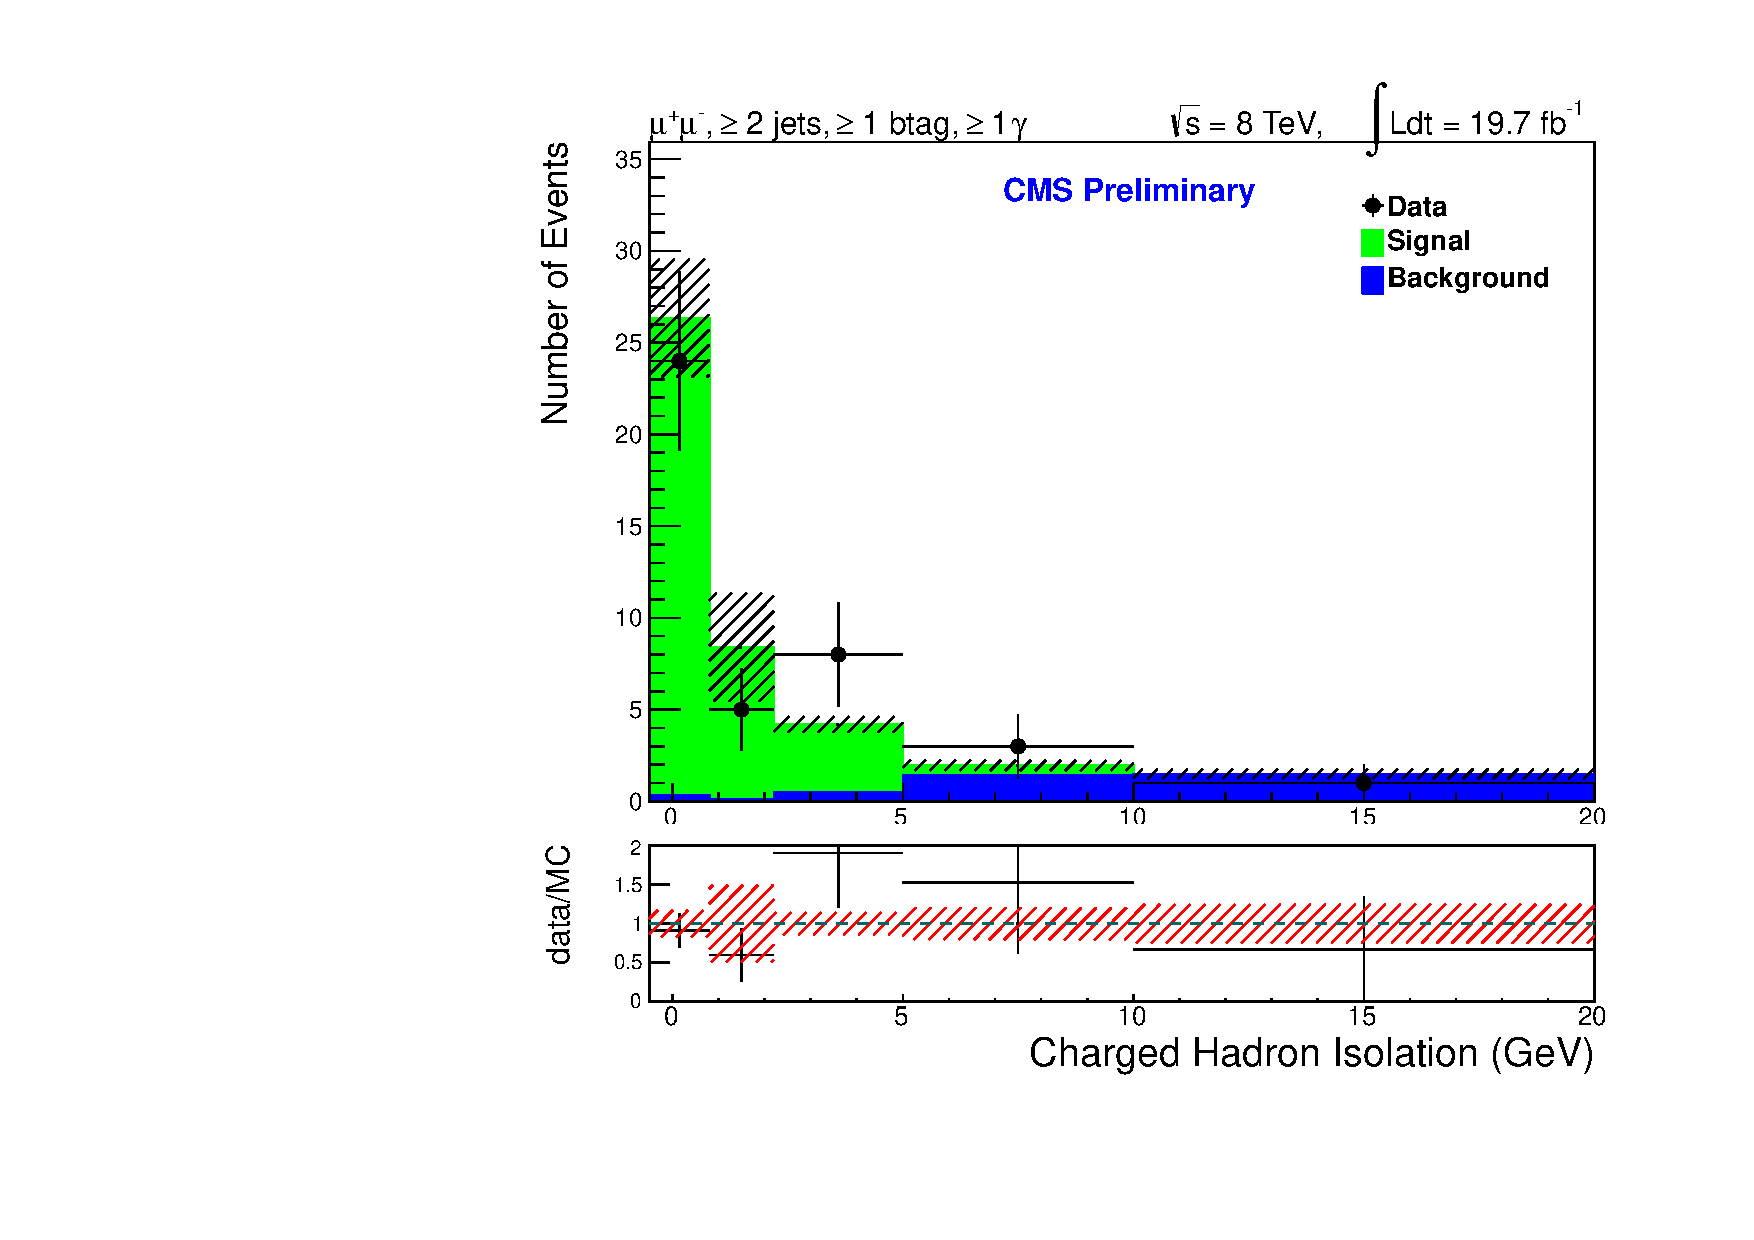
\includegraphics[width=0.5\textwidth]{Plots/Fits/TTbarPhotonAnalysis/MuMu/central/Fit.pdf}
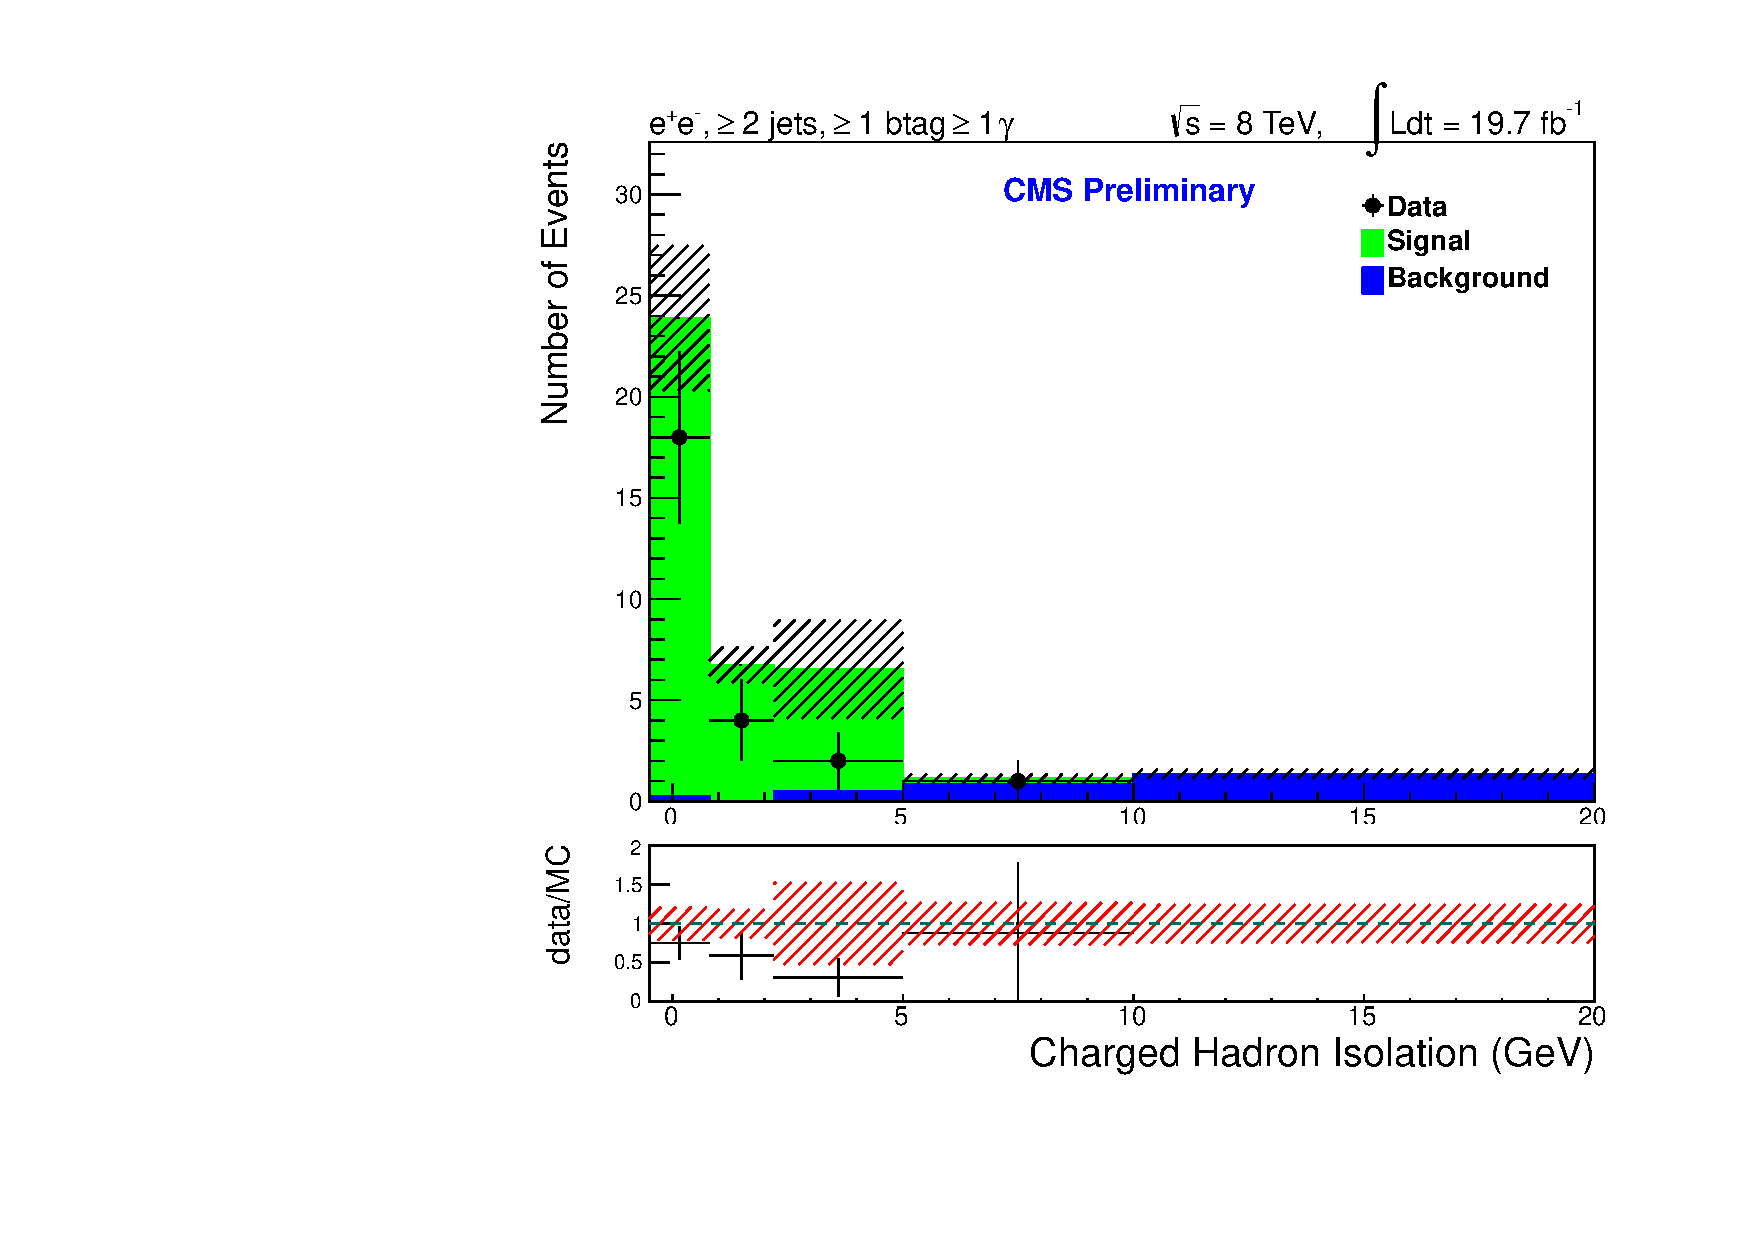
\includegraphics[width=0.5\textwidth]{Plots/Fits/TTbarPhotonAnalysis/EE/central/Fit.pdf}\\
\begin{center}
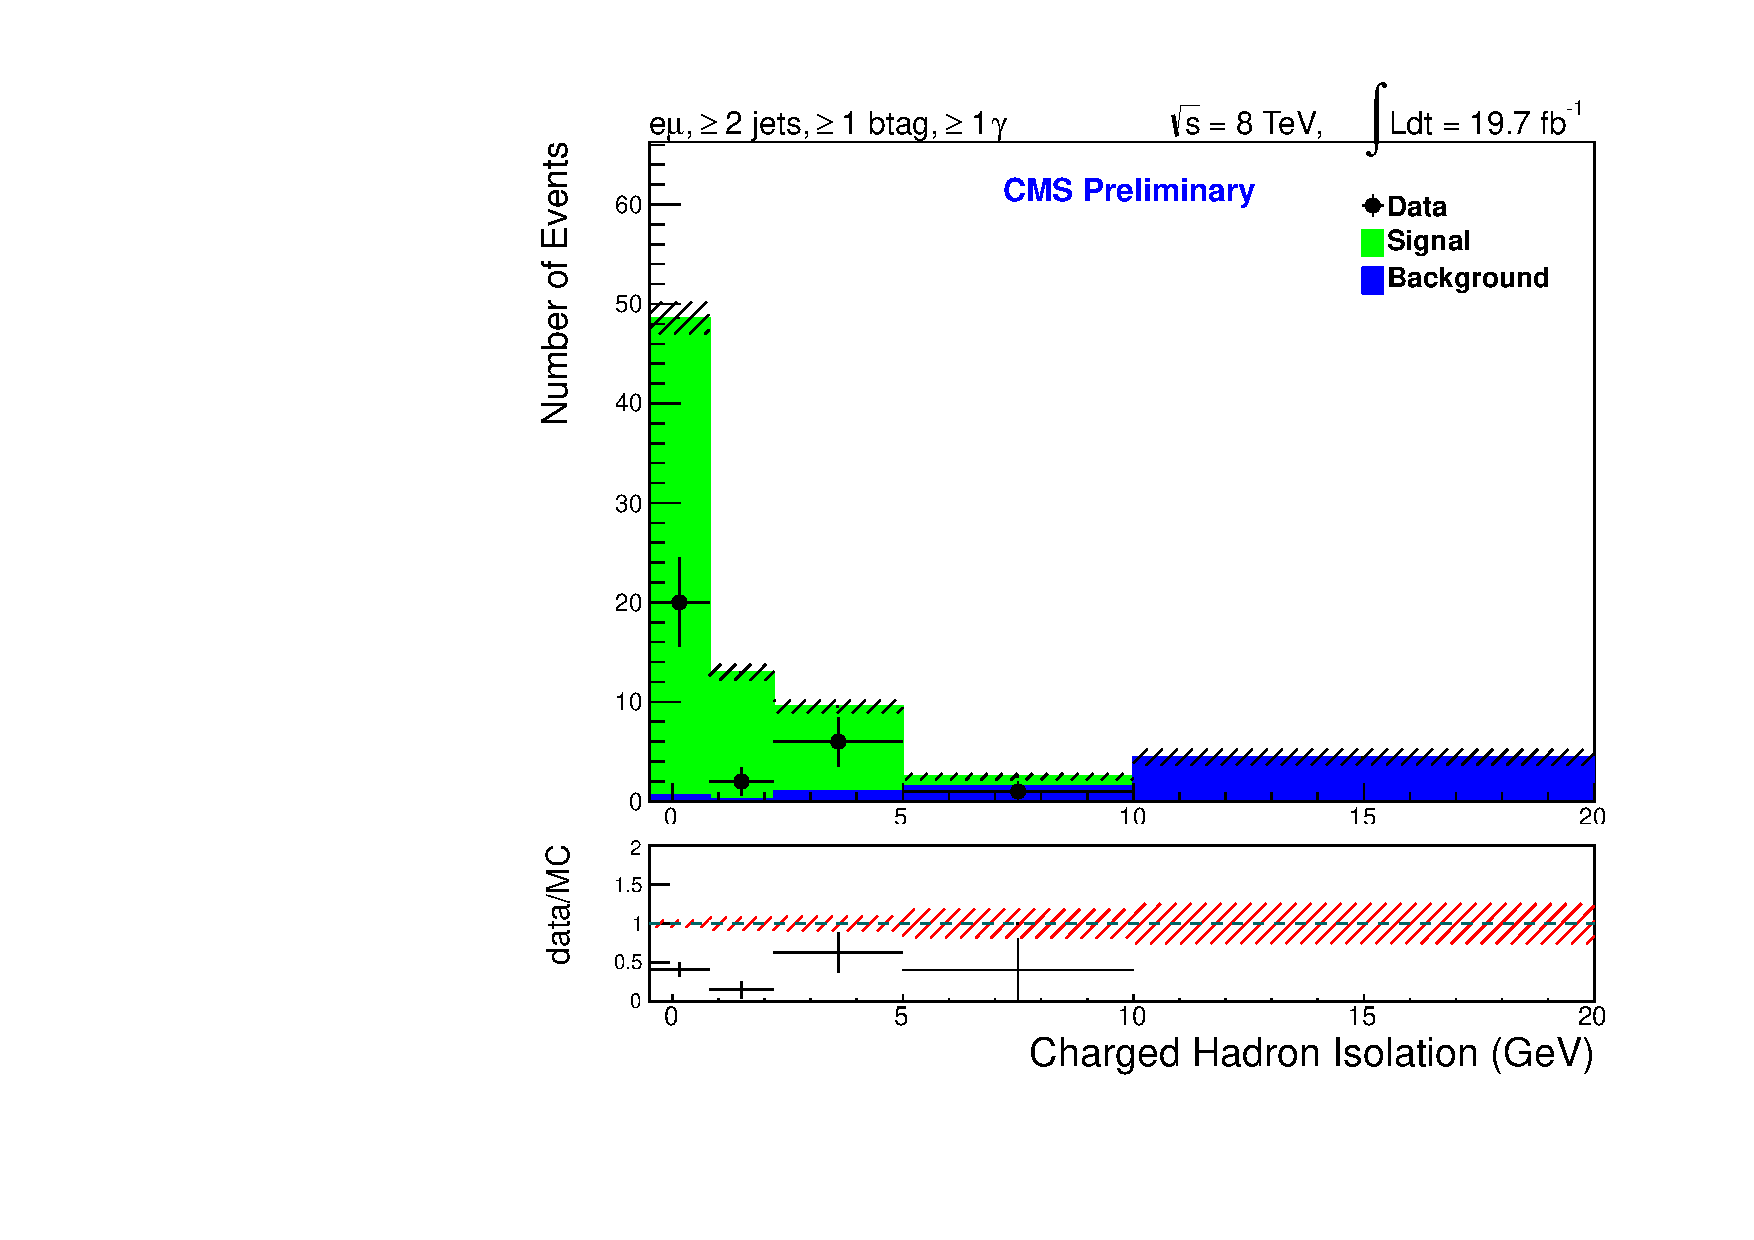
\includegraphics[width=0.5\textwidth]{Plots/Fits/TTbarPhotonAnalysis/EMu/central/Fit.pdf}
\end{center}
\caption{Fit to charged hadron isolation in the $\mu^{+}\mu^{-}$, $e^{+}e^{-}$, and $e\mu$ channels.}
\label{fig-fits}
\end{figure}



\begin{sidewaystable} 
\begin{center}
\begin{tabular}{|l|c|}
\hline
	\textbf{Dataset} & \textbf{Integrated Luminosity ($pb^{-1}$)}\\
\hline
	/DoubleMuParked/Run2012A-22Jan2013-v1/AOD  & 876 \\
	/DoubleMuParked/Run2012B-22Jan2013-v1/AOD  & 4412 \\
	/DoubleMuParked/Run2012C-22Jan2013-v1/AOD  & 7017 \\
	/DoubleMuParked/Run2012D-22Jan2013-v1/AOD  & 7369 \\
\hline
	Total & 19.7\\	
\hline
	/DoubleElectron/Run2012A-22Jan2013-v1/AOD  & 875 \\
	/DoubleElectron/Run2012B-22Jan2013-v1/AOD  & 4412 \\
	/DoubleElectron/Run2012C-22Jan2013-v1/AOD  & 7055 \\
	/DoubleElectron/Run2012D-22Jan2013-v1/AOD  & 7369 \\
\hline
	Total & 19.7\\	
\hline
	/MuEG/Run2012A-22Jan2013-v1/AOD  & 876 \\
	/MuEG/Run2012B-22Jan2013-v1/AOD  & 4411 \\
	/MuEG/Run2012C-22Jan2013-v1/AOD  & 7055 \\
	/MuEG/Run2012D-22Jan2013-v1/AOD  & 7360 \\
\hline
	Total & 19.7\\	
\hline	
\end{tabular}	
\end{center}
\caption{Dataset information for each run in each respective decay channel.}
\label{tab-datasets}
\end{sidewaystable}

